%\begin{abstract}
  We study the spatio-temporal behavior of the Els\"asser variables
  describing magnetic and velocity field fluctuations, using direct
  numerical simulations of three-dimensional magnetohydrodynamic
  turbulence. We consider cases with relatively small, intermediate,
  and large values of a mean background magnetic field, and with null,
  small, and high cross-helicity (correlations between the velocity
  and the magnetic field). Wavenumber-dependent time correlation
  functions are computed for the different simulations. From these
  correlation functions, the decorrelation time is computed and
  compared with different theoretical characteristic times: the local
  non-linear time, the random-sweeping time, and the Alfv\'enic
  time. It is found that decorrelation times are dominated by sweeping
  effects for low values of the mean magnetic field and for low values
  of the cross-helicity, while for large values of the background
  field or of the cross-helicity and for wave vectors sufficiently
  aligned with the guide field, decorrelation times are controlled by
  Alfv\'enic effects. Finally, we observe counter-propagation of
  Alfv\'enic fluctuations due to reflections produced by
  inhomogeneities in the total magnetic field. This effect becomes
  more prominent in flows with large cross-helicity, strongly
  modifying the propagation of waves in turbulent magnetohydrodynamic
  flows.
%\end{abstract}

%%%%%%%%%%%%%%%%%%%%%%%%%%%%%%%%%
\section{Introduction}\label{sec_Intro}

Las fluctuaciones turbulentas están presentes en un amplio rango de
escalas, tanto espaciales como temporales. En MHD incompresible, los
acoplamientos no lineales se basan en interacciones de tríadas de
modos \cite{zhou_non-gaussian_1993, alexakis_turbulent_2007,
  teaca_energy_2009, aluie_2010, mininni_scale_2011}, que pueden ser
de distintos tipos, tales como distorsiones no lineales de \eddies
(locales en el espacio de ondas) o de tipo barrido de escalas pequeñas
por escalas grandes (no locales en el espacio de Fourier)
\cite{kraichnan_structure_1959, tennekes_eulerian_1975,
  chen_sweeping_1989, nelkin_time_1990, matthaeus_eulerian_2010,
  servidio_time_2011, carbone_anisotropy_2011}.  Por supuesto, estos
acoplamientos no lineales también involucran interacciones con ondas
en el flujo, que son ubicuas tanto en los flujos MHD como en plasma
turbulento.

Las ecuaciones de MHD incompresible sustentan ondas de Alfvén, que en
la presencia de un campo magnético de fondo $\vec{B}_0'$ son
descriptas por una relación de dispersión lineal de frecuencia
$\omega=\vec{k} \cdot \vec{V}_\textrm{A}$ para el vector de onda
$\vec{k}$, con velocidad de Alfvén
$\vec{V}_\textrm{A}=\vec{B}_0'/\sqrt{4\pi \rho}$ y con densidad de
masa $\rho$.

Es sabido que estas ondas, cuando se consideran aisladamiente, son
también soluciones exactas de las ecuaciones no lineales de MHD ideal.
La presencia simultánea de fluctuaciones contrapropagantes, sin
embargo, activa las interacciones no lineales a lo largo de los modos,
produciendo dispersión, y en consecuencia las ondas dejan de ser
soluciones exactas del sistema
\cite{dobrowolny_1980_HydromagneticTurbulence}. Como el campo
magnético de fondo controla la velocidad de propagación (es decir, la
velocidad de Alfvén), la interacción no lineal está influenciada por
el {\color{red} Alfvén crossing time} de los paquetes de onda
contrapropagantes. Por lo tanto, existe una competencia entre las
interacciones no lineales (es decir, la turbulencia) y la propagación
de ondas \cite{dmitruk_waves_2009}.

La fuerza de las fluctuaciones contrapropagantes puede ser medida por
la helicidad cruzada, una cantidad que es un invariante cuadrático de
las ecuaciones de MHD ideal (ver Sec.~\ref{sec_EqNumSim}).  Esta
cantidad es, además, de relevancia para el viento solar y para los
plasmas espaciales, dado que los flujos de gran escala con helicidad
cruzada (en presencia de un campo guía) se encuentran usualmente en el
medio interplanetario. Entonces, se puede realizar un análisis
espacio-temporal del campo de fluctuaciones \cite{servidio_time_2011,
  clark_di_leoni_spatio-temporal_2015} para estudiar cuantitativamente
la importancia de estos diversos efectos, y poder así distinguir cual
es la escala de tiempo dominante entre las diversas posibilidades,
dependiendo de los distintos parámetros del sistema. Este tipo de
análisis ya fue realizado para flujos MHD sin helicidad cruzada
\cite{meyrand_weak_2015, lugones_2016_spatiotemporal,
  meyrand_direct_2016}, observando diferentes comportamientos
dependientes de si la turbulencia es débil o fuerte.  La conclusión
prevaleciente, para turbulencia fuerte, es que el tiempo de
descorrelación de los modos de Fourier en el rango inercial es
típicamente dominado por el \sweeping debido al flujo de gran escala
\cite{servidio_time_2011, chen_sweeping_1989,
  lugones_2016_spatiotemporal}.  No obstante, el efecto de cambiar la
fuerza de las fluctuaciones contrapropagantes en el comportamiento
espacio-temporal del flujo, y su tiempo de decorrelación, no fue
considerado previamente.

En el presente trabajo, realizamos un análisis espacio-temporal de la
turbulencia MHD, controlando simultánea y separadamente la intensidad
de campo magnético de fondo y la cantidad de helicidad cruzada en el
flujo, extendiendo así nuestro estudio previo
\cite{lugones_2016_spatiotemporal} de MHD incompresible con un campo
magnético de fondo y sin helicidad cruzada.  Presentamos varias
soluciones numéricas de las ecuaciones MHD incompresibles en un estado
turbulento estacionario, y analizamos cada escala temporal en el
sistema usando funciones de correlación dependientes del número de
onda y del tiempo, y espectros espacio-temporales de las variables de
Els\"asser.  El estudio espacio-temporal de las variables de
Els\"asser nos permite separar las dos posibles polarizaciones de las
ondas de Alfvén, así como también las direcciones de propagación, y
cuantizar cualquier desbalance entre las dos polarizaciones.
Encontramos que los tiempos de descorrelación son dominados por los
efectos de \sweeping para valores pequeños del campo magnético medio y
para valores bajos de la helicidad cruzada; mientras que para valores
grandes del campo de fondo o de la helicidad cruzada, los tiempos de
descorrelación son controlados por los tiempos de Alfvén.  Más aún,
para valores altos de la helicidad cruzada, también observamos
contrapropagación de las fluctuaciones de Alfvén (i.e., una inversión
en la dirección de propagación de una de las polarizaciones de las
ondas de Alfvén), causado por reflexiones en inhomogeneidades del
campo magnético total producidas por la turbulencia. Bajo ciertas
condiciones, esto puede resultar en la propagación de ambas
polarizaciones de las ondas de Alfvén en la misma dirección. Este
efecto afecta fuertemente las interacciones no lineales.

The structure of the paper is as follows. In Sec.~\ref{sec_EqNumSim}
we introduce the equations and the numerical methods employed, as well
as a description of the spatio-temporal spectrum and of the
correlation functions. Results are presented in
Sec.~\ref{sec_results}. Finally, discussions and conclusions are
presented in Sec.~\ref{sec_Conclusions}.

%%%%%%%%%%%%%%%%%%%%%%%%%%%%%%%%%%%%%%%%%
\section{Equations and numerical simulations}\label{sec_EqNumSim}

\subsection{The MHD equations and the Els\"asser fields}\label{sec_eq}
Las ecuaciones de MHD incompresible adimensionales (ecuaciones de
momento e inducción) son
\begin{equation}\label{eq:MHD_v}
  \frac {\partial \vec{v}}{\partial t} +
  \vec{v }\cdot \nabla \vec{v} = -\frac{1}{\rho}\nabla p +
  \vec{j} \times \vec{B} + \frac{1}{R} \nabla^2\vec{v} + \vec{F}_v,
\end{equation}
\begin{equation}\label{eq:MHD_b}
  \frac{\partial \vec{b}}{\partial t} = \nabla \times (\vec{v} 
  \times \vec{B}) + \frac{1}{R_m} \nabla^2 \vec{b} + \vec{F}_b,
\end{equation}
donde $\vec{v}$ es la velocidad del plasma,
$\vec{B} = \vec{b} + \vec{B}_0$ el campo magnético total (en unidades
de la velocidad de Alfvén, y obtenidas del campo magnético total
$\vec{B}'$ en unidades gaussianas luego de dividir por
$\sqrt{4\pi\rho}$, donde $\rho$ es la densidad del plasma), y
$\vec{F}_v$ y $\vec{F}_b$ son términos de forzado que luego serán
discutidos con más detalles.  El campo magnético total tiene una parte
fluctuante $\vec{b}$, y un campo medio DC
$\vec{B}_0=B_0\hat{x}$. Finalmente, $\vec{j} = \nabla \times \vec{b}$
es la densidad de corriente y $p$, la presión. Las unidades se basan
en la velocidad característica $v_0$, que para MHD es elegida como la
velocidad de Alfvén típica de las fluctuaciones del campo magnético,
$v_0 = \sqrt{\langle b^2 \rangle /(4\pi\rho)}$, donde
$\langle . \rangle$ denota promedio espacial. Los parámetros
adimensioanles que aparecen en la ecuación son los números de Reynolds
cinético y magnético, $R=v_0 L/\nu$ y $R_m = v_0 L /\mu$,
respectivamente, con $\nu$ la viscosidad cinemática, $\mu$ la
difusividad magnética, y $L$ la escala longitudinal característica (el
tamaño de la caja de la simulación está definido como $2\pi L$). La
unidad temporal es $t_0 = L/v_0$, que para MHD resulta ser el
{\color{red} Alfv\'en crossing time} basado en las fluctuaciones de
campo magnético. Los campos de Els\"asser vienen definidos como
\begin{equation}\label{eq:MHD_zdef}
\vec{z}^\pm = \vec{v} \pm \vec{b} .
\end{equation}

En términos de los campos de Els\"asser, las ecuaciones MHD pueden ser
escritas \cite{servidio_time_2011} como
\begin{equation}
\partial_t \vec{z}^\pm  = \pm  \vec{V}_\textrm{A} \cdot \nabla \vec{z}^\pm  - 
\vec{z}^\mp \cdot \nabla \vec{z}^\pm - \nabla{P} + 
\frac{1}{R} \nabla^2 \vec{z}^\pm ,
\label{eq:Elsasser}
\end{equation}
con $P=p/\rho$, y asumiendo que $R=R_m$. En el miembro derecho de la
\cref{eq:Elsasser}, escribimos explícitamente separado el término
convectivo en una parte lineal descripta por propagación Alfvénica con
$\vec{V}_\textrm{A} = \vec{B}_0$ la velocidad de Alfvén basada en el
campo magnético de fondo (con $\vec{B}_0$ el campo en unidades de
velocidad), y una parte no lineal describiendo la interacción entre
las fluctuaciones contrapropagantes tipo ondas. Es evidente a partir
de estas ecuaciones que ambos campos de Els\"asser deben estar
presentes para activar las interacciones no lineales.

Los invariantes ideales (i.e., con viscosidad y resistividad nula) de la teoría MHD incompresible pueden ser escritos en términos de los campos de Els\"asser.
La energía total $E$ (cinética más magnética) en términos de estas variables es
\begin{equation}
E = \frac{1}{2}\int{\left(\left|\vec{v}\right|^2 +
    \left|\vec{b}\right|^2 \right)\,dV} =
    \frac{1}{4}\int{\left(\left|\vec{z}^+\right|^2 +
    \left|\vec{z}^-\right|^2 \right)\,dV},
\label{eq:ener}
\end{equation}
mientras que la helicidad cruzada $H_c$ es
\begin{equation}
H_c = \int{\vec{v}\cdot\vec{b} \, dV} =
    \frac{1}{4}\int{\left(\left|\vec{z}^+\right|^2 
    - \left|\vec{z}^-\right|^2 \right)\,dV} .
\label{eq:cross}
\end{equation}
El cociente $\sigma_c = H_c/E$ mide la cantidad de fluctuaciones
contrapropagantes en el sistema. Un valor de $\sigma_c = \pm 1$
corresponde al caso con un único tipo de fluctuaciones $\vec{z}^\pm$,
mientras $\sigma_c=0$ representa equipartición entre ambos campos.

Siguiendo los trabajos de Matthaeus {\it et al.}
\cite{matthaeus1994transport} y Zhou {\it et al.}
\cite{zhou1990remarks}, las ecuaciones de MHD ideal pueden ser
linealizadas considerando la presencia de un campo magnéticoo
inhomogéneo de fondo y/o un flujo de fondo inhomogéneo, como
\begin{equation}\label{eq:MHD_zpzm}
  \partial_t \vec{z}^\pm
  + \left( L^\pm_\vec{x} + L^\pm \right) \vec{z}^\pm
  + M^\pm_{ik} \vec{z}^\mp_k
  = 0,
\end{equation}
Los operadores lineales $L^\pm_\vec{x}$, $L^\pm$, y $M^\pm_{ik}$
involucran gradientes actuando tanto el los campos a grandes escalas
como en pequeñas, y están dados por
\begin{equation}\label{eq:MHD_Lx}
  L^\pm_\vec{x} = \left( \vec{U} \mp \vec{V}_\textrm{A} \right) \cdot \nabla ,
\end{equation}
\begin{equation}\label{eq:MHD_L}
  L^\pm = \frac{1}{2} \nabla \cdot \left( \frac{\vec{U}}{2} \pm \vec{V}_\textrm{A} 
  \right) ,
\end{equation}
y
\begin{equation}\label{eq:MHD_Mik}
  M^\pm_{ik} = \nabla_k U_i \pm \frac{1}{\sqrt{4\pi\rho}} \nabla_k B_i'
  - \frac{1}{2} \delta_{ik} \nabla\cdot \left( \frac{\vec{U}}{2} \pm
  \vec{V}_\textrm{A} \right) ,
\end{equation}
donde $\vec{U}$ es el flujo de fondo. Aquí, tanto $\vec{U}$ como
$\vec{V}_\textrm{A}$ puede incluir inhomogeneidades de gran escala
(incluyendo, para $\vec{V}_\textrm{A}$, inhomogeneidades asociadas a
fluctuaciones de densidad).  Los términos de mezcla (aquéllos que
involucran los operadores $M_{ik}^\pm$) permiten la posibilidad de
crear fluctuaciones contrapropagantes a partir de una fluctuación
propagante de un único signo, por medio de reflexiones debidas a
inhomogeneidades en cualquiera de los campos de fondo
\cite{velli_1993_propagation}.  En este sentido, aun si el sistema
tiene condiciones iniciales con fluctuaciones propagantes de un único
signo, las reflexiones por las inhomogeneidades de los campos de fondo
crearán una cantidad de fluctuaciones contrapropagantes que generarán
interacciones no lineales, produciendo dispersión y turbulencia
\cite{matthaeus_1999_coronal, dmitruk_2001_coronal}. Pero este efecto
también puede resultar, en flujos con ambas polarizaciones de
excitaciones Alfvénicas, en contrapropagaciones de una de las
excitaciones, como mostraremos a partir de datos numéricos en la
sección \ref{sec_results}.

\subsection{Wavenumber-frequency spectrum and correlation functions}\label{sec_Wfspectrum_and_Gamma}

Usando argumentos de escala, es posible estimar diferentes tiempos
característicos en el sistema. El tiempo del \textit{eddy turnover}
local (o la escala temporal isotrópica no lineal) puede definirse como
$\tau_{nl} \sim 1/\left[ k v(k) \right]$, donde $v(k)$ es la amplitud
de las fluctuaciones de velocidad en la escala $\sim
1/k$. Considerando un escaleo de tipo Kolmogorov,
$v(k) \sim v_{rms} \left(kL\right)^{-1/3}$, el tiempo no lineal puede
ser escrito, en el rango inercial, como
\begin{equation}
\tau_{nl} = C_{nl} \left [
   v_{rms} L^{-1/3} \left(\sqrt{k^2_\perp +
   k^2_\parallel}\right)^{2/3}\right ]^{-1},
\label{eq:taunl}
\end{equation}
donde $C_{nl}$ es una constante adimensional de orden $1$, y
$k_\parallel$ y $k_\perp$ denotan los números de onda paralelo y
perpendicular al campo magnético de fondo. Aquí,
$v_{rms} = \left\langle |\vec{v}|^2 \right\rangle ^{1/2}$ es una
cantidad global, dominada por las contribuciones de las grandes
escalas \cite{zhou_magnetohydrodynamic_2004,
  matthaeus_anisotropic_2009}.

{\color{red}Another time decorrelation effect is governed by the
  sweeping characteristic time}, que a escala $\sim 1/k$ puede ser
expresado como
\begin{equation}
\tau_{sw} = C_{sw} \left( v_{rms}\sqrt{k^2_\perp + k^2_\parallel}
    \right)^{-1} .
\label{eq:tausw}
\end{equation}
Este tiempo corresponde a la advección de estructuras de pequeña
escala por el flujo de gran escala. Finalmente, el tiempo de Alfvén
característico puede ser definido como
\begin{equation}
\tau_A= C_A \left( v_A k_\parallel \right)^{-1} .
\label{eq:taua}
\end{equation}
En las últimas dos expresiones, $C_{sw}$ y $C_A$ son también
constantes adimensionales de orden $1$.

Estas no son todas las escalas temporales que podrían estar presentes
en turbulencia MHD, pero son las más relevantes para las discusiones
en las próximas secciones.  Como ejemplo, otra escala temporal que
amerita mención es el tiempo de doscorrelación de los momentos triples
cuando no hay equipartición entre las energías cinética y magnética,
por ejemplo en el contexto de dínamo \cite{baerenzung_2008_spectral}.

Para separar estas escalas temporales en el flujo, y para identificar
cuál es la escala temporal más relevante a una dada escala espacial,
se pueden utilizar dos herramientas: las propiedades estadísticas de
la función de correlación en tiempo y espacio, y el espectro en
números de onda y frecuencias. Empezaremos introduciendo este
último. Las estadísticas de los campos de Els\"asser pueden ser
caracterizadas por la función de autocorrelación espacio-temporal a
dos puntos \cite{servidio_time_2011},
\begin{equation}
  R^\pm(\vec{r},\tau) = \left\langle \vec{z}^\pm( \vec{x},t) \cdot
    \vec{z} ^\pm( \vec{x} + \vec{r},t+\tau) \right\rangle \Big/ 
  \left\langle \left|{\vec{z}^\pm}\right|^2 \right\rangle.
  \label{eq:Rzij}
\end{equation}
La transformada de Fourier en $\vec{r}$ desemboca en una densidad
espectral retrasada en eltiempo, que puede ser a su vez factorizada
como $S(\vec{k},\tau) = S(\vec{k})\Gamma(\vec{k},\tau)$. La función
$\Gamma(\vec{k},\tau)$ es la función de correlación dependiente de la
escala \cite{heisenberg_zur_1948,
  comte-bellot_simple_1971,orszag_numerical_1972}, la cual describe el
tiempo de descorrelación de cada modo espacial $\vec{k}$, es decir, la
memoria de las fluctuaciones con logitudes características de orden
$k_x^{-1}$, $k_y^{-1}$, y $k_z^{-1}$.

\begin{figure}
\centering
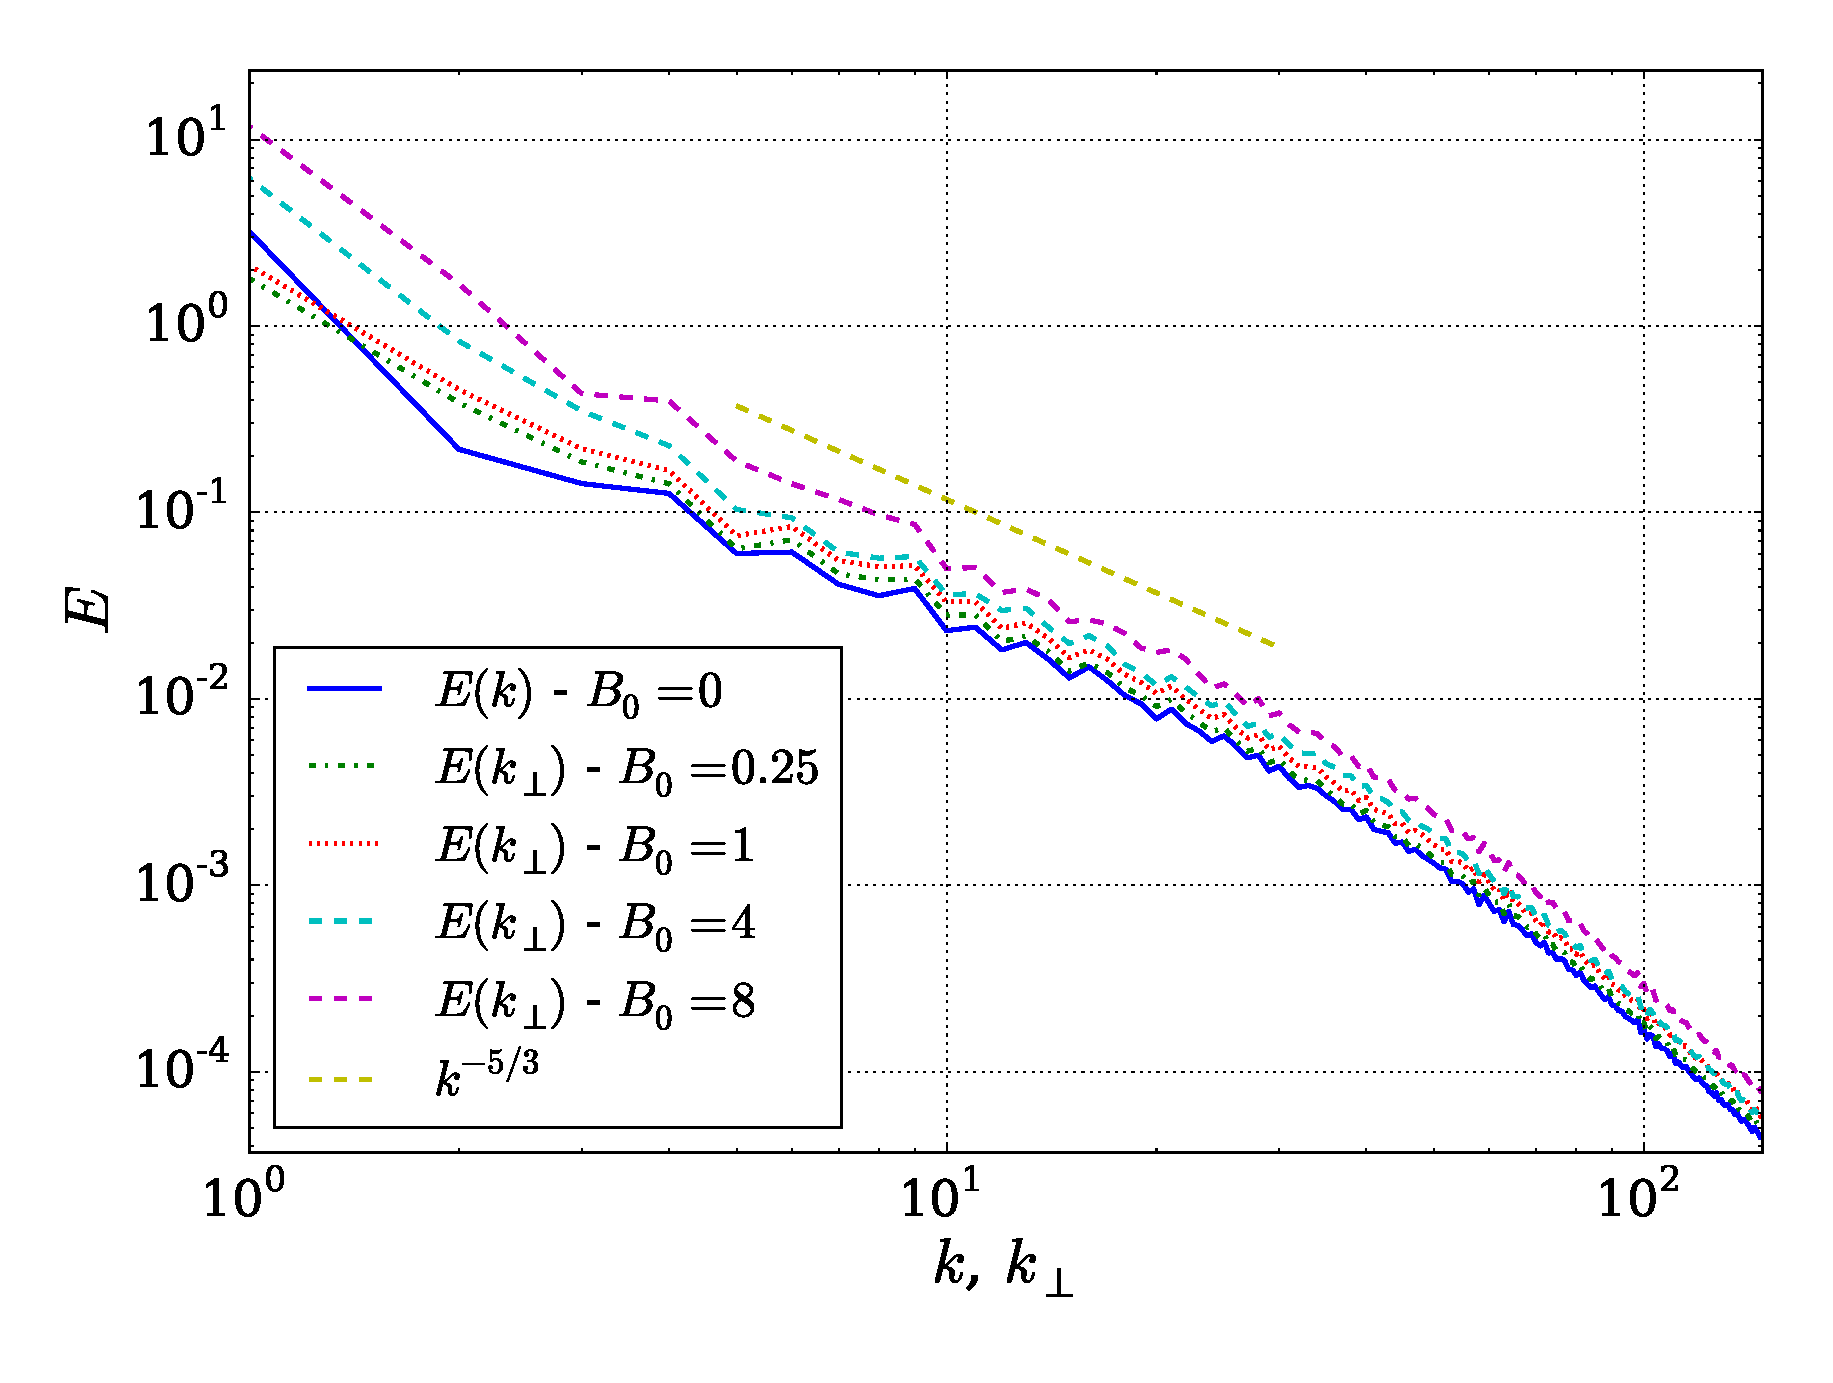
\includegraphics[width=1\columnwidth]{CrossHelicity/fig1_E.eps}
\caption{Reduced perpendicular energy spectra $E(k_\perp)$ for
  simulations with $B_0=0$, $0.25$, $1$, $2$, $4$, and $8$. All curves
  correspond to the case $\sigma_c = 0.3$, but the cases with $\sigma_c = 0$ and
  $0.9$ show the same behavior. Kolmogorov scaling,
  $\sim k_\perp^{-5/3}$, is shown as reference.}
\label{fig1:E}
\end{figure}

Cuando hay una dirección preferencial en el flujo (como en el presente
caso de turbulencia MHD con un campo magnético guía), es util asumir
simetría axial en el espacio de Fourier y escribir
$\Gamma(\vec{k},\tau) = \Gamma(k_\perp,k_\parallel,\tau)$. Como esta
función es tridimensional, también es útil estudiar
$\Gamma(k_\perp,k_\parallel,\tau)$ con uno de los argumentos fijos;
por ejemplo, fijando el valor de $k_\perp$ y analizando
$\Gamma(k_\perp,k_\parallel,\tau)$ en función de $k_\parallel$ y
$\tau$, obtenemos información de las fluctuaciones que varían sólo en
la dirección paralela, lo que nos permite distinguir entre
descorrelaciones que surgen de las interacciones no lineales de Alfvén
o del \sweeping.

La transformada de Fourier respecto del tiempo de la función de
correlación dependiente de la escala, da como resultado el espectro en
números de onda y frecuencias $E^\pm(\vec{k},\omega)$
\cite{clark_di_leoni_quantification_2014,
  clark_di_leoni_spatio-temporal_2015}, para cada uno de los campos de
Els\"asser. Estos espectros permiten la identificación de modos que
satisfacen una relación de dispersión generalizada del sistema, y
proveen una medida directa de cuánta energía hay en dichos modos, y de
cuánta energía hay en otros modos. Para los dos campos de Els\"asser,
a partir de las \cref{eq:ener, eq:cross} es fácil de ver que
\begin{equation}
  E = E^+ + E^- , \,\,\,\, H_c = E^+ - E^- ,
\end{equation}
donde $E^\pm = \int |\vec{z}^\pm|^2/4 \, dV$. Entonces, para el
espectro en números de onda y frecuencias de los campos de Els\"asser,
valen las siguientes dos relaciones
\begin{eqnarray}
  E^+(\vec{k},\omega) &=& [E(\vec{k},\omega) + H_c(\vec{k},\omega)]/2, \\
  E^-(\vec{k},\omega) &=& [E(\vec{k},\omega) - H_c(\vec{k},\omega)]/2.
\end{eqnarray}
En consecuencia, computar los espectros en números de onda y
frecuencias de la energía y de la helicidad cruzada, permite ls
determinación unívoca de los espectros para los campos de Els\"asser
fields, y viceversa.

\begin{figure*}
  \centering
  \subfigure[$B_0=0$]{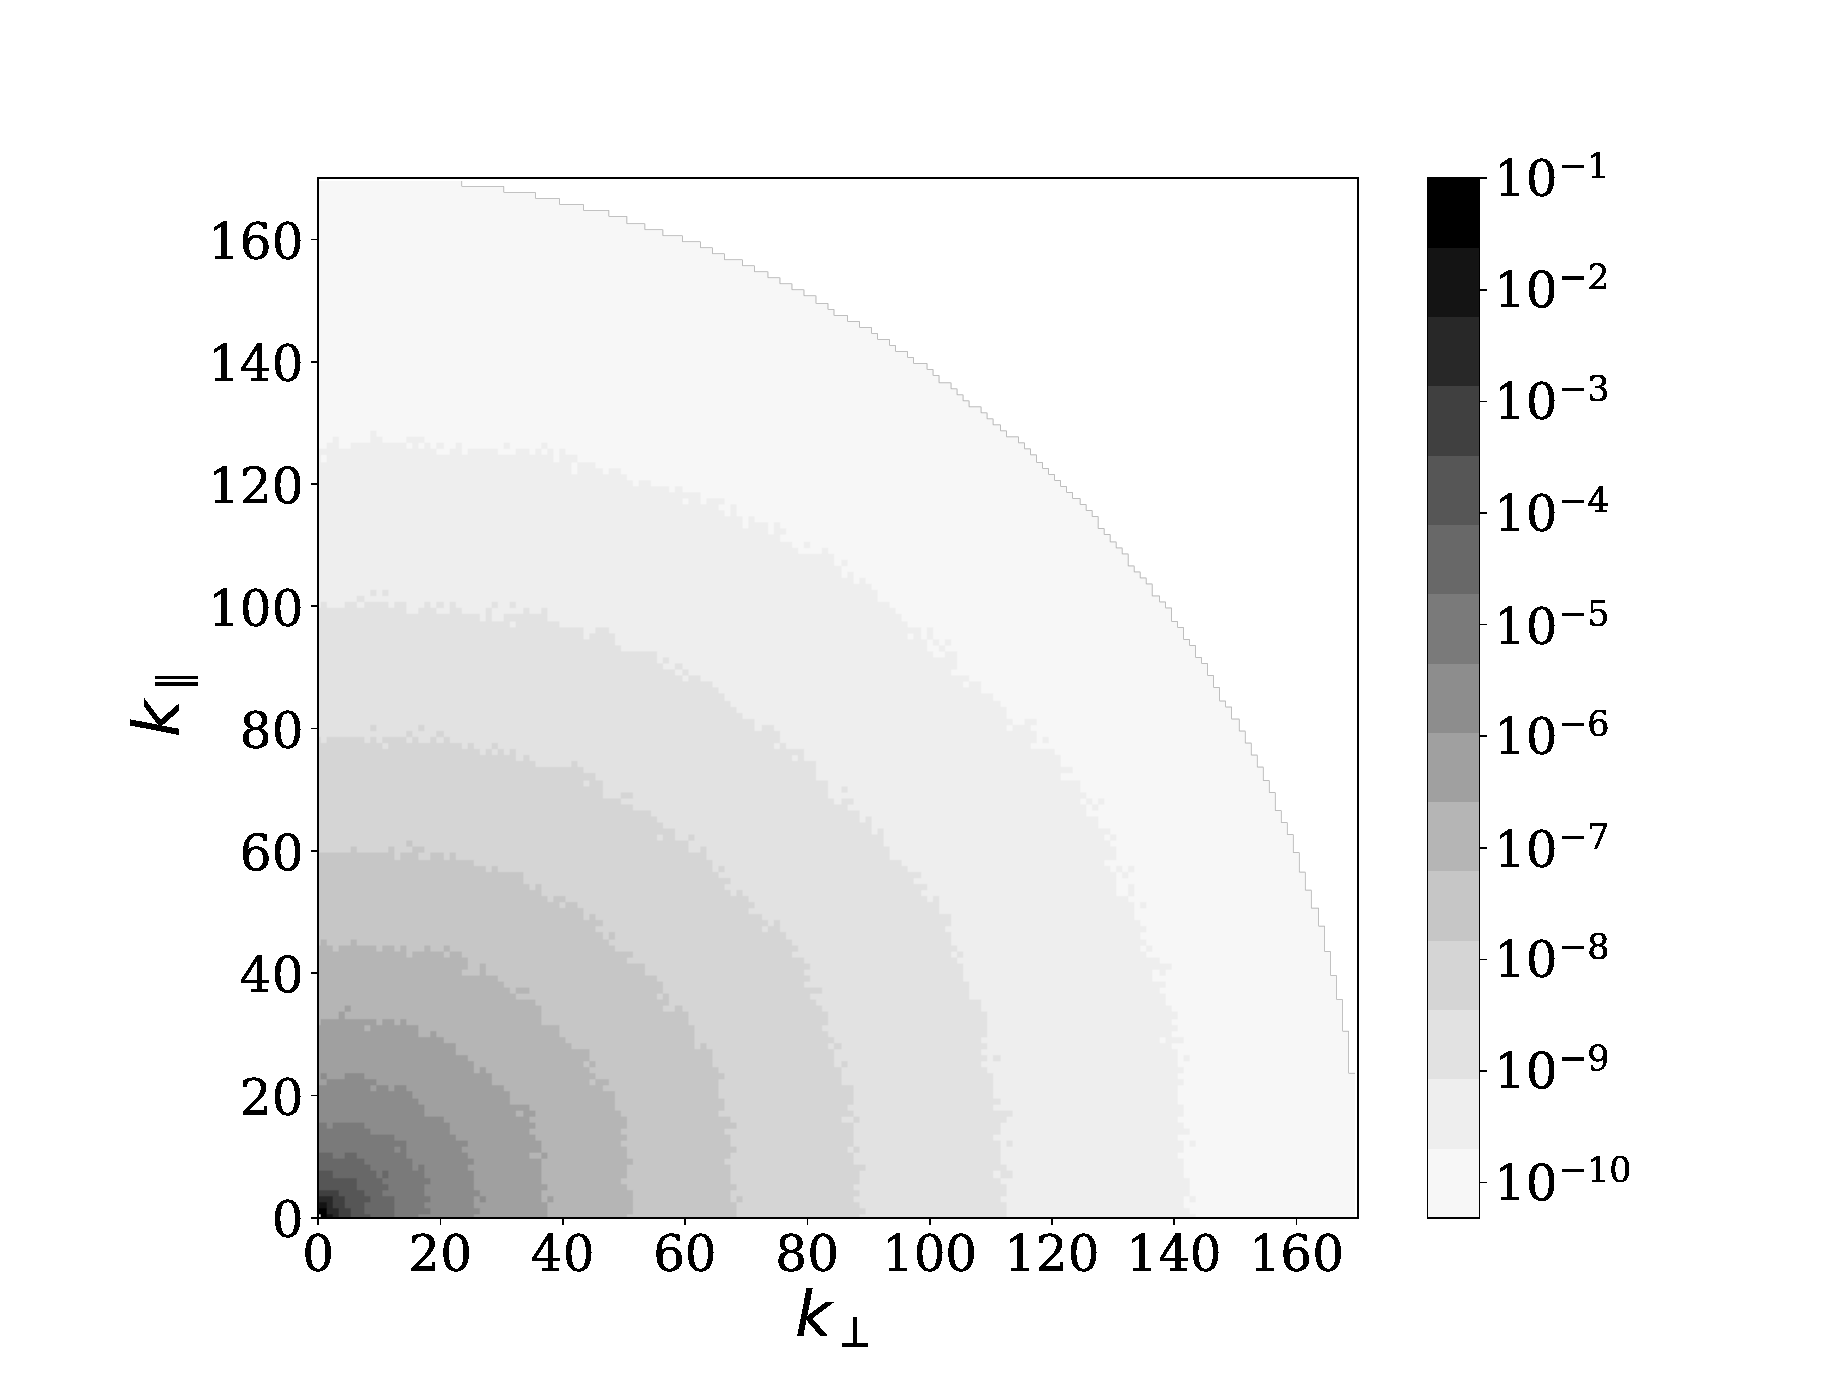
\includegraphics[width=0.48\textwidth]{CrossHelicity/fig2_B0_Hc03.eps}}
  \subfigure[$B_0=1$]{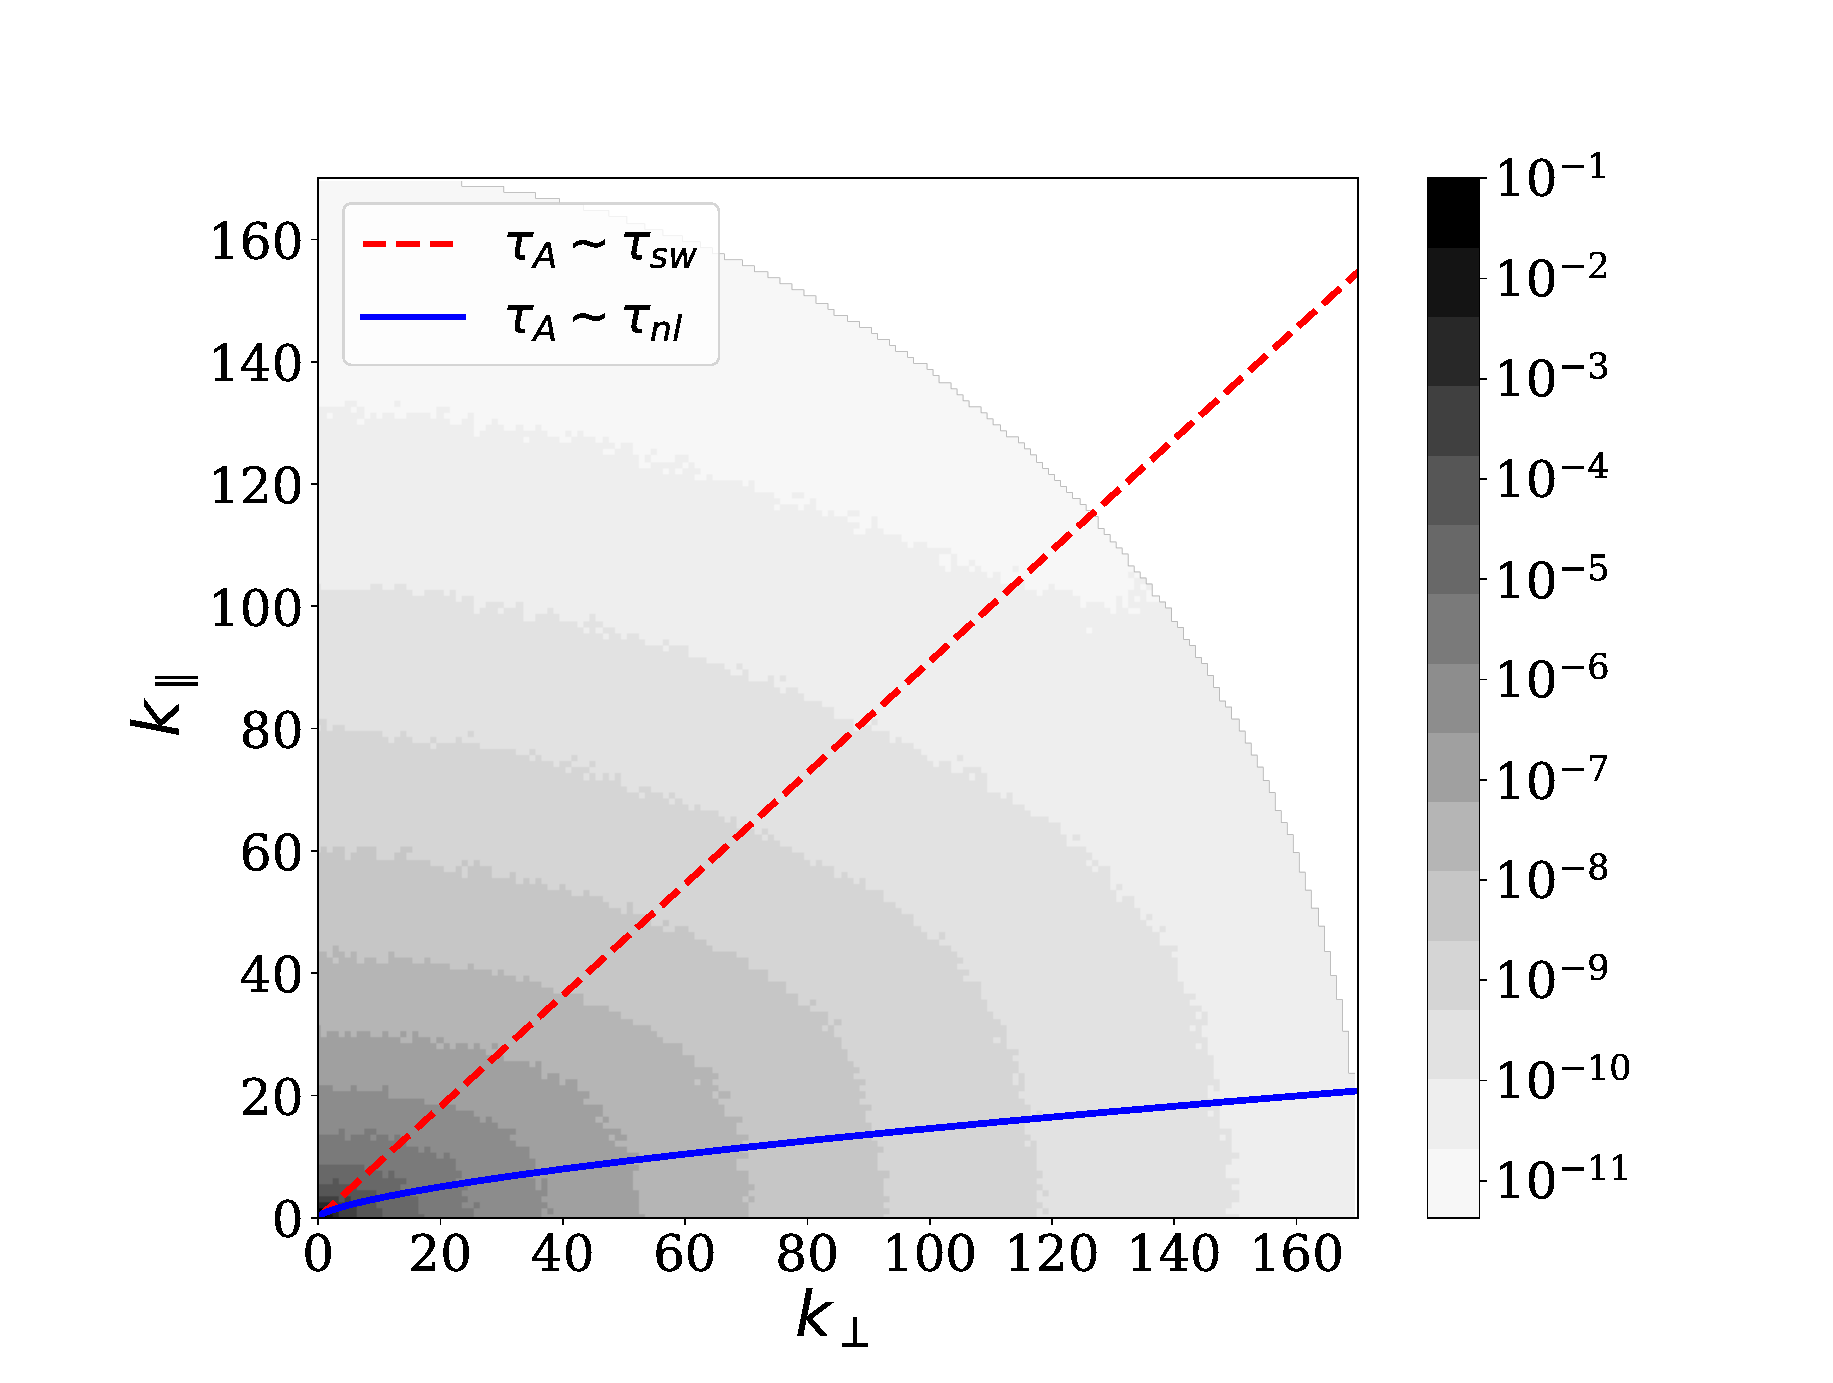
\includegraphics[width=0.48\textwidth]{CrossHelicity/fig2_B1_Hc03.eps}}
  \subfigure[$B_0=4$]{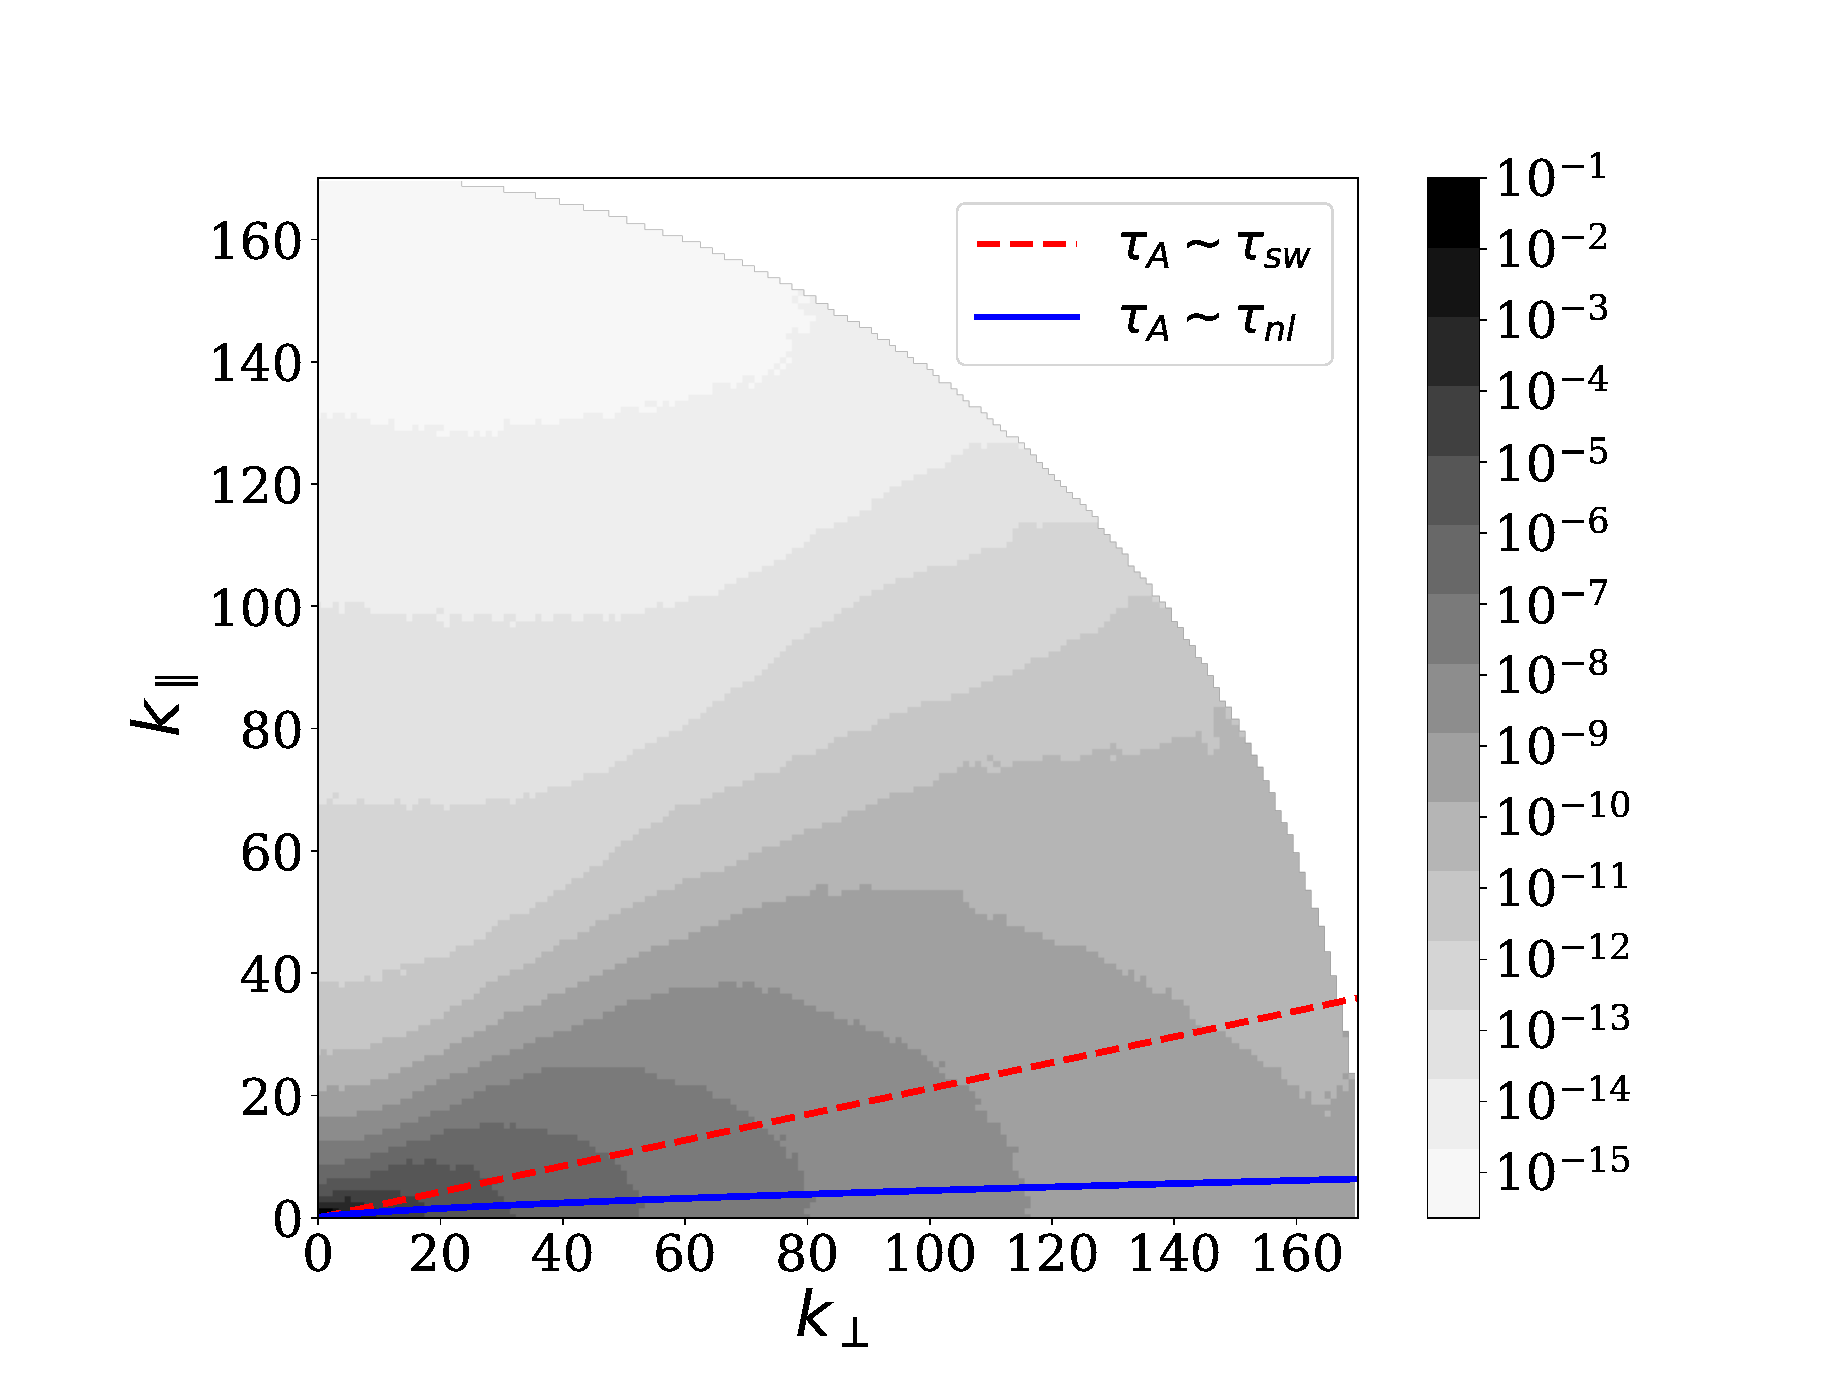
\includegraphics[width=0.48\textwidth]{CrossHelicity/fig2_B4_Hc03.eps}}
  \subfigure[$B_0=8$]{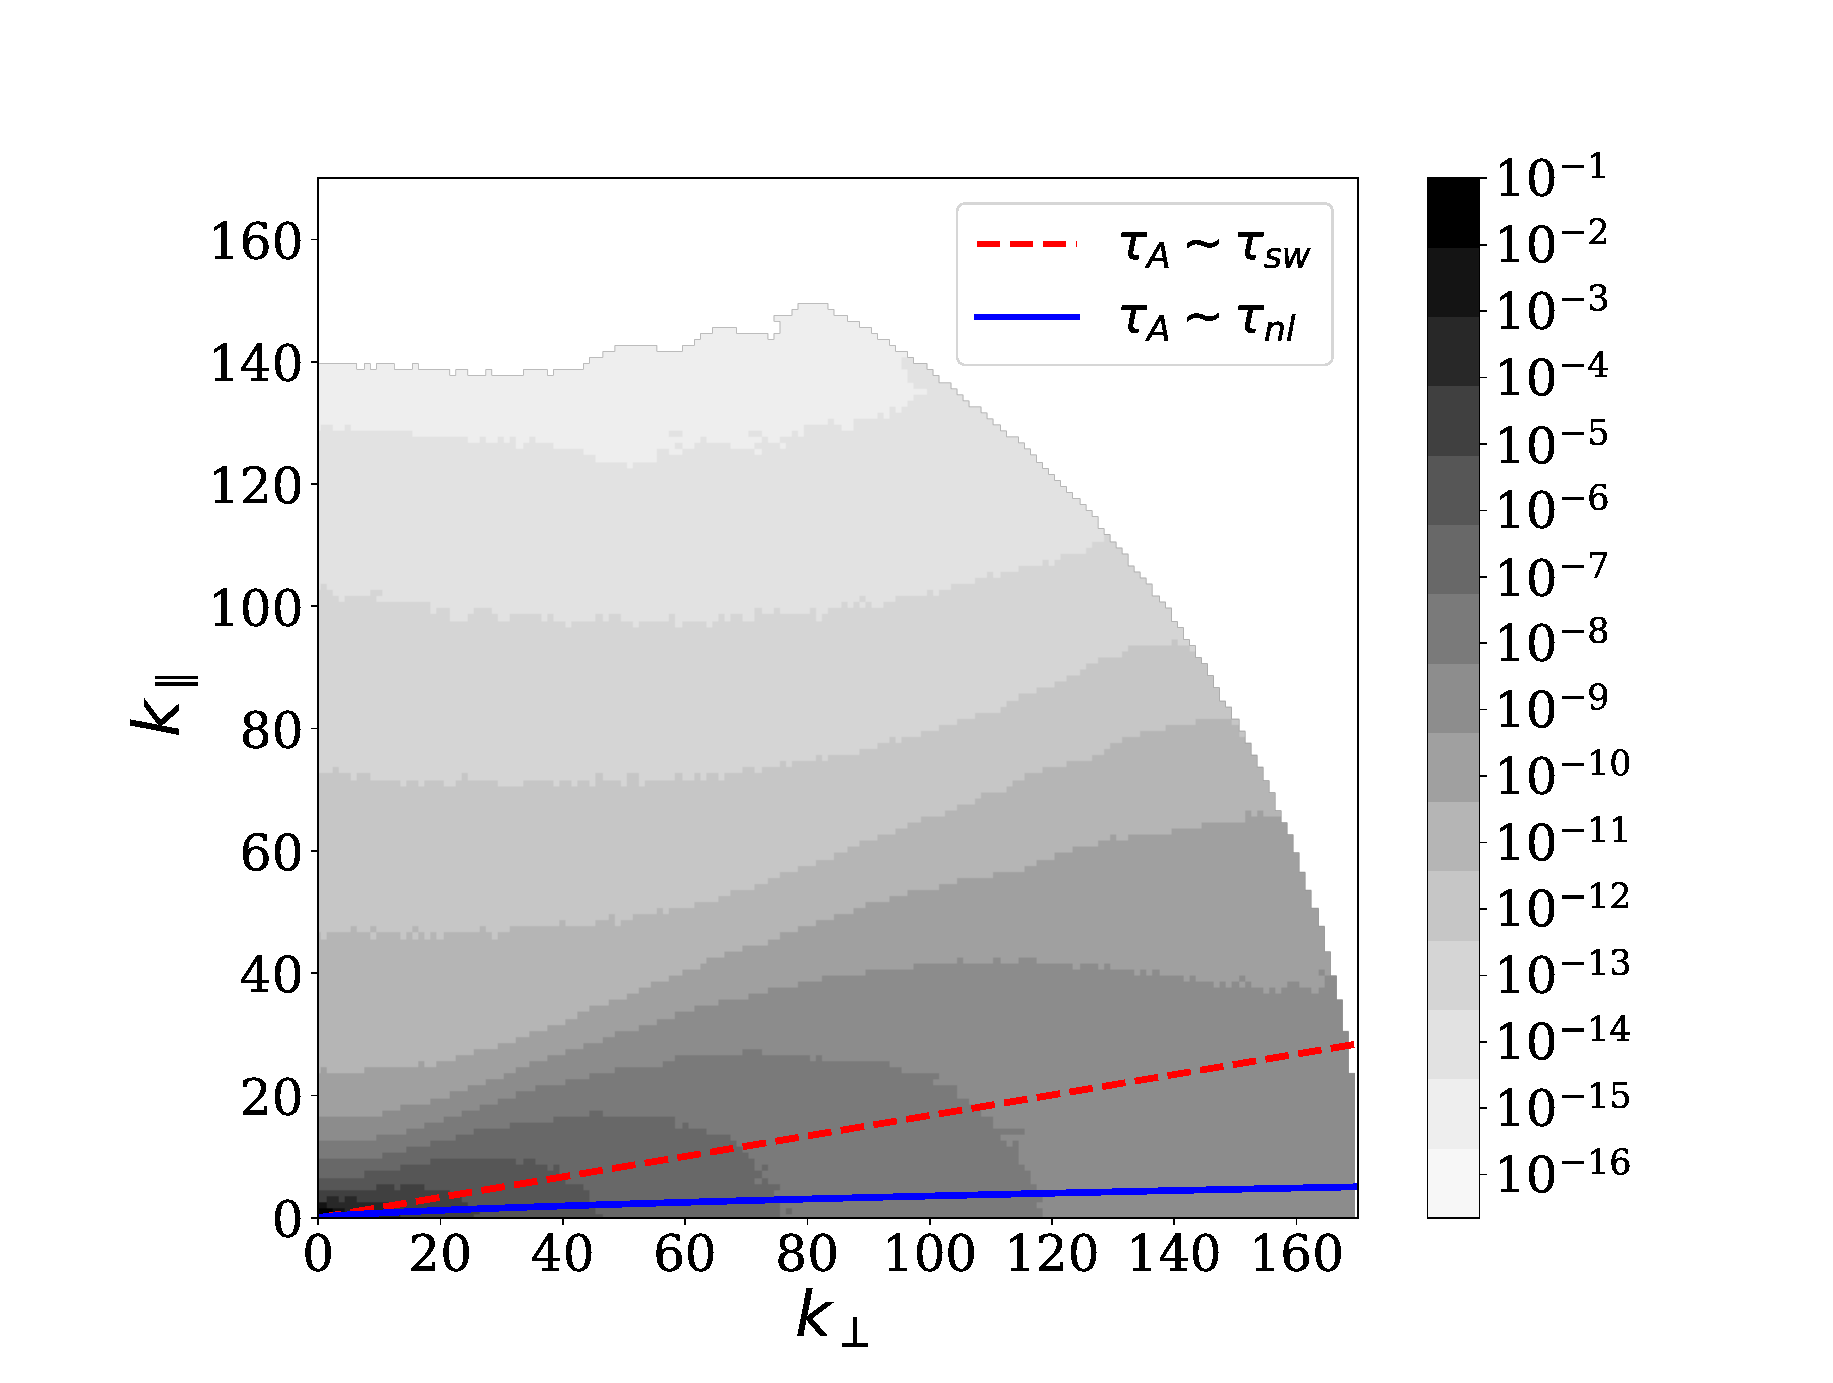
\includegraphics[width=0.48\textwidth]{CrossHelicity/fig2_B8_Hc03.eps}}
  \caption{Isocontours of the axisymmetric energy spectrum
    $e(k_\perp,k_\parallel)$ for $B_0=0$, $1$, $4$ and $8$, and for
    $\sigma_c = 0.3$. In all cases, dark means larger energy density (in
    logarithmic scale). The lines indicate the modes for which the
    sweeping time (red dashed line) or the local non-linear time
    (solid blue line) become equal to the Alfv\'en time. For large
    $B_0$ the flow becomes more anisotropic, and isocontours change
    shape as they cross these lines. Note also the increase in the
    energy in modes that have the Alfv\'en time as the fastest time
    (i.e., of modes below the solid blue curve) as $B_0$ increases.}
  \label{fig2:isocontourns}
\end{figure*}

\subsection{Numerical simulations}\label{sec_NumSim}

Para resolver numéricamente las ecuaciones de MHD incompresible,
empleamos un código pseudoespectral estándar
\cite{gomez_parallel_2005, gomez_mhd_2005, hybrid2011}. Consideramos
una resolución espacial de $N^3 = 512^3$ puntos de grilla, con un
esquema de integración temporal de Runge-Kutta de segundo orden.  La
resolución espacial es moderada, dado que necesitamos guardar una gran
cantidad de datos en el espacio y el tiempo para poder calcular las
funciones de correlación y los espectros definidos en la sección
\ref{sec_Wfspectrum_and_Gamma}. Los valores considerador para la
intensidad del campo magnético externo son $B_0 = 0, 0.25$, $1$, $2$,
$4$ y $8$ (en unidades del valor inicial r.m.s. de las fluctuaciones
magnéticas). Asumimos condiciones periódicas de contorno en un cubo de
lado $2\pi L$ (con $L$ la longitud de correlación inicial de las
fluctuaciones, definida como la unidad de longitud. Se removió el
\textit{aliasing} utilizando el método de truncamiento de la regla de
los dos-tercios.

\begin{figure*}
  \centering 
  \subfigure[$B_0 = 0$, $\vec{z}^-$, $\sigma_c = 0.3$]{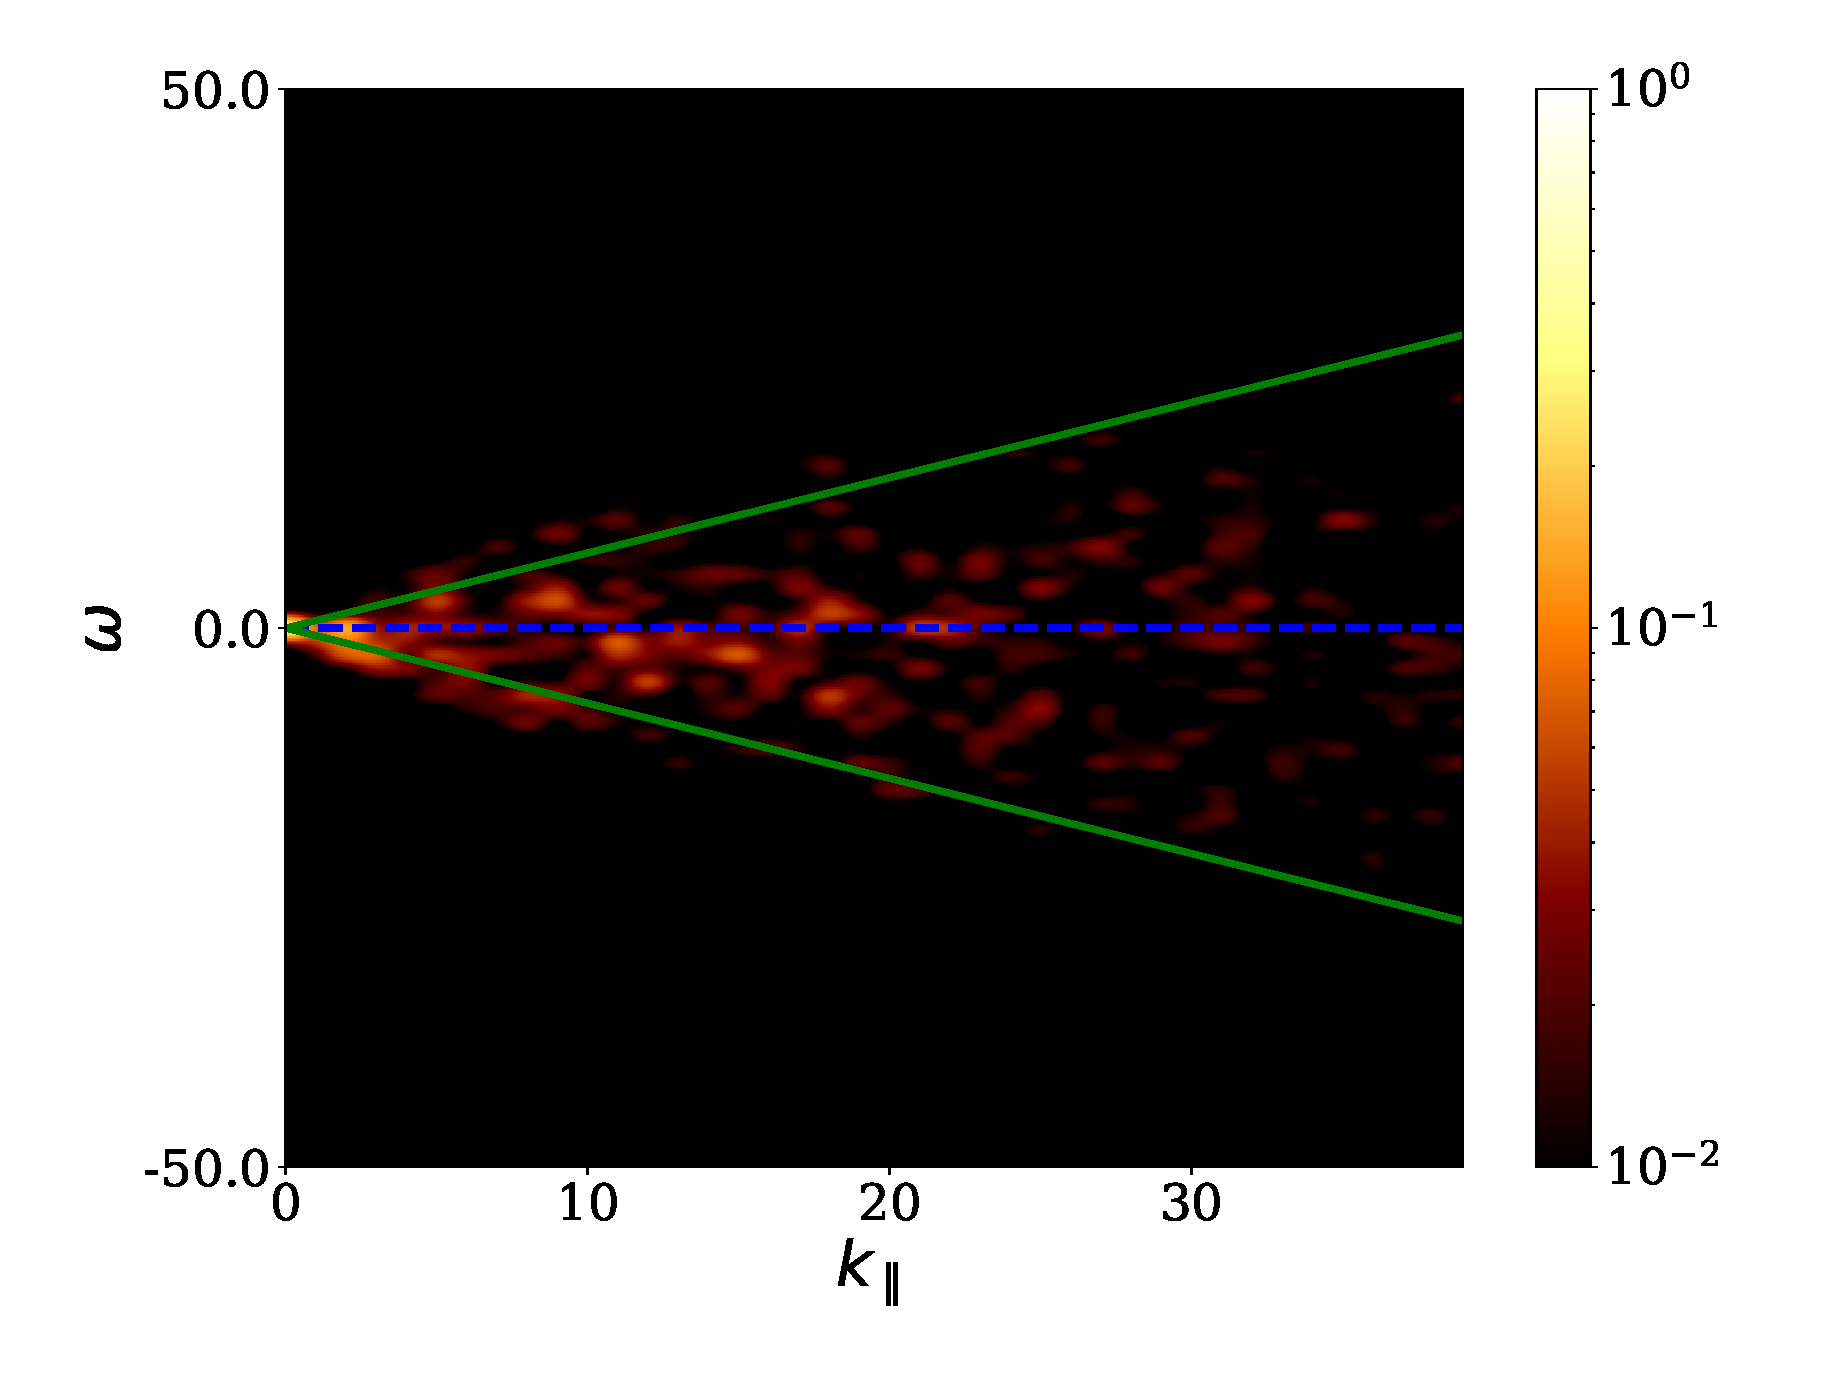
\includegraphics[width=0.45\textwidth]{{CrossHelicity/fig3_B0.0_y_Hc0.3_zm_kperp0}.eps}}
  \subfigure[$B_0 = 0$, $\vec{z}^+$, $\sigma_c = 0.3$]{\includegraphics[width=0.45\textwidth]{{CrossHelicity/fig3_B0.0_y_Hc0.3_zp_kperp0}.eps}}
  \subfigure[$B_0 = 0$, $\vec{z}^-$, $\sigma_c = 0.9$]{\includegraphics[width=0.45\textwidth]{{CrossHelicity/fig3_B0.0_y_Hc0.9_zm_kperp0}.eps}}
  \subfigure[$B_0 = 0$, $\vec{z}^+$, $\sigma_c = 0.9$]{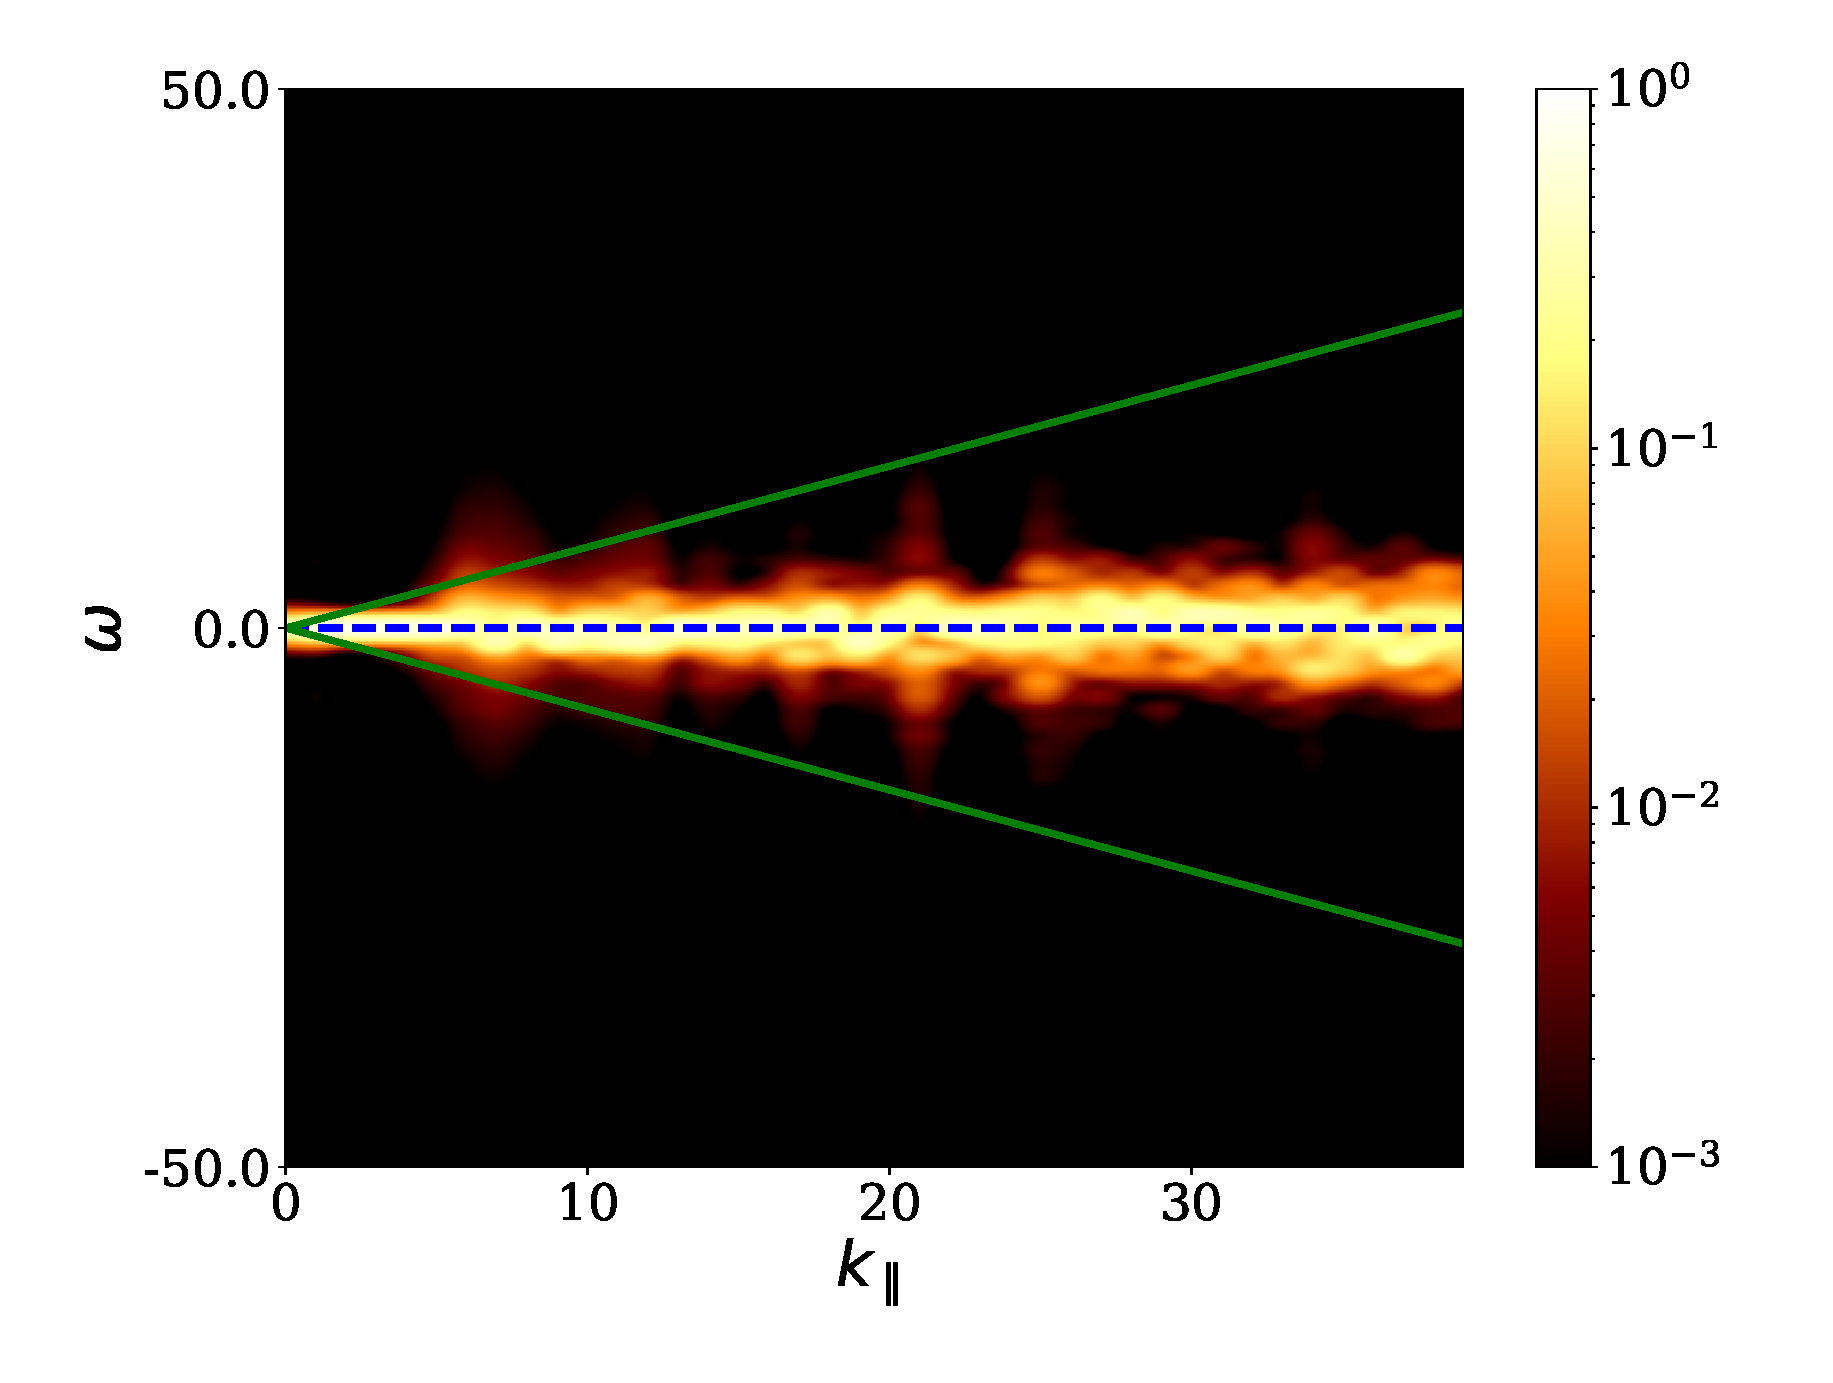
\includegraphics[width=0.45\textwidth]{{CrossHelicity/fig3_B0.0_y_Hc0.9_zp_kperp0}.eps}}
  \caption{Normalized wave vector and frequency spectra
    $E^\pm(\vec{k}, \omega)/E^+(\vec{k})$ of $\vec{z}^-$ (left) and
    $\vec{z}^+$ (right), for the isotropic simulations ($B_0=0$) with
    $\sigma_c = 0.3$ [top, panels (a) and (b)] and $\sigma_c = 0.9$ [bottom,
    panels (c) and (d)], as a function of $k_\parallel$ and for fixed
    $k_\perp=0$. Lighter regions indicate larger energy density. The
    spectra correspond to the power in the time and space Fourier
    transform of the fields, such that accumulation of energy in modes
    near the dispersion relation (or in all modes below the sweeping
    curve) points to a dominance of a physical effect (i.e., of its
    associated frequency) in the dynamics of a given scale
    $\sim 1/k_\parallel$. As a reference, the sweeping time relation
    giving by Eq.~(\ref{eq:tausw}) is indicated by solid (green)
    lines. A broad excitation of modes is observed for all modes with
    $\omega \leq 1/\tau_{sw}$ (sweeping) in panels (a) and (b), and
    for $\omega \approx 0$ in panels (c) and (d).}
  \label{fig3:B0_spectrum_Hc}
\end{figure*}

La condición inicial en todas las simulaciones consistió en amplitudes
no nulas para los campos $\vec{v}(\vec{k})$ y $\vec{b}(\vec{k})$,
equiparticionados en todos los números de onda dentro de los
cascarones con $1.1 \leq k \leq 4$ (en unidades de $2\pi L/\lambda$,
con $\lambda$ la longitud de onda). Se eligieron fases aleatorias para
todos los modos de Fourier en ambos campos.  Para mantener al sistema
en un estado turbulento estacionario, aplicamos forzados $\vec{F}_b$ y
$\vec{F}_v$ para $\vec{b}$ y $\vec{v}$, respectivamente, en las
\cref{eq:MHD_v, eq:MHD_b}). Los forzados $\vec{F}_b$ y $\vec{F}_v$ se
encuentran limitados a una banda fija de modos de Fourier,
$0.9\leq k \leq 1.8$. El forzado tiene una componente aleatoria y una
coherente temporalmente, con un tiempo de correlación del forzado de
$\tau_f \approx 1$ (del orden de la unidad de tiempo $t_0$), que es
mayor que todos los tiempos característicos definidos en la sección
anterior.  Para cambiar el nivel de helicidad cruzada en el flujo, se
introdujeron correlaciones entre los forzados mecánico y magnético,
resultando a tiempos altos (dependiendo del nivel de correlación
cruzada entre los forzados) en una correlación cruzada normalizada de
$\sigma_c=0$, $0.3$, o $0.9$. Estos valores corresponden al promedio
temporal en el estado turbulento estacionario; en la práctica, cada
simulación tiene una helicidad cruzada instantánea que fluctúa en el
tiempo alrededor de los valores medios reportados.

Notar los diferentes valores de $B_0$ y de $\sigma_c$ explorados,
resultando en un total de 18 simulaciones. Todas las simulaciones
fueron realizadas hasta que el sistema alcanzase un estado turbulento
estacionario, y luego fueron continuadas para realizar el análisis
espacio-temporal de la evolución de los campos de Els\"asser
presentados en la próxima sección. No obstante, primero caracterizamos
el comportamiento espacial de los flujos (considerando especialmente
el grado de anisotropía a medida que se aumentaba la intensidad del
campo de fondo), para luego estudiar en comportamiento de las
fluctuaciones de Els\"asser utilizando la información
espacio-temporal.

\section{Results}\label{sec_results}

\begin{figure*}
  \centering
  \subfigure[$B_0 = 0.25$, $\vec{z}^-$, $\sigma_c = 0$]{\includegraphics[width=0.45\textwidth]{{CrossHelicity/fig3_B0.25_y_Hc0.0_zm_kperp0}.eps}}
  \subfigure[$B_0 = 0.25$, $\vec{z}^+$, $\sigma_c = 0$]{\includegraphics[width=0.45\textwidth]{{CrossHelicity/fig3_B0.25_y_Hc0.0_zp_kperp0}.eps}}
  \subfigure[$B_0 = 0.25$, $\vec{z}^-$, $\sigma_c = 0.3$]{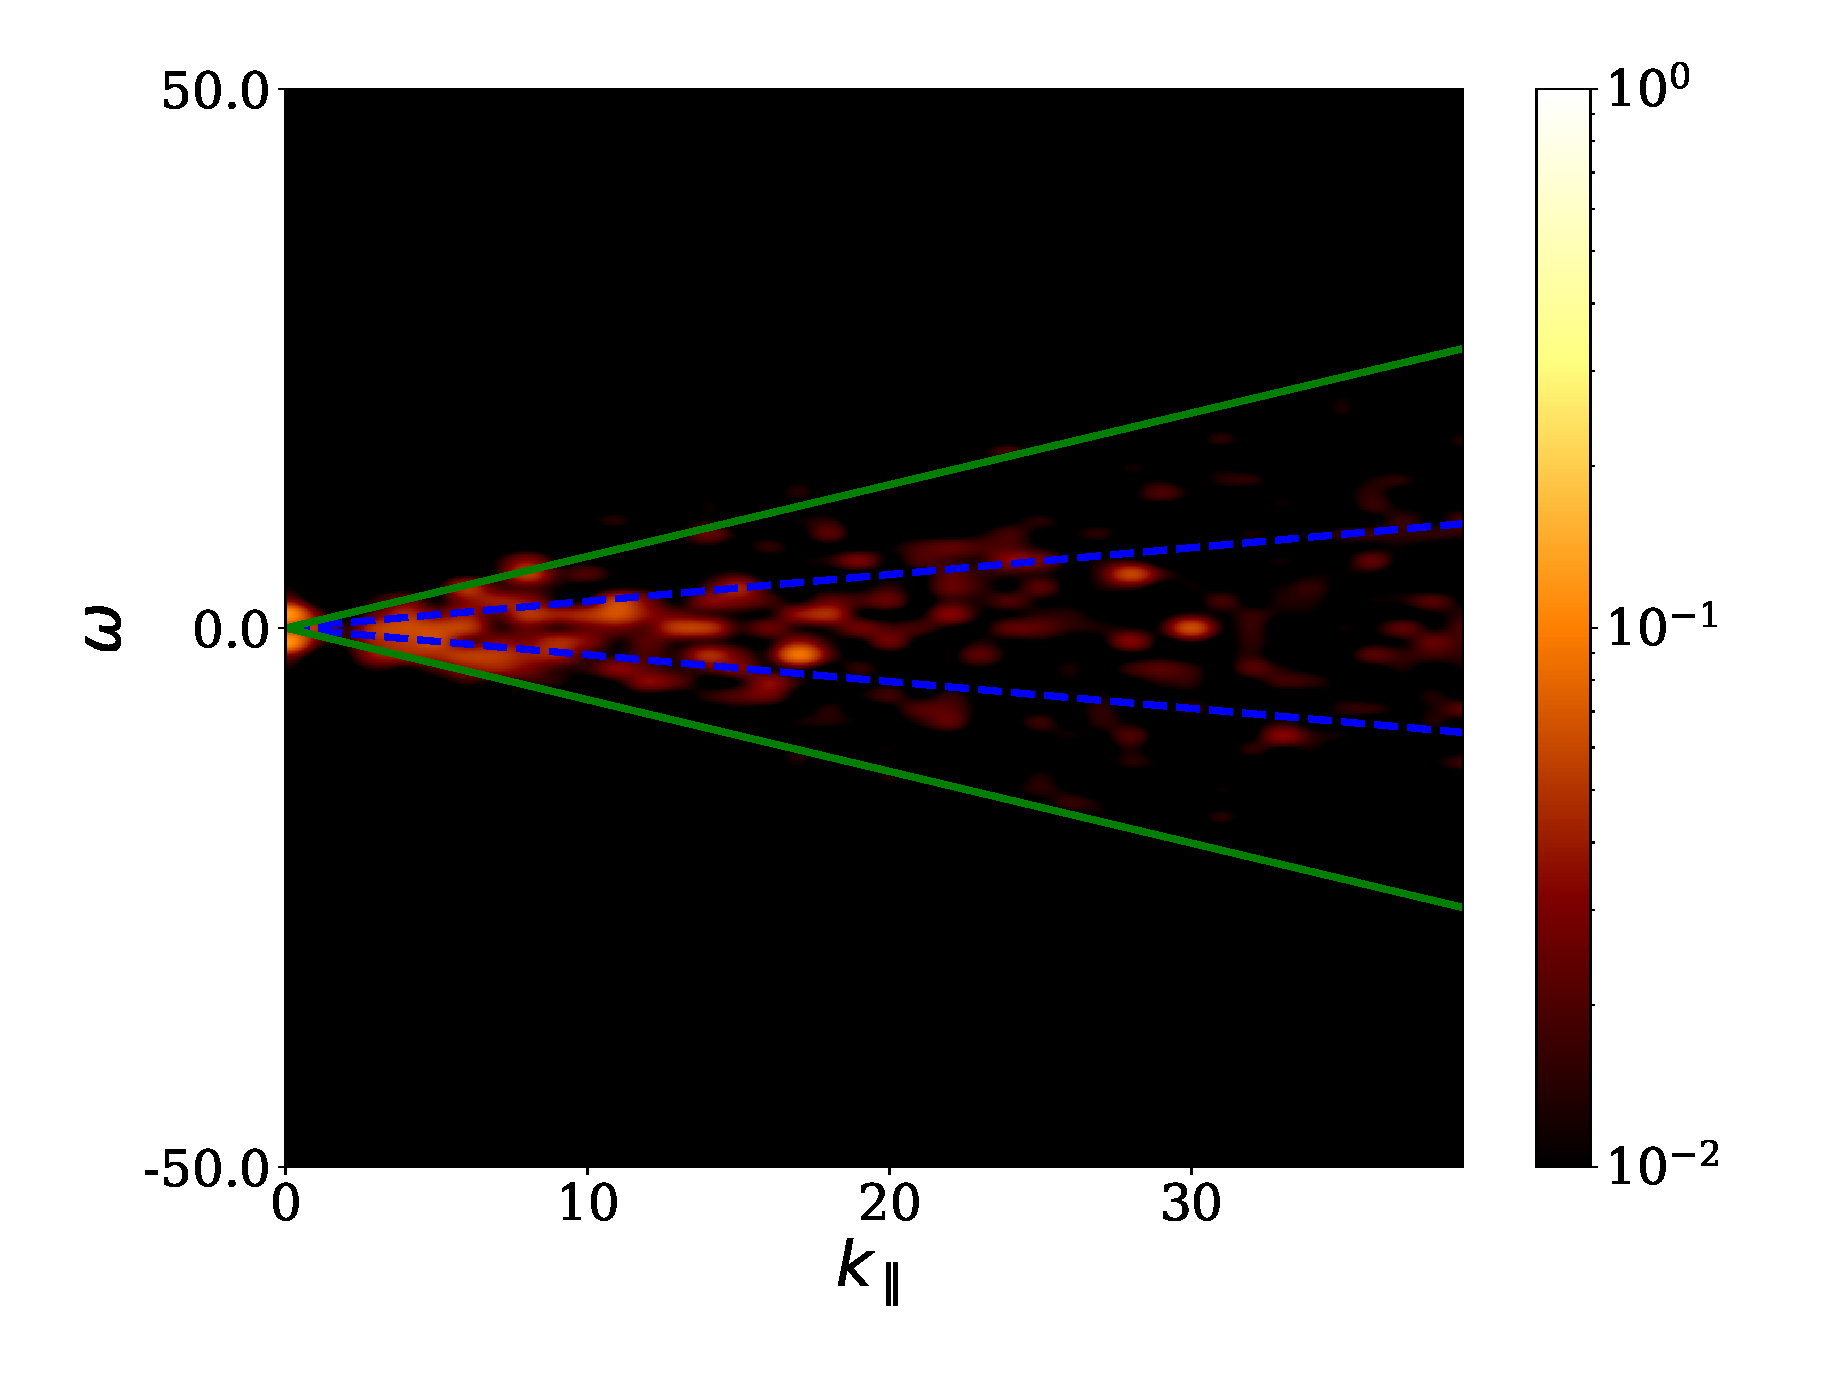
\includegraphics[width=0.45\textwidth]{{CrossHelicity/fig3_B0.25_y_Hc0.3_zm_kperp0}.eps}}
  \subfigure[$B_0 = 0.25$, $\vec{z}^+$, $\sigma_c = 0.3$]{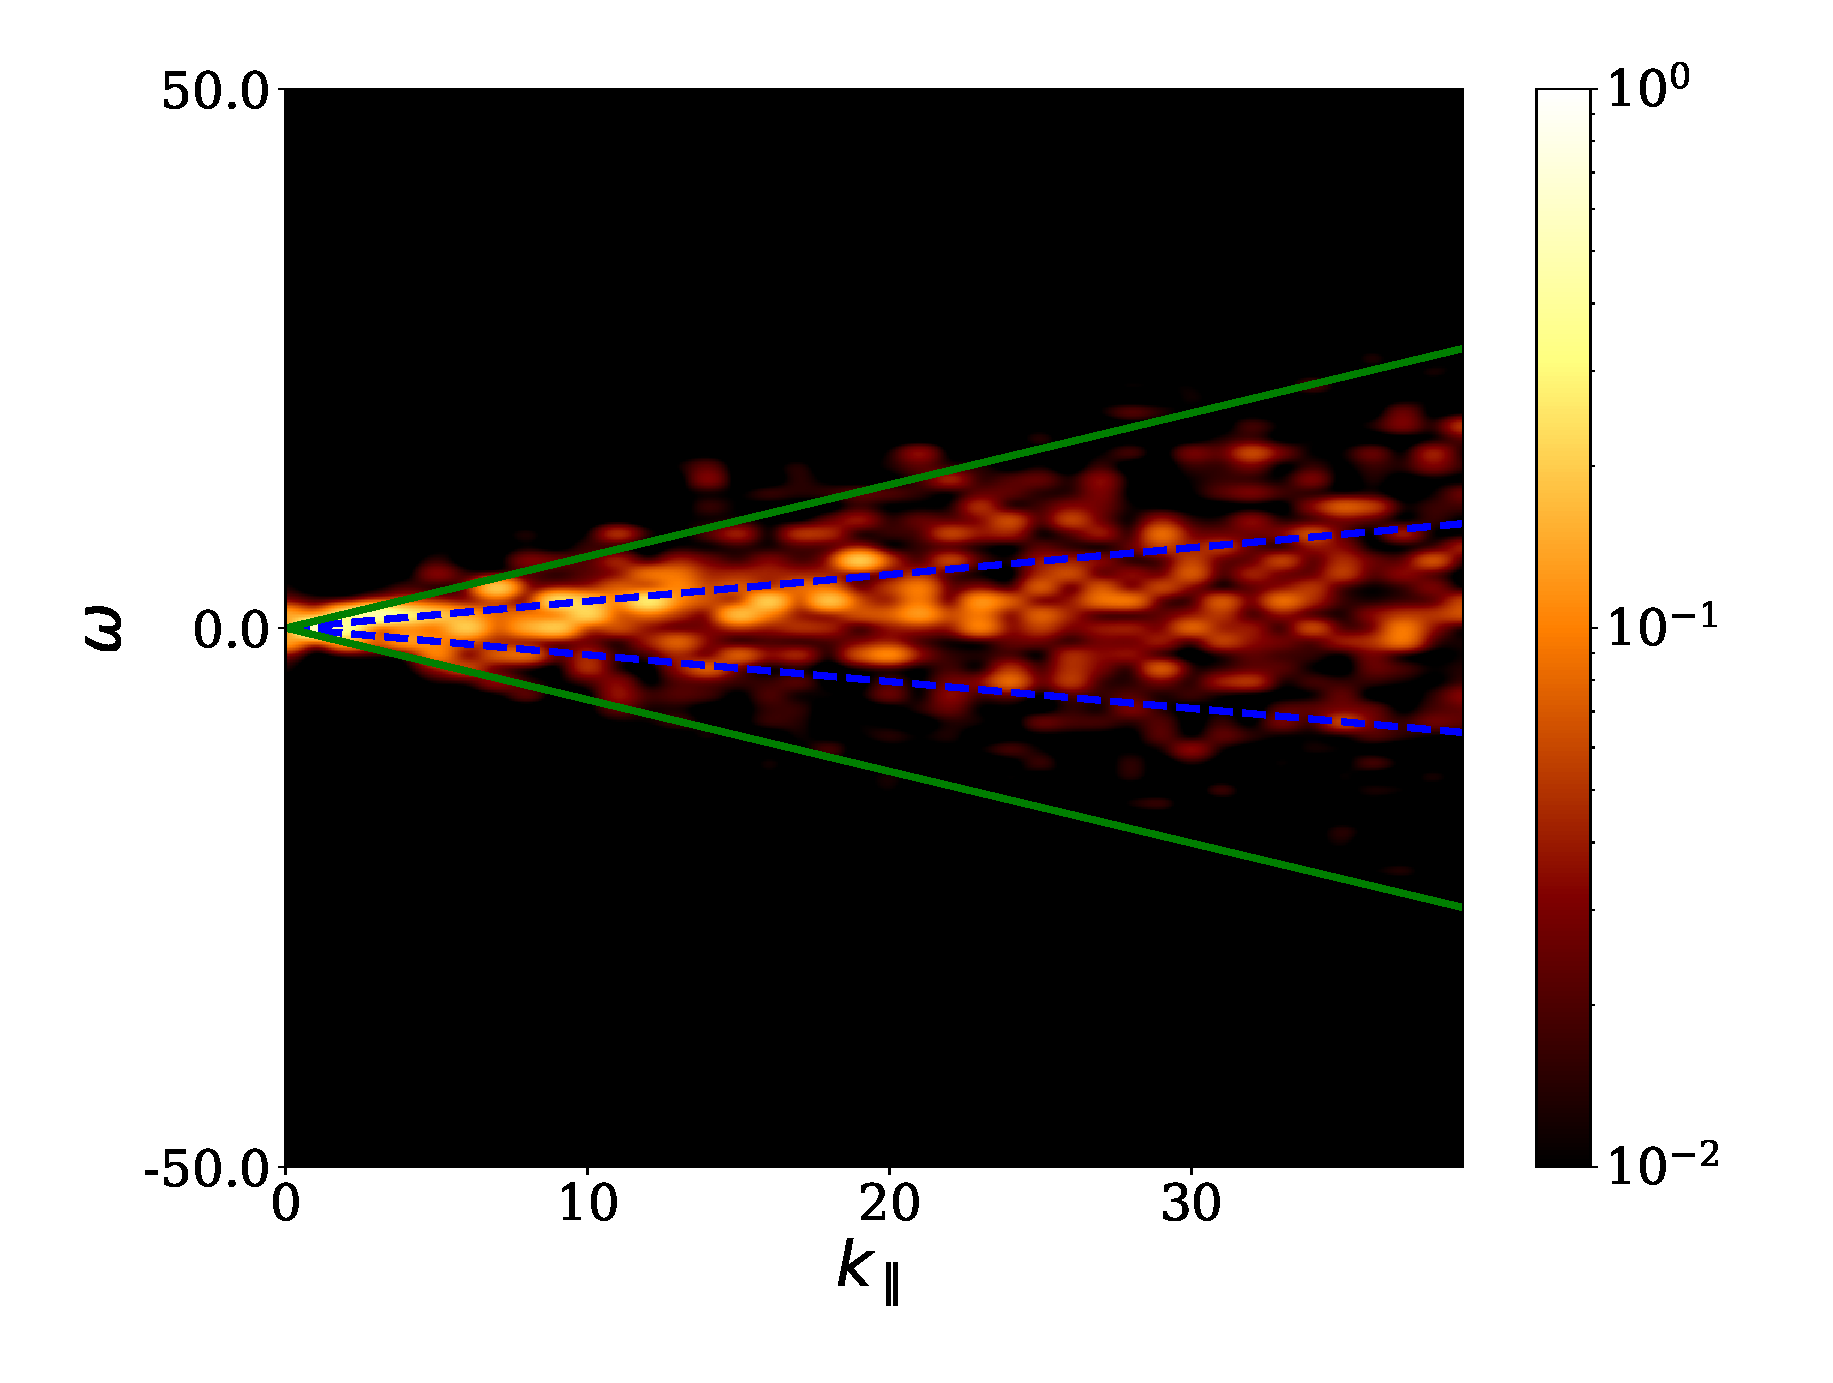
\includegraphics[width=0.45\textwidth]{{CrossHelicity/fig3_B0.25_y_Hc0.3_zp_kperp0}.eps}}
  \subfigure[$B_0 = 0.25$, $\vec{z}^-$, $\sigma_c = 0.9$]{\includegraphics[width=0.45\textwidth]{{CrossHelicity/fig3_B0.25_y_Hc0.9_zm_kperp0}.eps}}
  \subfigure[$B_0 = 0.25$, $\vec{z}^+$, $\sigma_c = 0.9$]{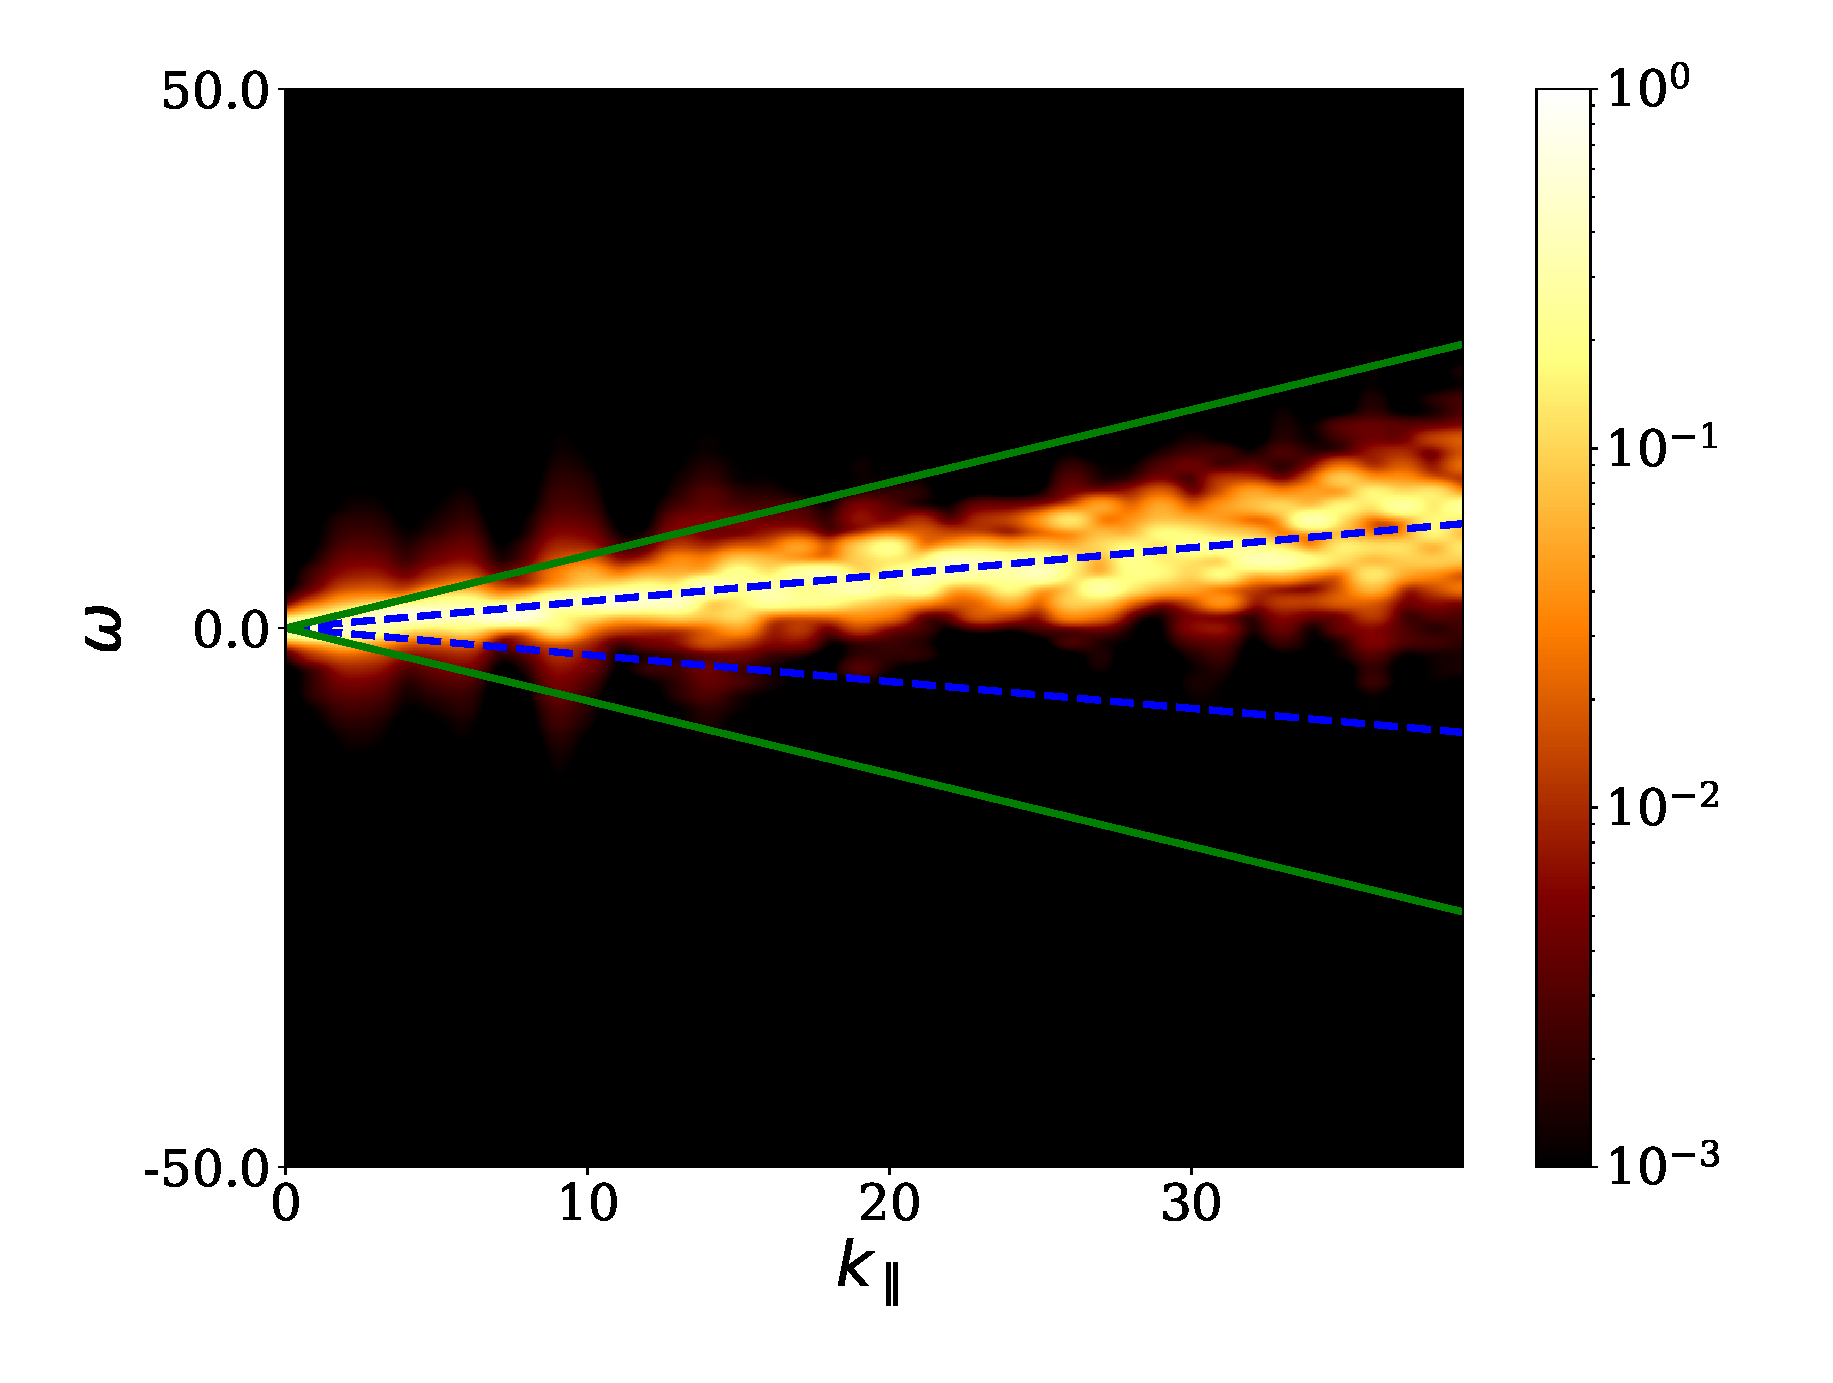
\includegraphics[width=0.45\textwidth]{{CrossHelicity/fig3_B0.25_y_Hc0.9_zp_kperp0}.eps}}
    \caption{Normalized spectra $E^\pm(\vec{k}, \omega)/E^+(\vec{k})$ of $\vec{z}^-$ (left)
    and $\vec{z}^+$ (right), for the runs with $B_0=0.25$, for modes with $k_\perp=0$, and 
    thus as a function of $k_\parallel$ and $\omega$. Panels (a) and (b) correspond to 
    $\sigma_c = 0$, (c) and (d) to $\sigma_c = 0.3$, and (e) and (f) to $\sigma_c = 0.9$. 
    The sweeping time relation, given by Eq.~(\ref{eq:tausw}), is indicated by solid (green)
    lines, and the dashed (blue) lines indicate the dispersion relation of Alfv\'en waves. 
    Lighter regions indicate larger energy density, and the accumulation of energy in modes
    near the dispersion relation (or in all modes below the sweeping curve) points to a 
    dominance of a physical effect (i.e., of its associated frequency) in the dynamics of a 
    given scale $\sim 1/k_\parallel$. For low normalized cross-helicity $\sigma_c$ sweeping is the dominant effect, while for large $\sigma_c$ energy accumulates near the dispersion relation 
    of the waves, albeit for both $\vec{z}^+$ and $\vec{z}^-$ with the same sign of the frequency $\omega$.}
  \label{fig3:B025_spectrum_Hc}
\end{figure*}

\begin{figure*}
  \centering
  \subfigure[$B_0 = 1.0$, $\vec{z}^-$, $\sigma_c = 0$]{\includegraphics[width=0.45\textwidth]{{CrossHelicity/fig3_B1.0_y_Hc0.0_zm_kperp0}.eps}}
  \subfigure[$B_0 = 1.0$, $\vec{z}^+$, $\sigma_c = 0$]{\includegraphics[width=0.45\textwidth]{{CrossHelicity/fig3_B1.0_y_Hc0.0_zp_kperp0}.eps}}
  \subfigure[$B_0 = 1.0$, $\vec{z}^-$, $\sigma_c = 0.3$]{\includegraphics[width=0.45\textwidth]{{CrossHelicity/fig3_B1.0_y_Hc0.3_zm_kperp0}.eps}}
  \subfigure[$B_0 = 1.0$, $\vec{z}^+$, $\sigma_c = 0.3$]{\includegraphics[width=0.45\textwidth]{{CrossHelicity/fig3_B1.0_y_Hc0.3_zp_kperp0}.eps}}
  \subfigure[$B_0 = 1.0$, $\vec{z}^-$, $\sigma_c = 0.9$]{\includegraphics[width=0.45\textwidth]{{CrossHelicity/fig3_B1.0_y_Hc0.9_zm_kperp0}.eps}}
  \subfigure[$B_0 = 1.0$, $\vec{z}^+$, $\sigma_c = 0.9$]{\includegraphics[width=0.45\textwidth]{{CrossHelicity/fig3_B1.0_y_Hc0.9_zp_kperp0}.eps}}
    \caption{Normalized spectra $E^\pm(\vec{k}, \omega)/E^+(\vec{k})$ of $\vec{z}^-$ (left) and $\vec{z}^+$ (right), for the runs with $B_0=1$, for modes with $k_\perp=0$, and thus as a function of $k_\parallel$ and $\omega$. Panels (a) and (b) correspond to $\sigma_c = 0$, (c) and (d) to $\sigma_c = 0.3$, and (e) and (f) to $\sigma_c = 0.9$. The sweeping time relation, given by Eq.~(\ref{eq:tausw}), is indicated by solid (green)
    lines, and the dashed (blue) lines indicate the dispersion relation of Alfv\'en waves. Lighter regions indicate larger energy density. In this case power for $\sigma_c = 0$ is concentrated in a region near the wave dispersion relations $\omega^\pm \approx \pm \vec{V}_\textrm{A}\cdot\vec{k}$ up to $k_\parallel \approx 10$. For $\sigma_c = 0.9$, both fields $\vec{z}^+$ and $\vec{z}^-$ follow the same dispersion relation $\omega \approx + \vec{V}_\textrm{A}\cdot\vec{k}$, and Alfv\'enic excitations dominate over all scales.}
  \label{fig3:B1_spectrum_Hc}
\end{figure*}

\begin{figure*}
  \centering
  \subfigure[$B_0 = 8.0$, $\vec{z}^-$, $\sigma_c = 0$]{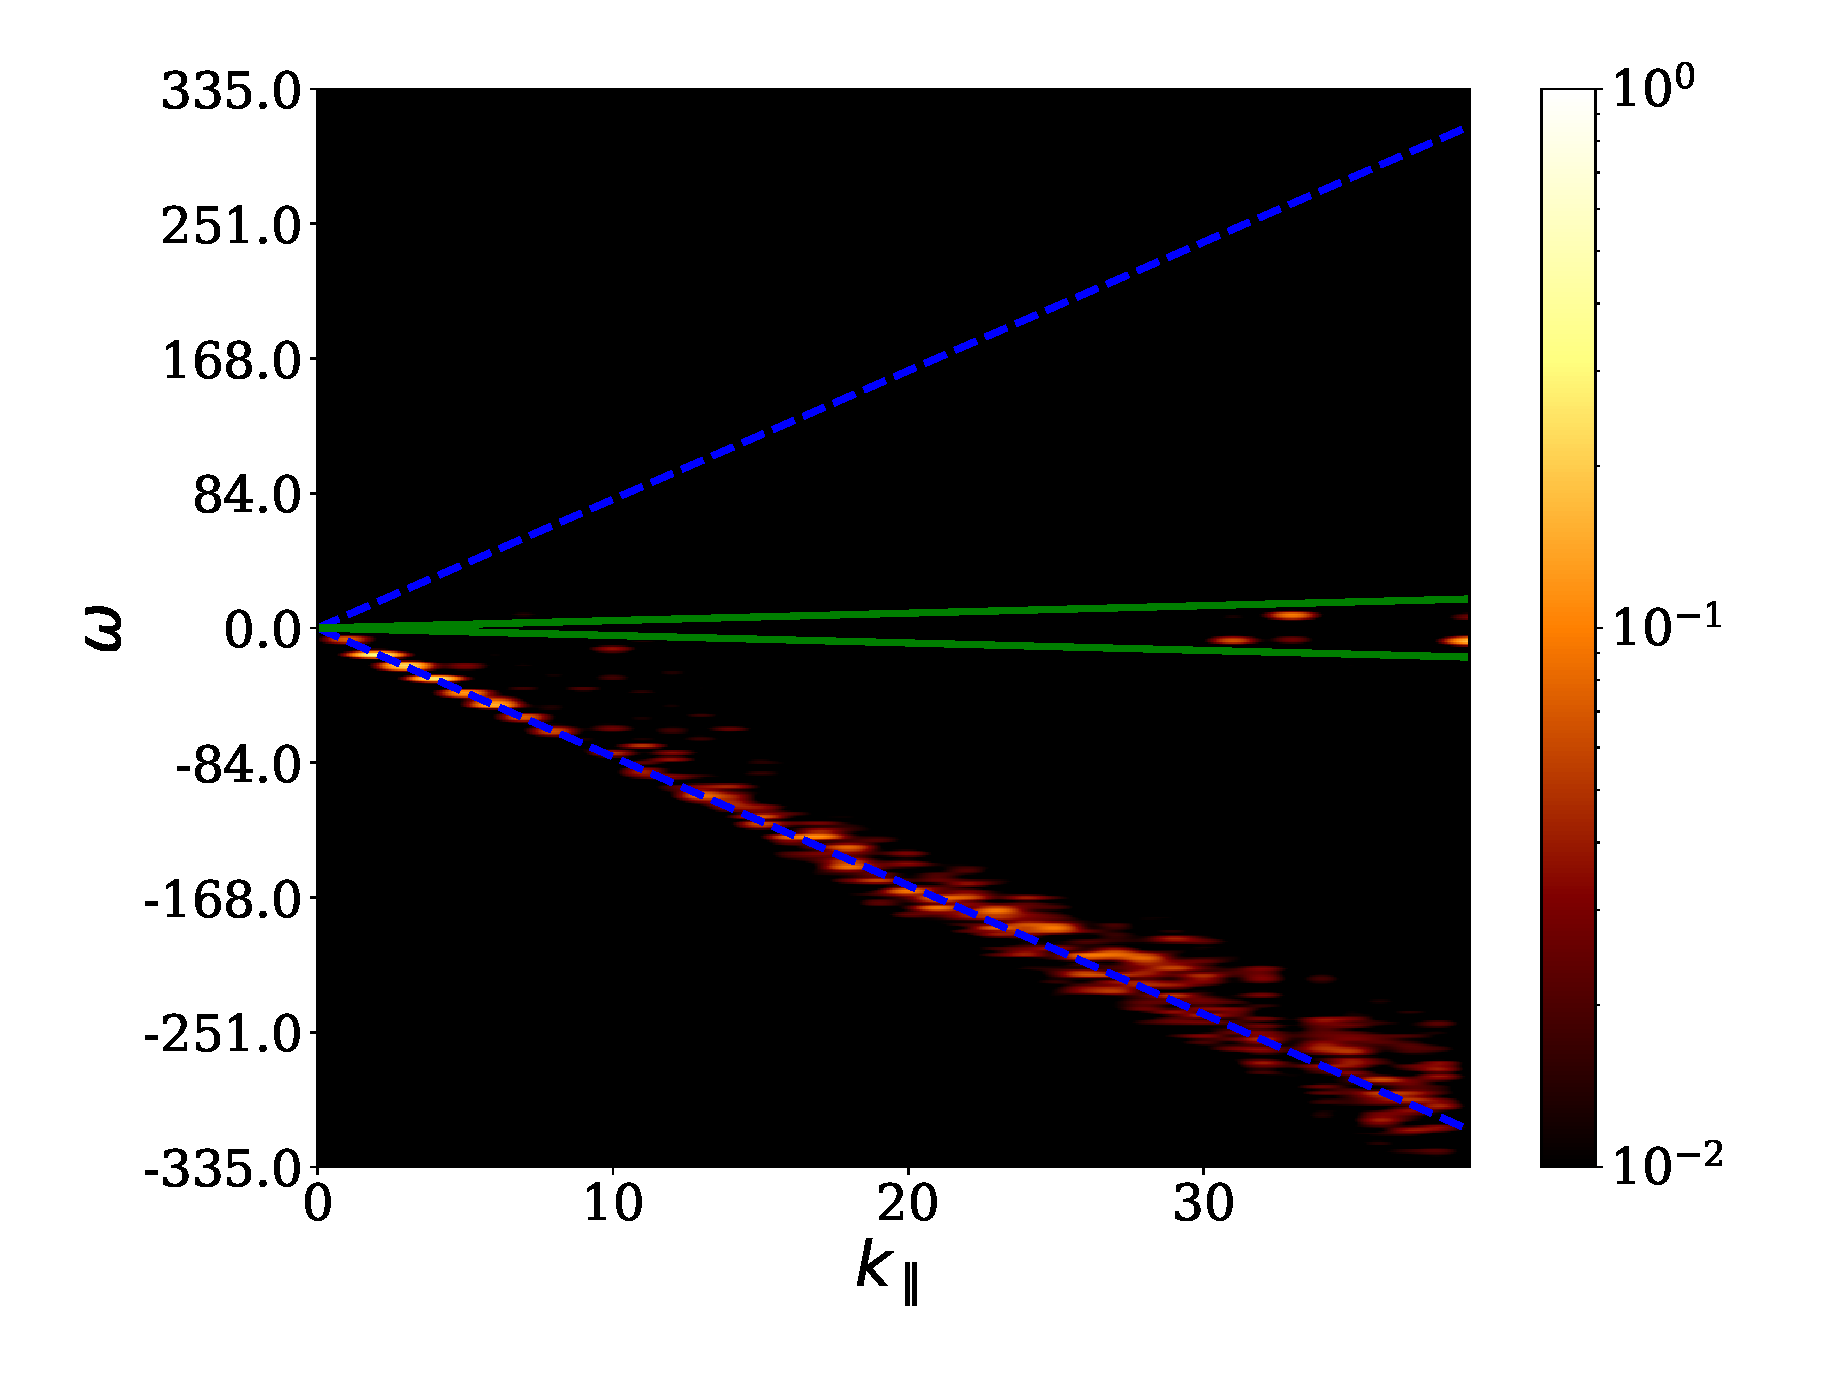
\includegraphics[width=0.45\textwidth]{{CrossHelicity/fig3_B8.0_y_Hc0.0_zm_kperp0}.eps}}
  \subfigure[$B_0 = 8.0$, $\vec{z}^+$, $\sigma_c = 0$]{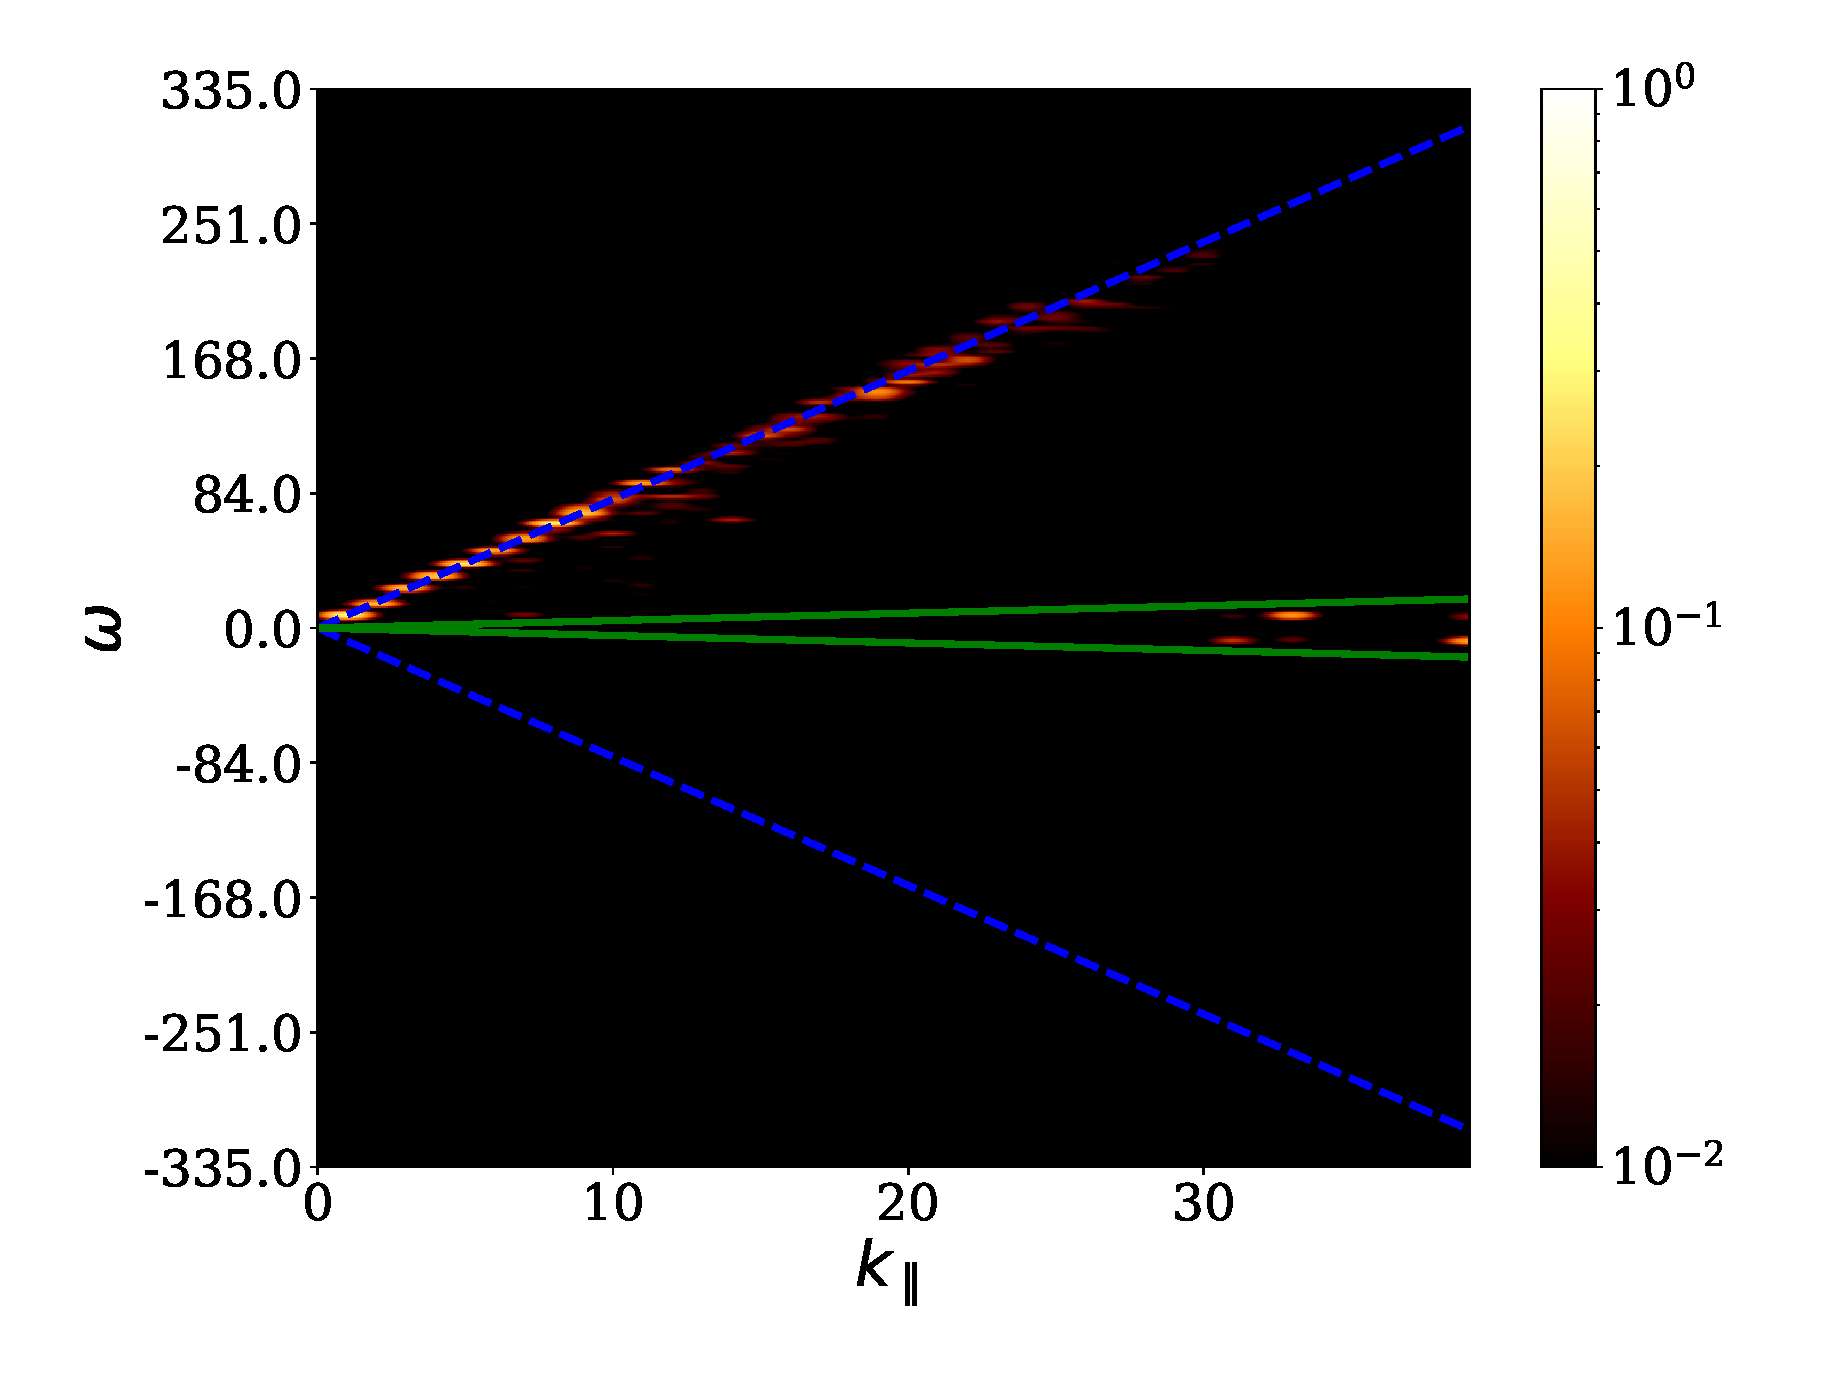
\includegraphics[width=0.45\textwidth]{{CrossHelicity/fig3_B8.0_y_Hc0.0_zp_kperp0}.eps}}
  \subfigure[$B_0 = 8.0$, $\vec{z}^-$, $\sigma_c = 0.3$]{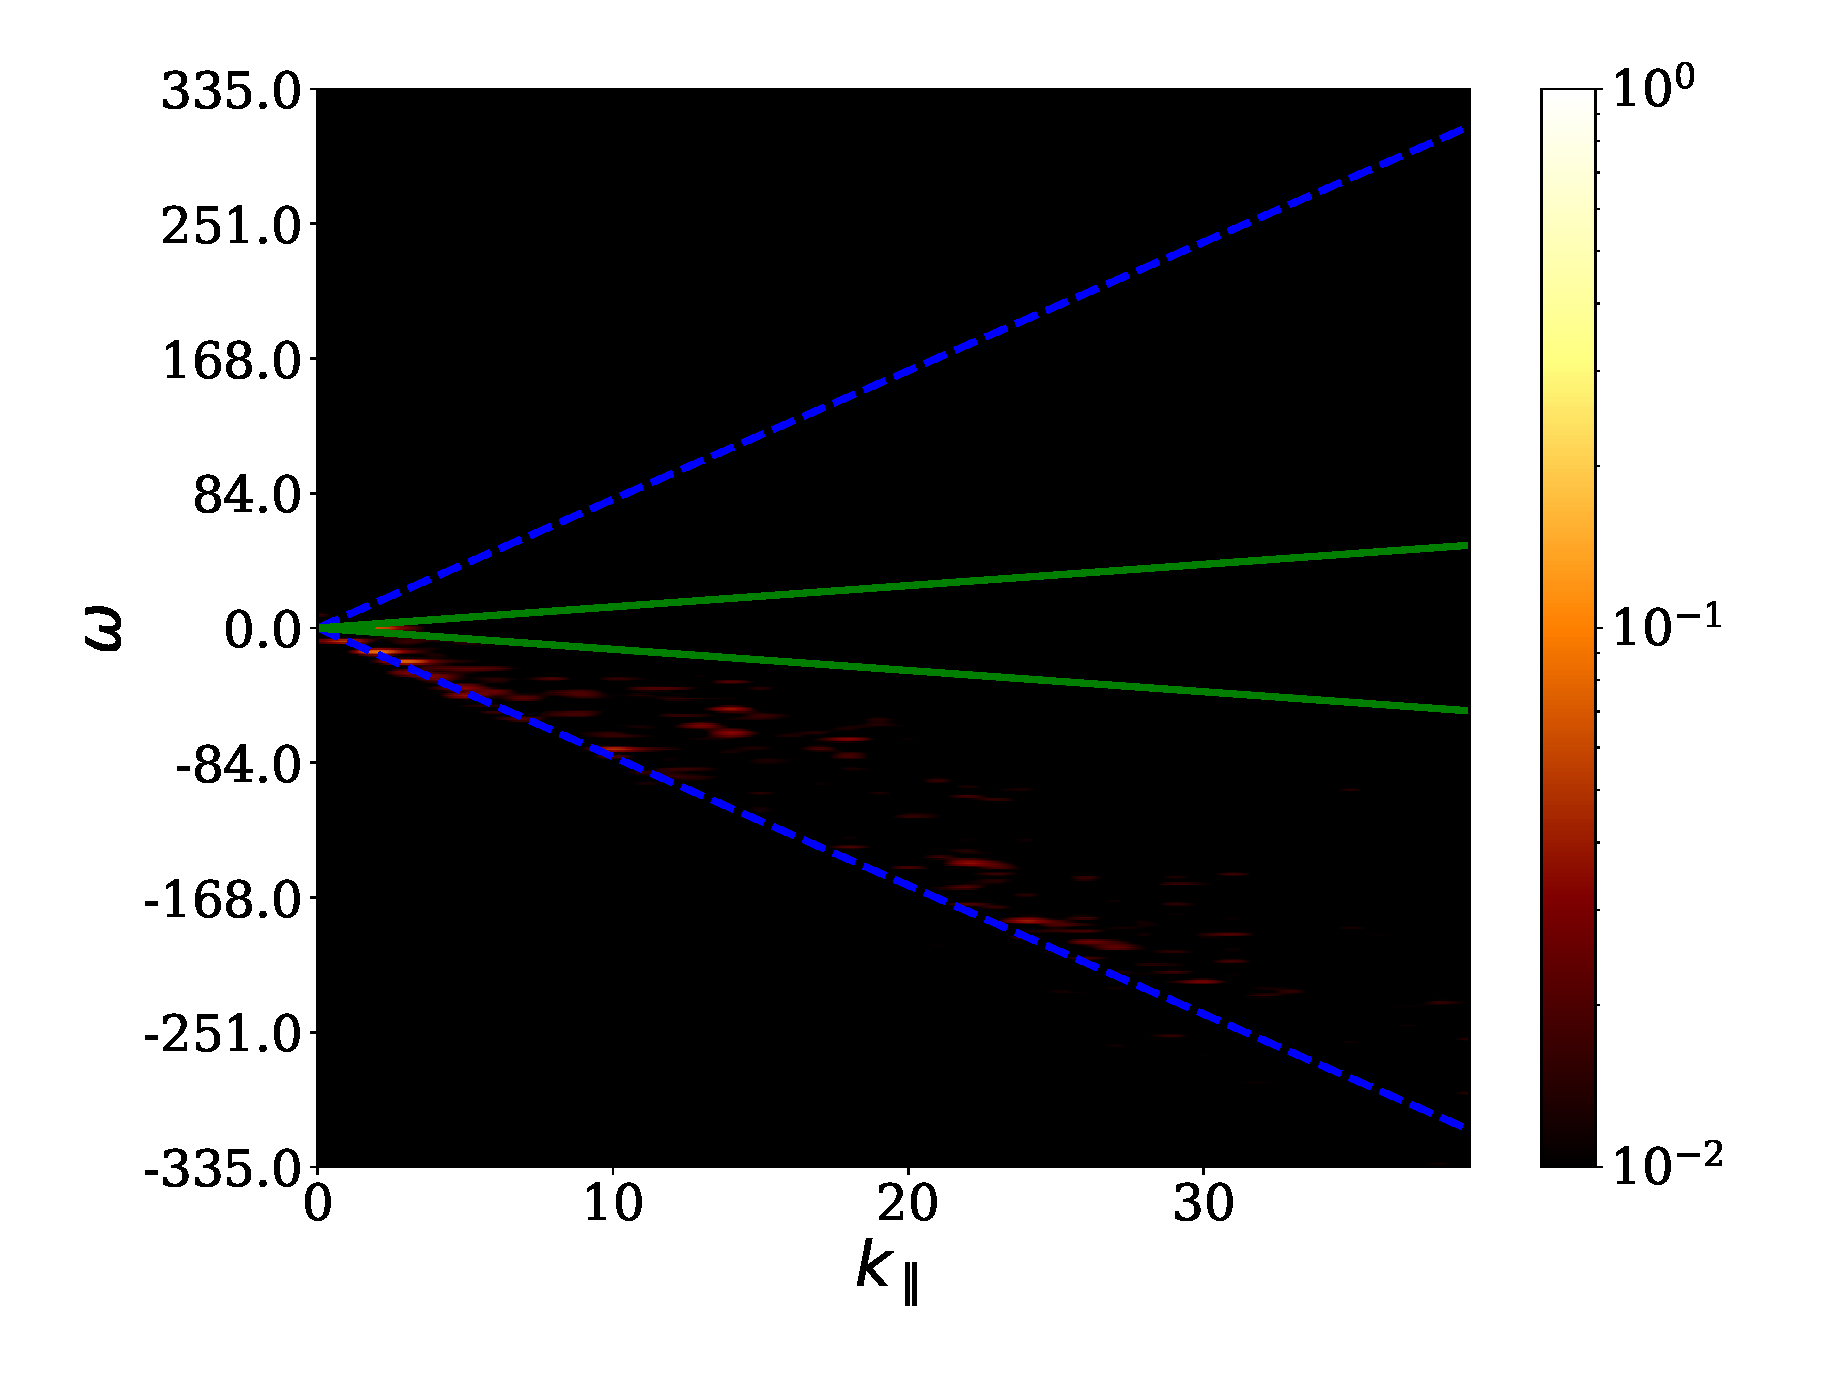
\includegraphics[width=0.45\textwidth]{{CrossHelicity/fig3_B8.0_y_Hc0.3_zm_kperp0}.eps}}
  \subfigure[$B_0 = 8.0$, $\vec{z}^+$, $\sigma_c = 0.3$]{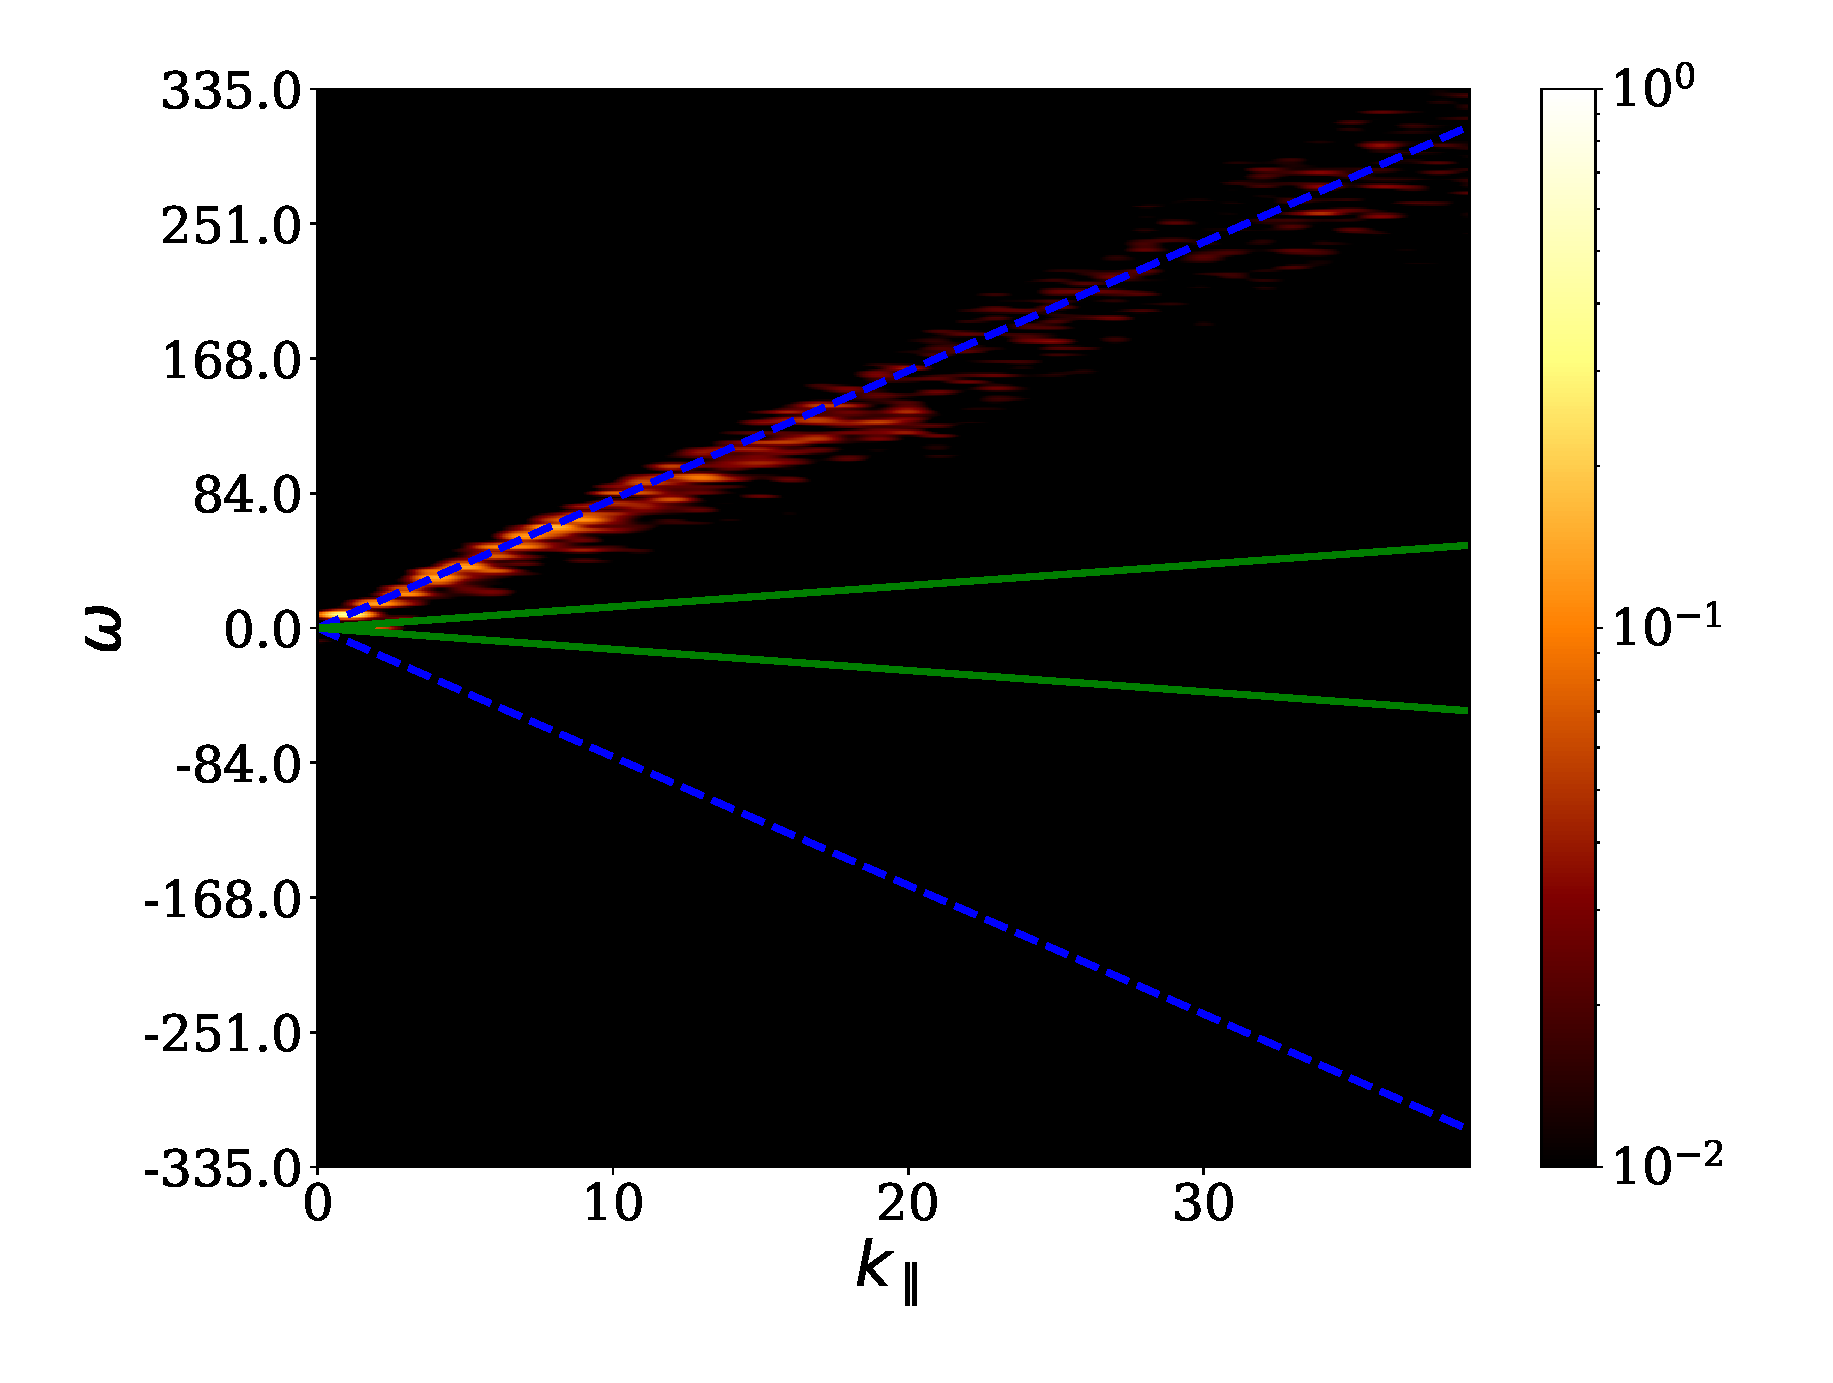
\includegraphics[width=0.45\textwidth]{{CrossHelicity/fig3_B8.0_y_Hc0.3_zp_kperp0}.eps}}
  \subfigure[$B_0 = 8.0$, $\vec{z}^-$, $\sigma_c = 0.9$]{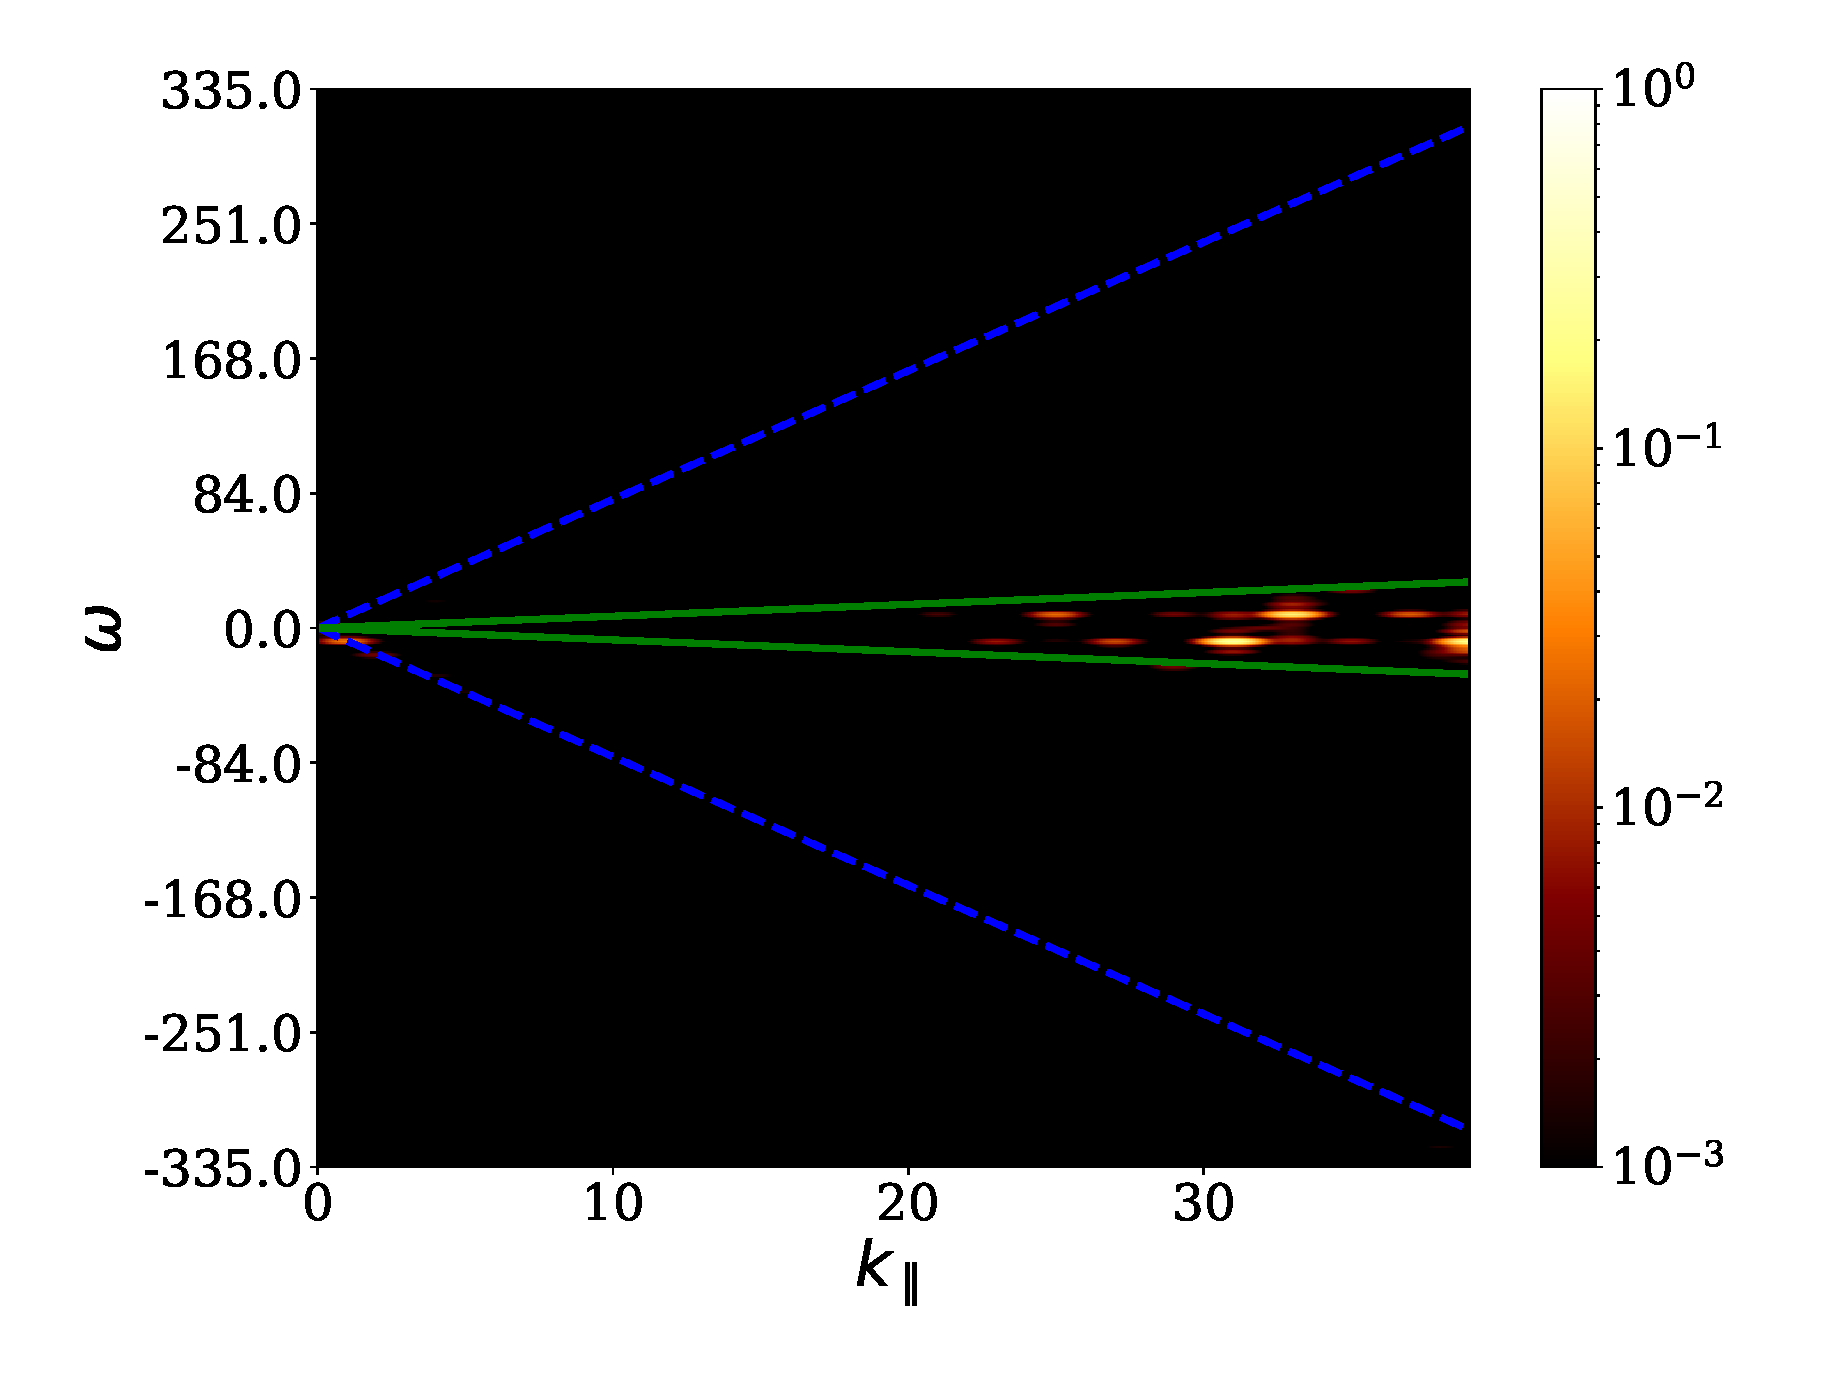
\includegraphics[width=0.45\textwidth]{{CrossHelicity/fig3_B8.0_y_Hc0.9_zm_kperp0}.eps}}
  \subfigure[$B_0 = 8.0$, $\vec{z}^+$, $\sigma_c = 0.9$]{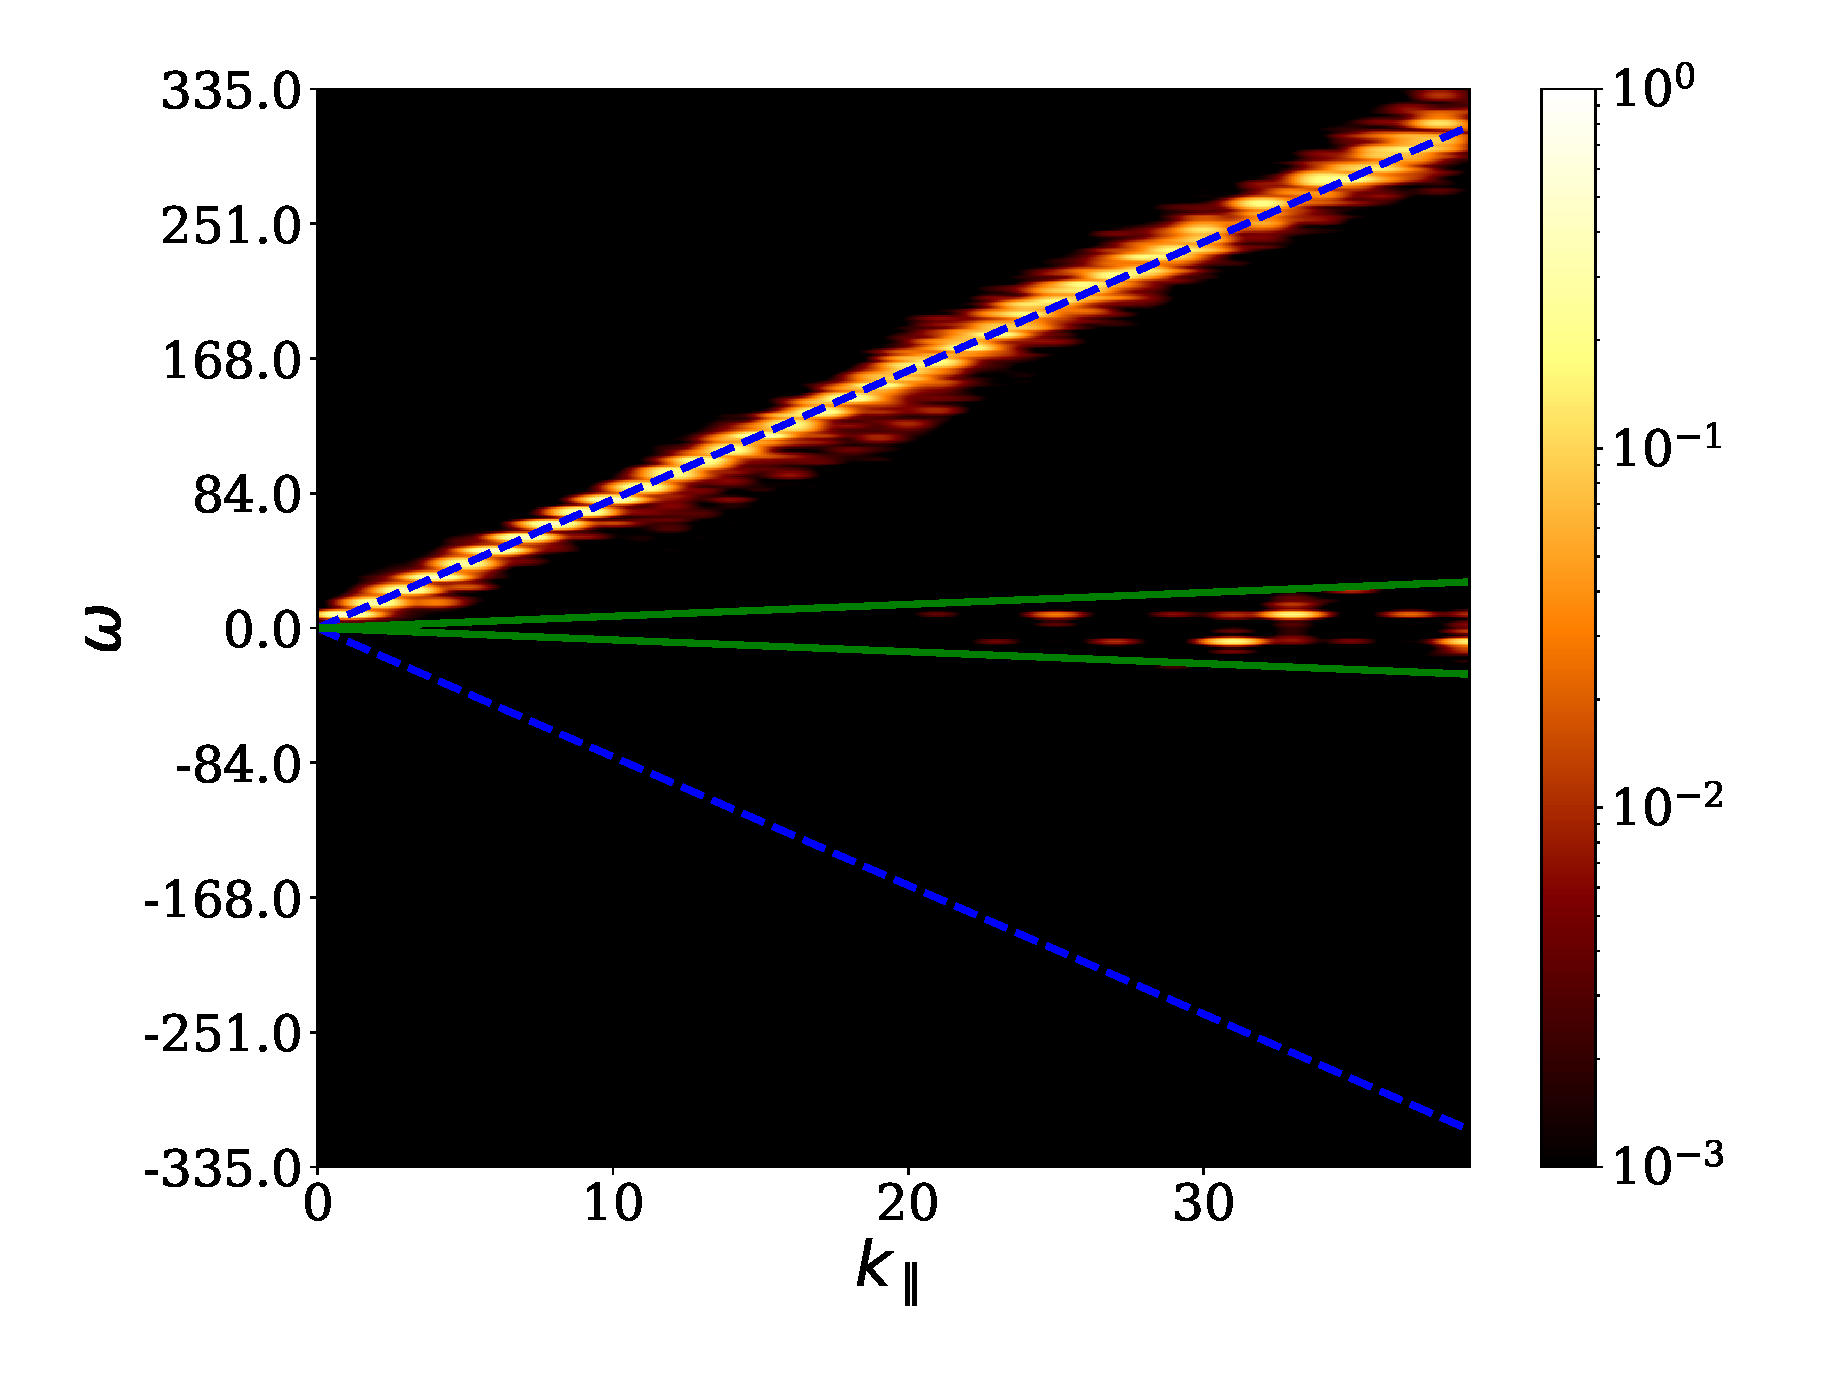
\includegraphics[width=0.45\textwidth]{{CrossHelicity/fig3_B8.0_y_Hc0.9_zp_kperp0}.eps}}
  \caption{Normalized spectra $E^\pm(\vec{k}, \omega)/E^+(\vec{k})$ of
    $\vec{z}^-$ (left) and $\vec{z}^+$ (right), for the runs with
    $B_0=8$, for modes with $k_\perp=0$, and thus as a function of
    $k_\parallel$ and $\omega$. Panels (a) and (b) correspond to
    $\sigma_c = 0$, (c) and (d) to $\sigma_c = 0.3$, and (e) and (f)
    to $\sigma_c = 0.9$. The sweeping time relation, given by
    Eq.~(\ref{eq:tausw}), is indicated by solid (green) lines, and the
    dashed (blue) lines indicate the dispersion relation of Alfv\'en
    waves. Lighter regions indicate larger energy density. In all
    cases power is concentrated in a narrow region near the wave
    dispersion relations
    $\omega^\pm \approx \pm \vec{V}_\textrm{A}\cdot\vec{k}$ or near
    $\omega \approx 0$, for all the wavenumbers studied, and there is
    no evidence of counter-propagation of waves.}
  \label{fig3:B8_spectrum_Hc}
\end{figure*}

\subsection{Wavenumber spectra}

Luego de que el sistema alcanzase un estado turbulento estacionario,
analizamos todos los resultados durante al menos $10$ unidades
temporales de gran escala, luego de verificar que esta cantidad de
tiempo era suficiente para que convergieran los espectros
espacio-temporales y las funciones de correlación.

Comenzamos la discusión con el espectro espacial, para caracterizas la
turbulencia y para cuantificar su anisotropía a medida que se varía la
intensidad del campo guía, para diferentes valores de la helicidad
cruzada.  Los espectros energéticos perpendiculares reducidos
$E(k_\perp)$ se muestran en la \cref{fig1:E} para las simulaciones con
$B_0=0$, $0.25$, $1$, $2$, $4$, y $8$ con helicidad cruzada
normalizada $\sigma_c=0.3$. Las simulaciones con $\sigma_c=0$ y
$\sigma_c=0.9$ muestran un comportamiento similar.  También se muestra
una ley de potencias tipo Kolmogorov como referencia. Como se puede
ver, a pesar de la resolución espacial moderada de las corridas, los
espectros espaciales observados son compatibles con el escaleo de
Kolmogorov $\sim k_\perp^{-5/3}$, y las simulaciones está bien
resueltas, mostrando el rango disipativo para los números de onda más
grandes (por ejemplo, las escalas de disipación de Kolmogorov $k_\nu$
son $k_\nu \approx 91$, $152$, y $122$ para las simulaciones con
$B_0 = 1$ y $\sigma_c = 0$, $0.3$, y $0.9$ respectivamente).

Se puede ver una ilustración más detallada del comportamiento
espectral (y de la anisotropía de los flujos) en la
\cref{fig2:isocontourns}. Ahí, mostramos los isocontornos del espectro
energético axisimétrico $e(k_\perp, k_\parallel)$ (i.e., la densidad
energética en función de los números de onda perpendicular y paralelo)
para $B_0=0$, $1$, $4$, y $8$, y en todos los casos para flujos con
$\sigma_c = 0.3$. Como referencia, también se indican las curvas (en
el espacio de Fourier) donde el tiempo de Alfvén es igual a o bien el
tiempo de \sweeping, o bien al tiempo no lineal.  En otras palabras,
estas curvas separan regiones en las que (a partir de argumentos
teóricos) la escala temporal más rápida puede esperarse que sea o bien
$\tau_A$ (sobre la línea rayada roja) o bien $\tau_{nl}$ (debajo de la
línea sólida azul). El tiempo de \sweeping puede ser relevante para
todos los modos debajo de la línea rayada roja.

\begin{figure}
  \centering
  \subfigure[$\vec{z}^-$, $B_0=1$, $\sigma_c=0.3$, $k_\parallel=10$]{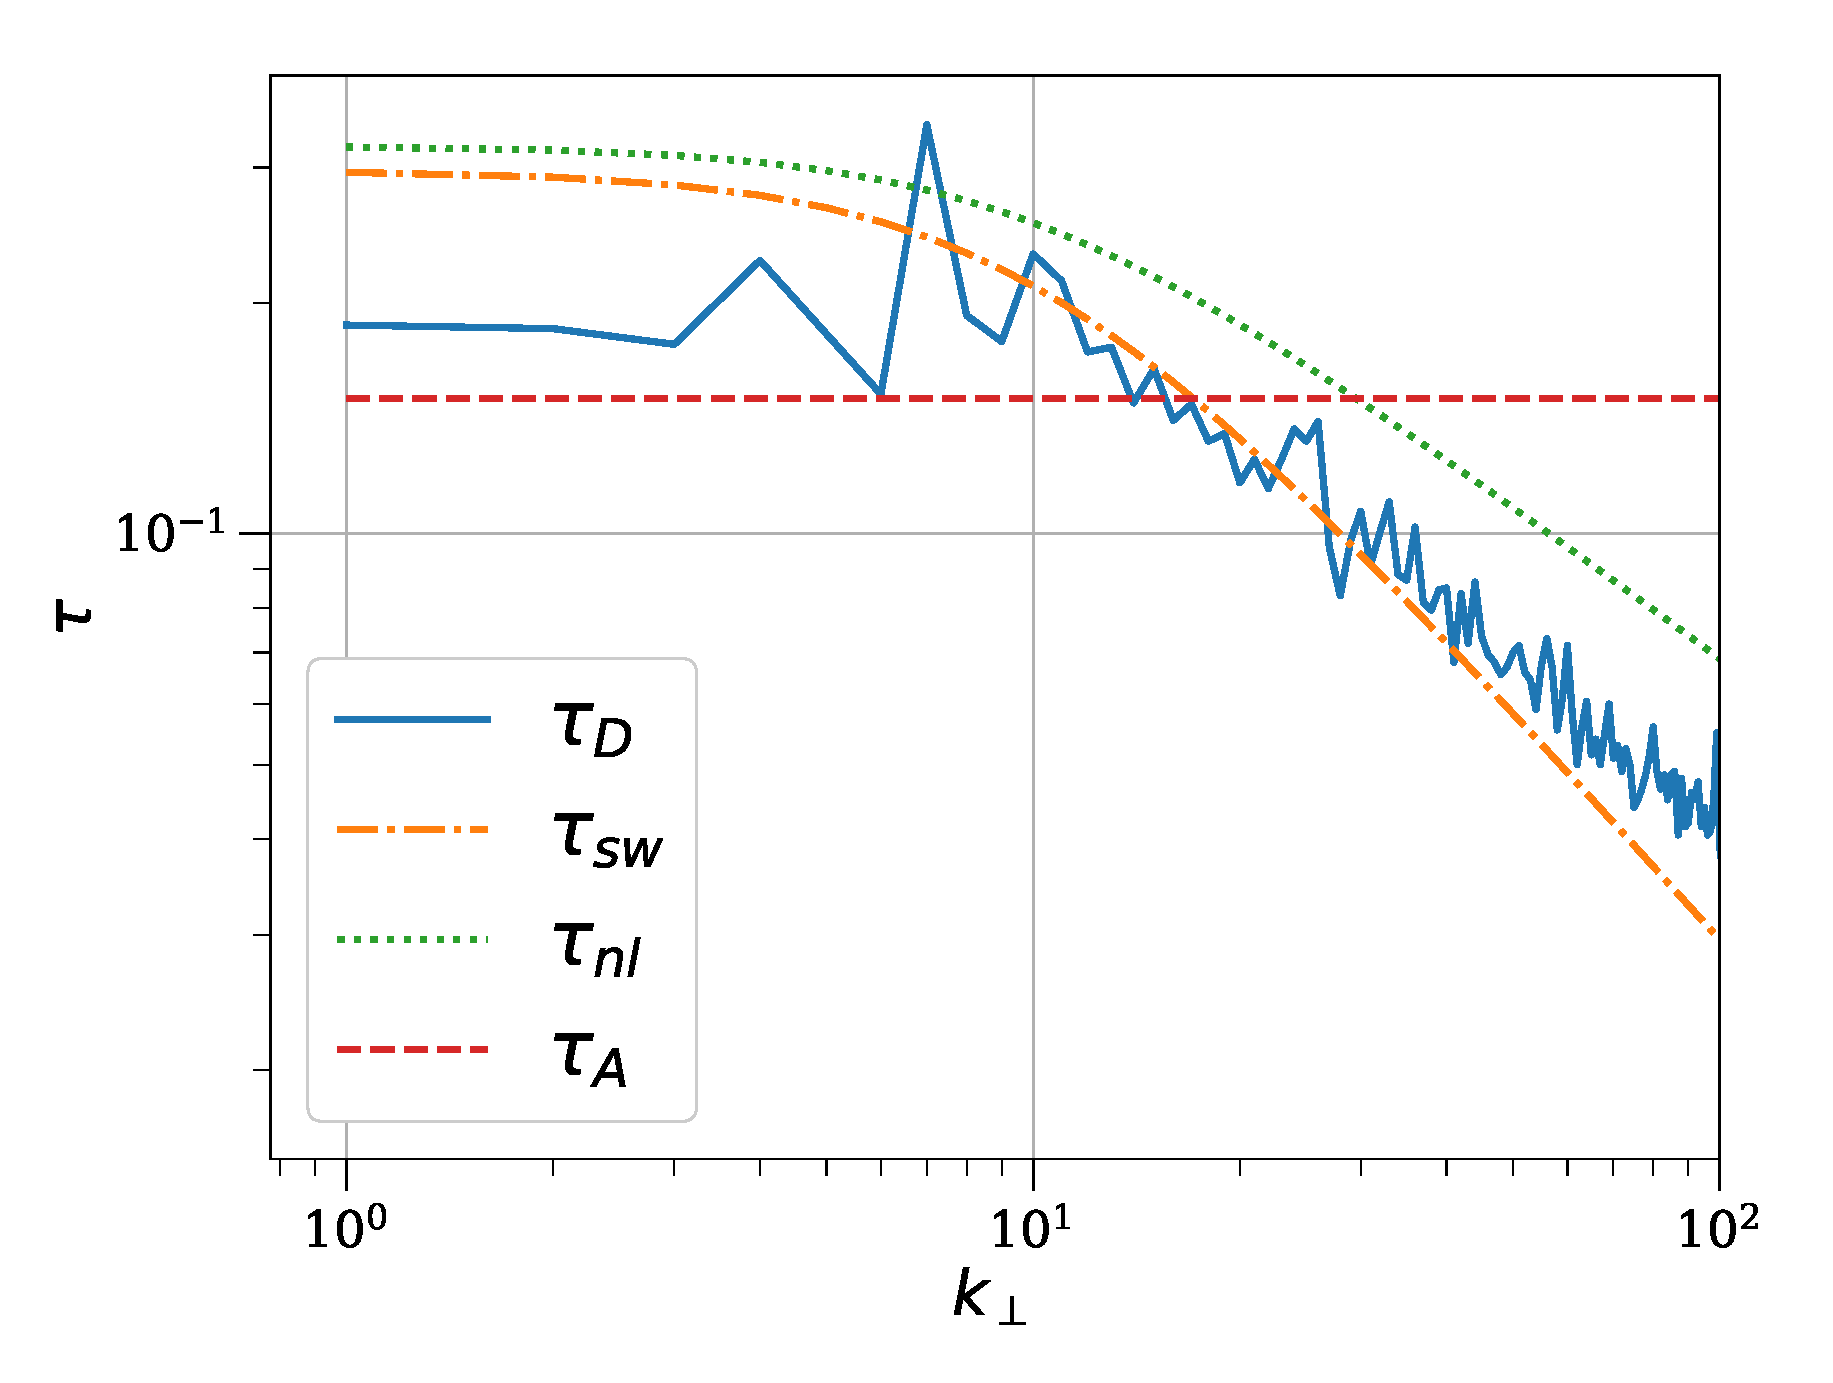
\includegraphics[width=0.95\columnwidth]{CrossHelicity/fig5_B1_Hc03_zmz_kpara_10.eps}}
  \subfigure[$\vec{z}^+$, $B_0=1$, $\sigma_c=0.3$, $k_\parallel=10$]{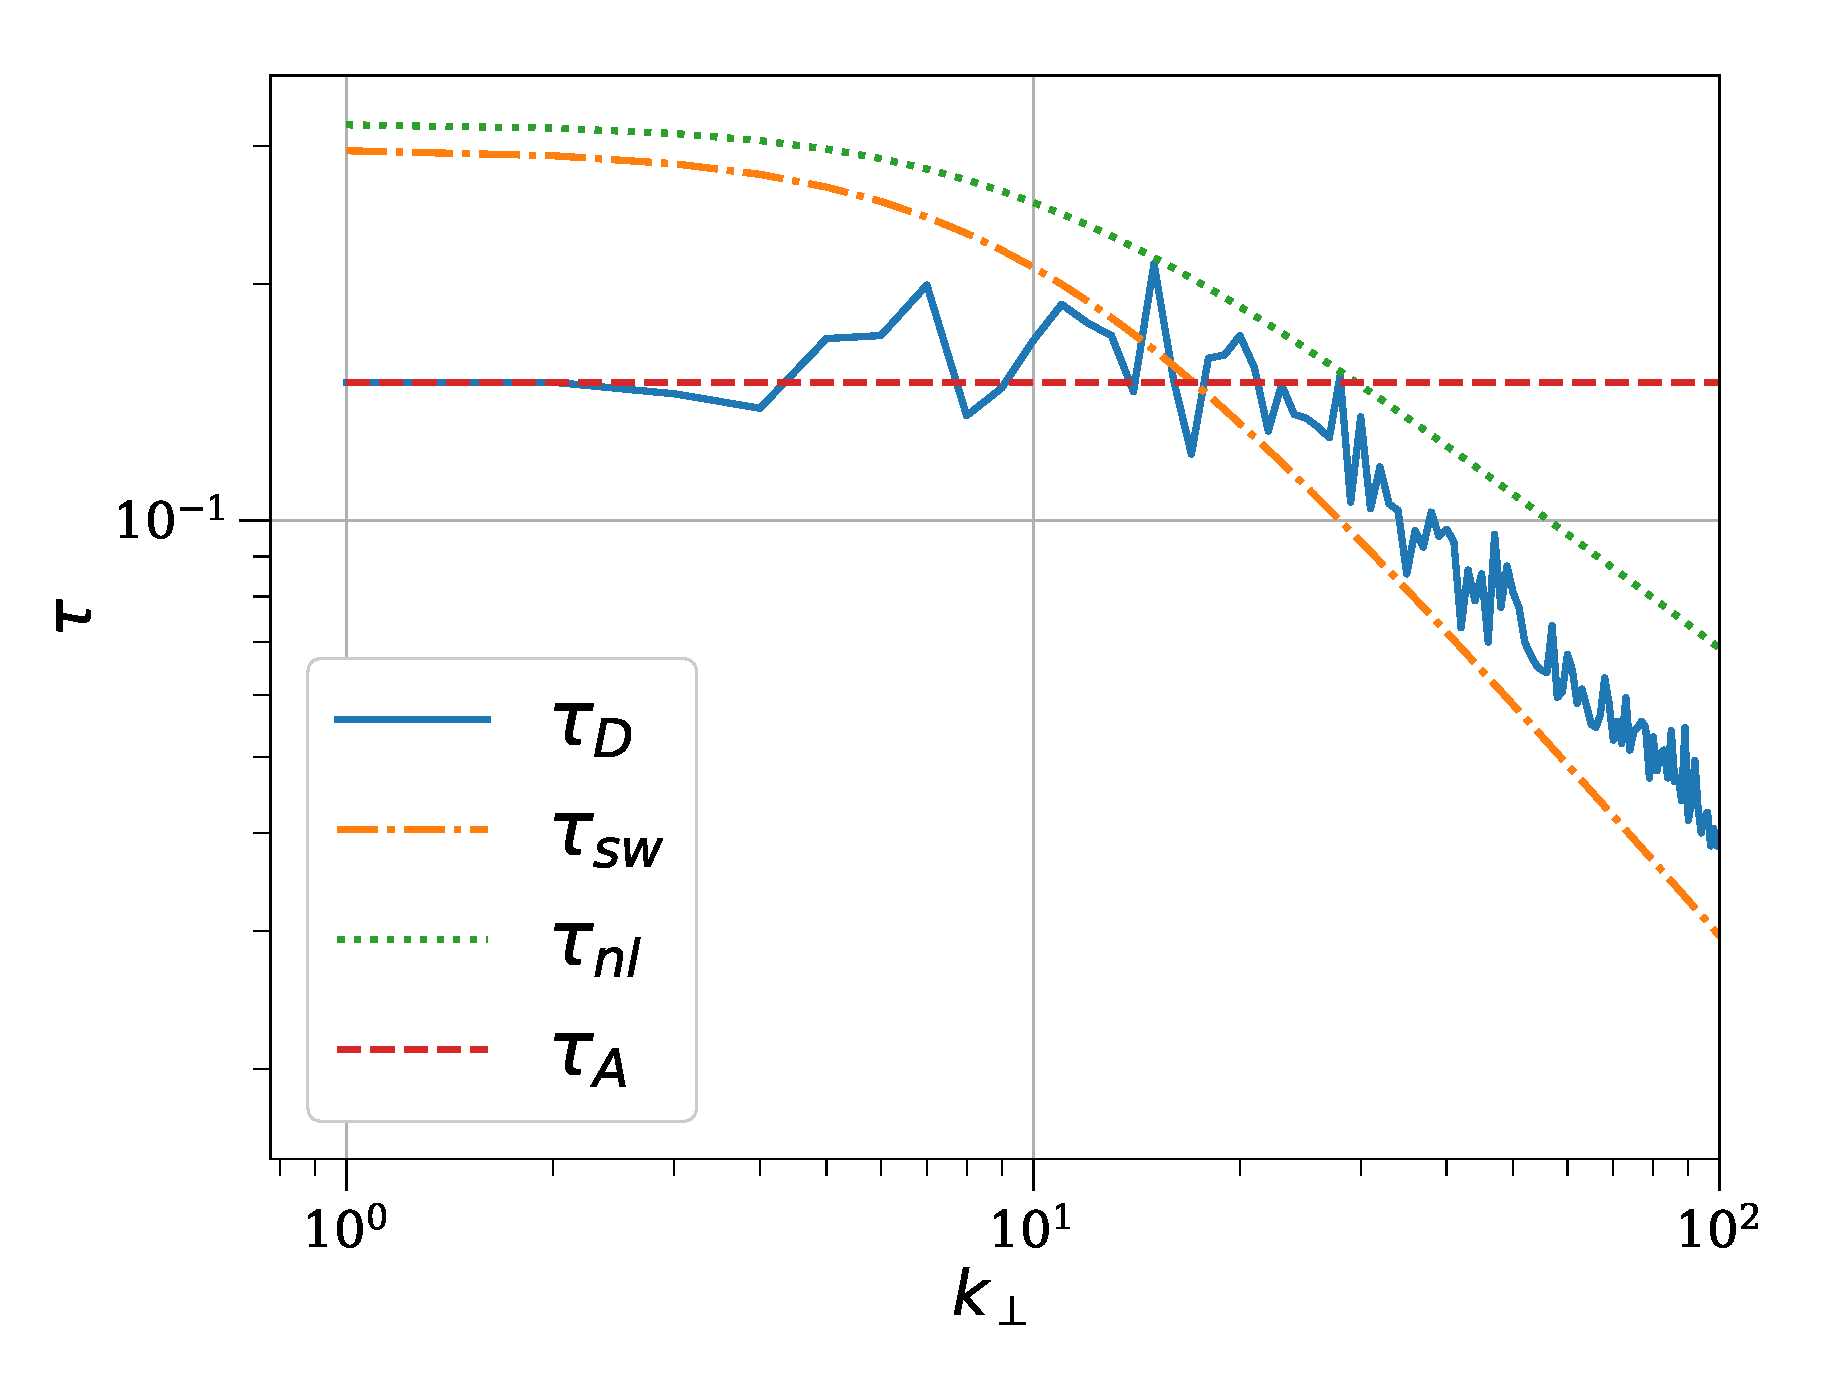
\includegraphics[width=0.95\columnwidth]{CrossHelicity/fig5_B1_Hc03_zpz_kpara_10.eps}}
  \caption{Decorrelation times $\tau_D$ for the run with $B_0=1$ and $\sigma_c=0.3$, for $k_\parallel=10$ constant and as a function of $k_\perp$. Panel (a) corresponds to $\vec{z}^-$ and panel (b) to $\vec{z}^+$. The theoretical prediction for the sweeping time $\tau_{sw}$, the non-linear time $\tau_{nl}$, and the Alfv\'en time $\tau_A$ are indicated as references.}
  \label{fig5:z+_vs_z-}
\end{figure}

Notar que para los casos con $B_0 \neq 0$, la energía no está
distribuida isotrópicamente en los espectros axisimétricos en la
\cref{fig2:isocontourns}. La energía tiende a acumularse en modos con
valores pequeños de $k_\parallel$ a medida que se incrementa $B_0$, y
para $B_0=4$ y $8$, una fracción sustancial de la energía se acumula
en las vecindades de las curvas que satisfacen
$\tau_A \approx \tau_{sw}$ y $\tau_A \approx \tau_{nl}$.


\subsection{Wavenumber-frequency spectra}\label{sec:wk}

Los principales resultados del presente estudio se encuentra resumidos
en las \cref{fig3:B0_spectrum_Hc, fig3:B025_spectrum_Hc,
  fig3:B1_spectrum_Hc, fig3:B8_spectrum_Hc}, que cuantifican el
comportamiento espacio-temporal de los campos de Els\"asser
separadamente. Estas figuras muestran el espectro normalizado en
función de los vectores de onda y la frecuencia, para las variables
$\vec{z}^+$ y $\vec{z}^-$, para simulaciones con diferentes valores
del campo medio de fondo $B_0$ y helicidad cruzada normalizada
$\sigma_c$. Como los espectros son multidimensionales, en todos los
casos mostamos fetas del espectro con $k_\perp=0$ y en función de
$k_\parallel$ y $\omega$.

La \cref{fig3:B0_spectrum_Hc} muestra estos espectros
espacio-temporales para las simulaciones con $B_0=0$. En este caso, la
relación de dispersión para las fluctuaciones Alfvénicas pasa a ser
$\omega=0$, y las ondas de Alfvén resultan indistinguibles (en este
espectro) de los modos lentos tales como los \textit{eddies}
turbulentos. La relación de \sweeping, para \textit{eddies} con
velocidad $v_{rms}$, se convierte en $\omega=\pm v_{rms} k$, y en la
práctica, como todos los \textit{eddies} turbulentos con esta
velocidad (o más baja) pueden barrer aleatoriamente estructuras de
pequeña escala en el flujo, la relación para \sweeping aleatorio pasa
a ser $|\omega| \leq v_{rms} k$. Ambas relaciones se indican
respectivamente con líneas rayada y sólida en la
\cref{fig3:B0_spectrum_Hc}.

La acumulación de la energía en los espectros de la
\cref{fig3:B0_spectrum_Hc} pueden verse para todos los modos en la
región encerrada por la relación de \sweeping, evidenciando la
presencia de turbulencia fuerte en todas las escalas, más que
turbulencia de ondas o propagación lineal de ondas. Para valores
grandes de la helicidad cruzada normalizada ($\sigma_c = 0.9$), la
energía se acumula en modos con $\omega\approx 0$, y se observa más
energía en los modos de $\vec{z}^+$ que en $\vec{z}^-$. De estos
espectros, podemos concluir que para $B_0=0$ y $\sigma_c=0$, la escala
de tiempo dominante es la del \sweeping, mientras que para grandes
valores de $\sigma_c$, se vuelven dominantes o bien la escala temporal
no lineal o el tiempo de Alfvén.

La \cref{fig3:B025_spectrum_Hc} muestra los espectros
espacio-temporales para las simulaciones con $B_0=0.25$. En caso con
$\sigma_c=0$ muestra nuevamente un rango amplio de fluctuaciones en el
rango de frecuencias encerrado por la relación de \sweeping. A medida
que el valor de $\sigma_c$ aumenta, las fluctuaciones de $\vec{z}^+$
se vuelven dominantes, una situación más evitente aún en el caso con
$\sigma_c=0.9$. Ademaś, a medida que $\sigma_c$ se incrementa, la
energía en las fluctuaciones de $\vec{z}^+$ dejan el embudo definido
por la relación de \sweeping, y se concentran en la vecindad de la
relación de dispersión de las ondas de Alfvén $\omega^+ =
+\vec{V}_\textrm{A} \cdot \vec{k}$ (ver el caso con $\sigma_c=0.9$ en
la \cref{fig3:B025_spectrum_Hc}). Notar que la elección de signos para
ondas descriptas por $\vec{z}^\pm={\vec z}_0^\pm e^{i(\vec{k} \cdot
  \vec{x}+\omega^\pm t)}$ sigue el hecho de que las transformadas de
Fourier utilizadas en espacio y en tiempo siguen la misma convención
de signos, y donde ${\vec z}_0^\pm$ son las amplitudes de las ondas.
De esta forma, el signo de $\omega^+$ implica que las fluctuaciones
$\vec{z}^+$ se propagan antiparalelamente al campo guía, como es
esperado. Sin embargo, en aparente contradicción, las ondas con
polarización opuesta, es decir, las fluctuaciones $\vec{z}^-$, también
pueblan la misma rama superior de la relación de dispersión de las
ondas de Alfvén, aunque con menos amplitud.

Como las fluctuaciones $\vec{z}^-$ satisfacen otra relación de
dispersión ($\omega^- = -\vec{V}_\textrm{A} \cdot \vec{k}$), en el
régimen lineal estas fluctuaciones deberían poblar, en cambio, la rama
inferior de la relación de dispersión mostrada en la
\cref{fig3:B025_spectrum_Hc}. Este comportamiento indica que las
fluctuaciones $\vec{z}^-$ también se propagan en el espacio real en la
dirección antiparalela al campo guía (es decir, con velocidad
negativa), en lugar de paralelamente a este campo (es decir, con
velocidad positiva), como cabría esperar. Dicho comportamiento fue
predicho por Hollweg \cite{hollweg_1990_wkb} para el viento solar y es
causado, por ejemplo, por reflexiones de ondas debido a fluctuaciones
de la densidad en el medio interplanetario, utilizando la expansión
WKB. En nuestro caso, el flujo es incompresible y la densidad es
uniforme en el espacio y constante en el tiempo.

\begin{figure*}
  \centering
  \subfigure[$\vec{z}^+$, $B_0=0.25$, $\sigma_c=0.3$, $k_\parallel=15$]{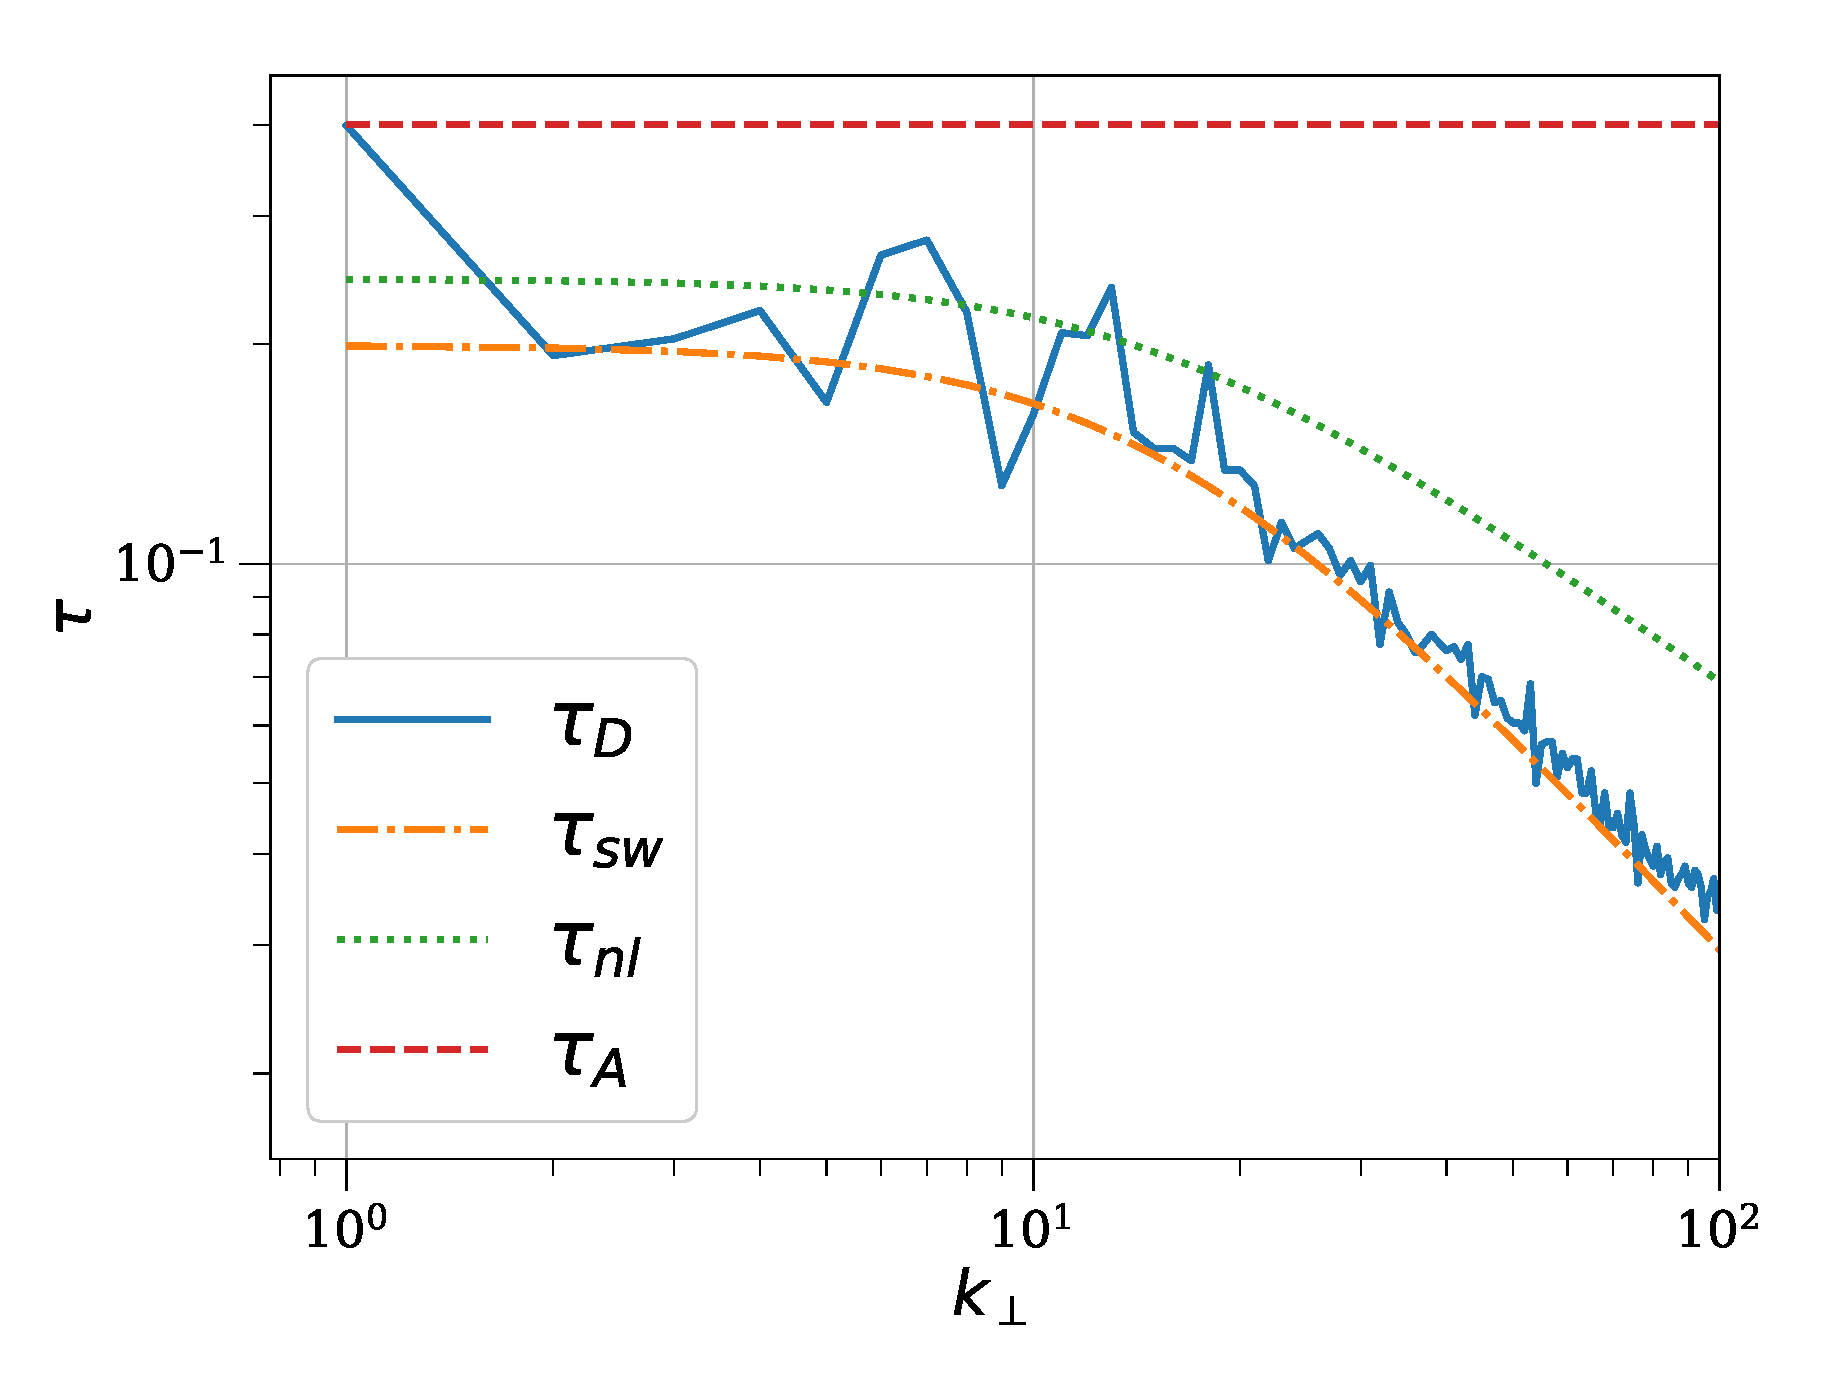
\includegraphics[width=0.9\columnwidth]{CrossHelicity/fig5_B025_Hc03_zpz_kpara_15.eps}}
  \subfigure[$\vec{z}^+$, $B_0=1$, $\sigma_c=0.3$, $k_\parallel=15$]{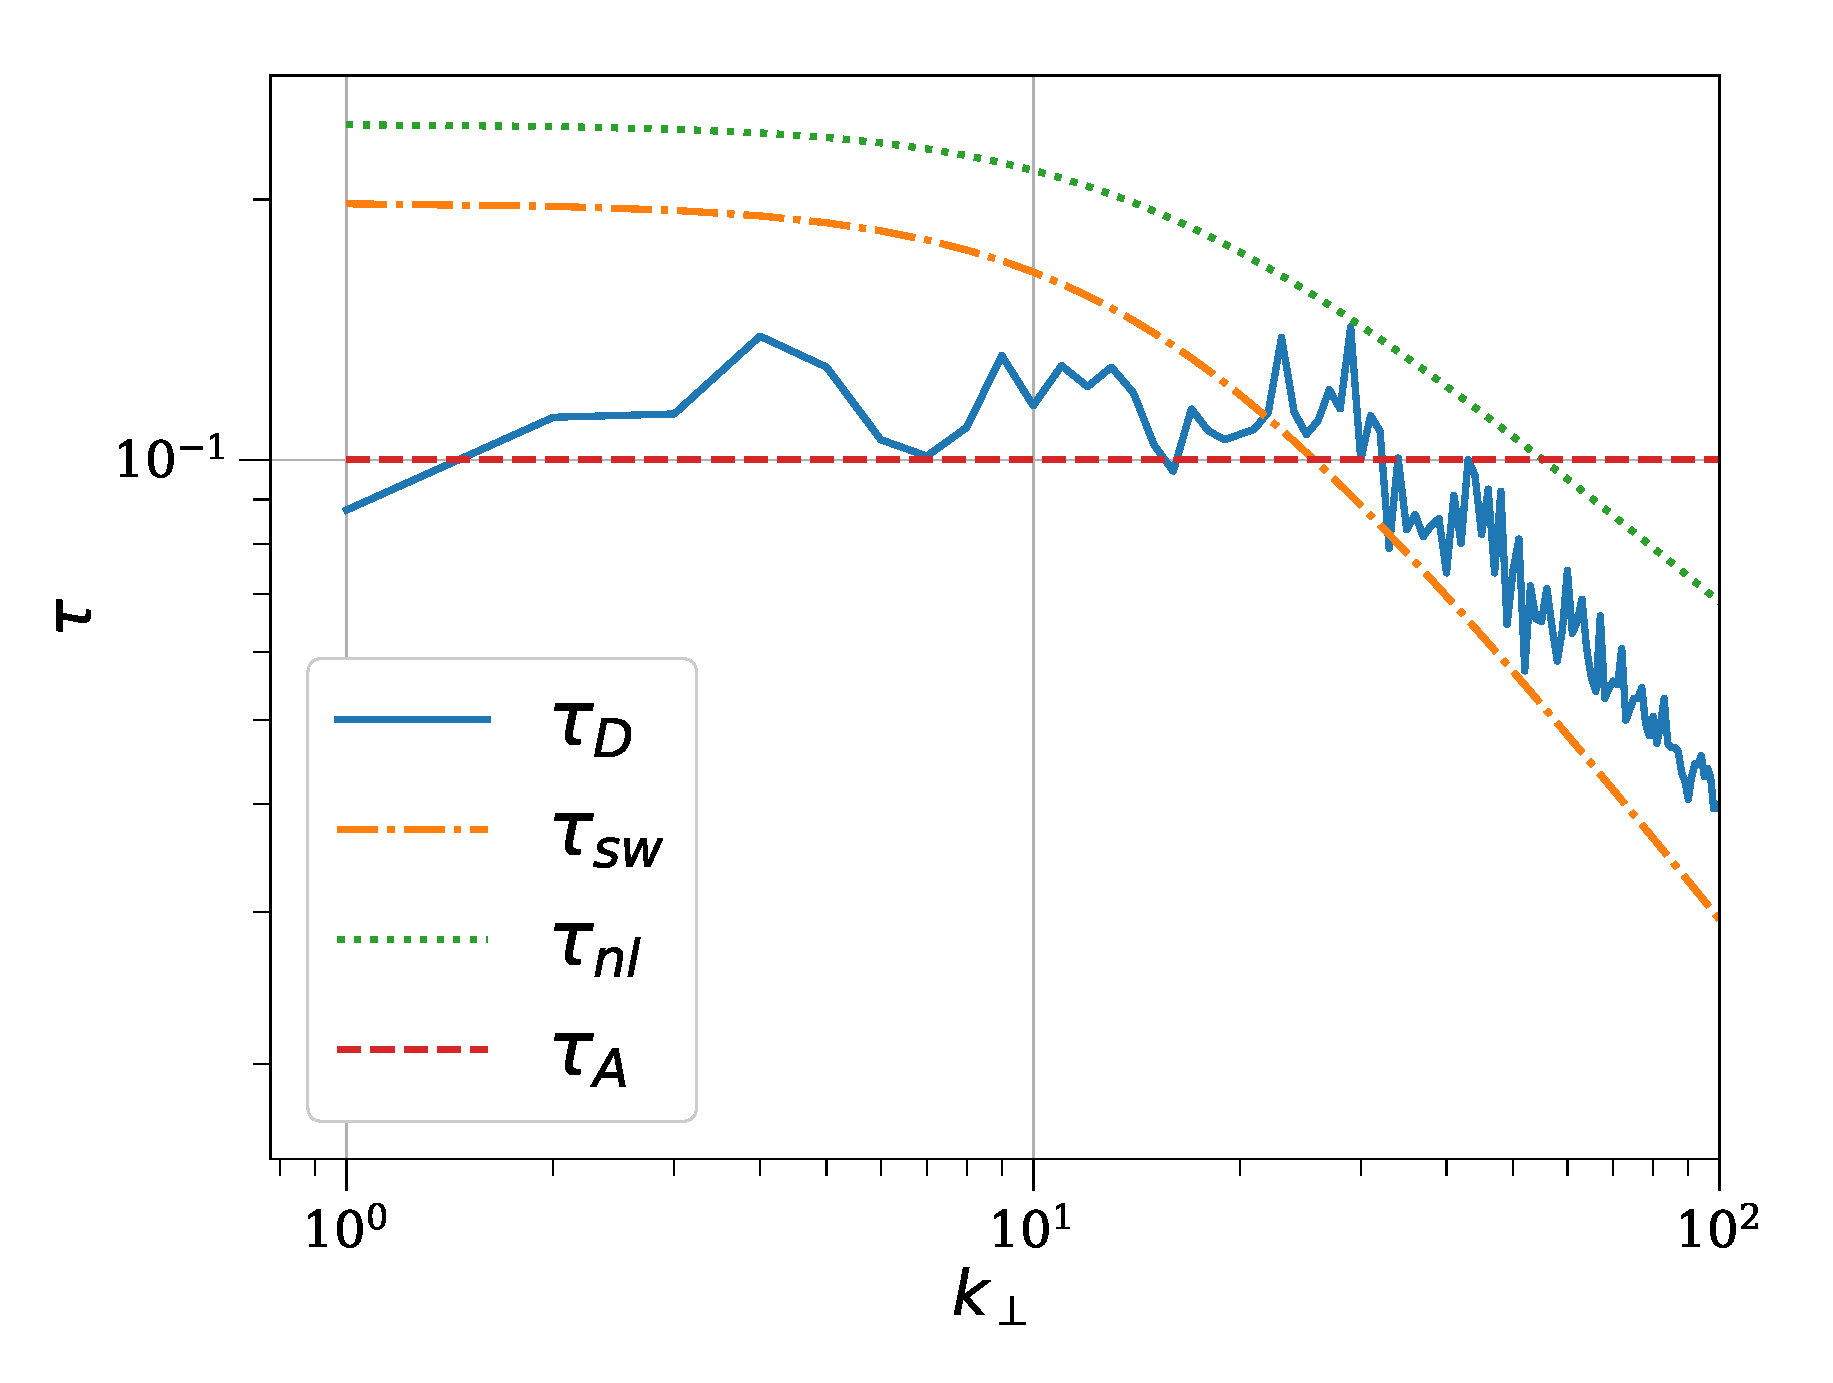
\includegraphics[width=0.9\columnwidth]{CrossHelicity/fig5_B1_Hc03_zpz_kpara_15.eps}}
  \subfigure[$\vec{z}^+$, $B_0=4$, $\sigma_c=0.3$, $k_\parallel=15$]{\includegraphics[width=0.9\columnwidth]{CrossHelicity/fig5_B4_Hc03_zpz_kpara_15.eps}}
  \subfigure[$\vec{z}^+$, $B_0=8$, $\sigma_c=0.3$, $k_\parallel=15$]{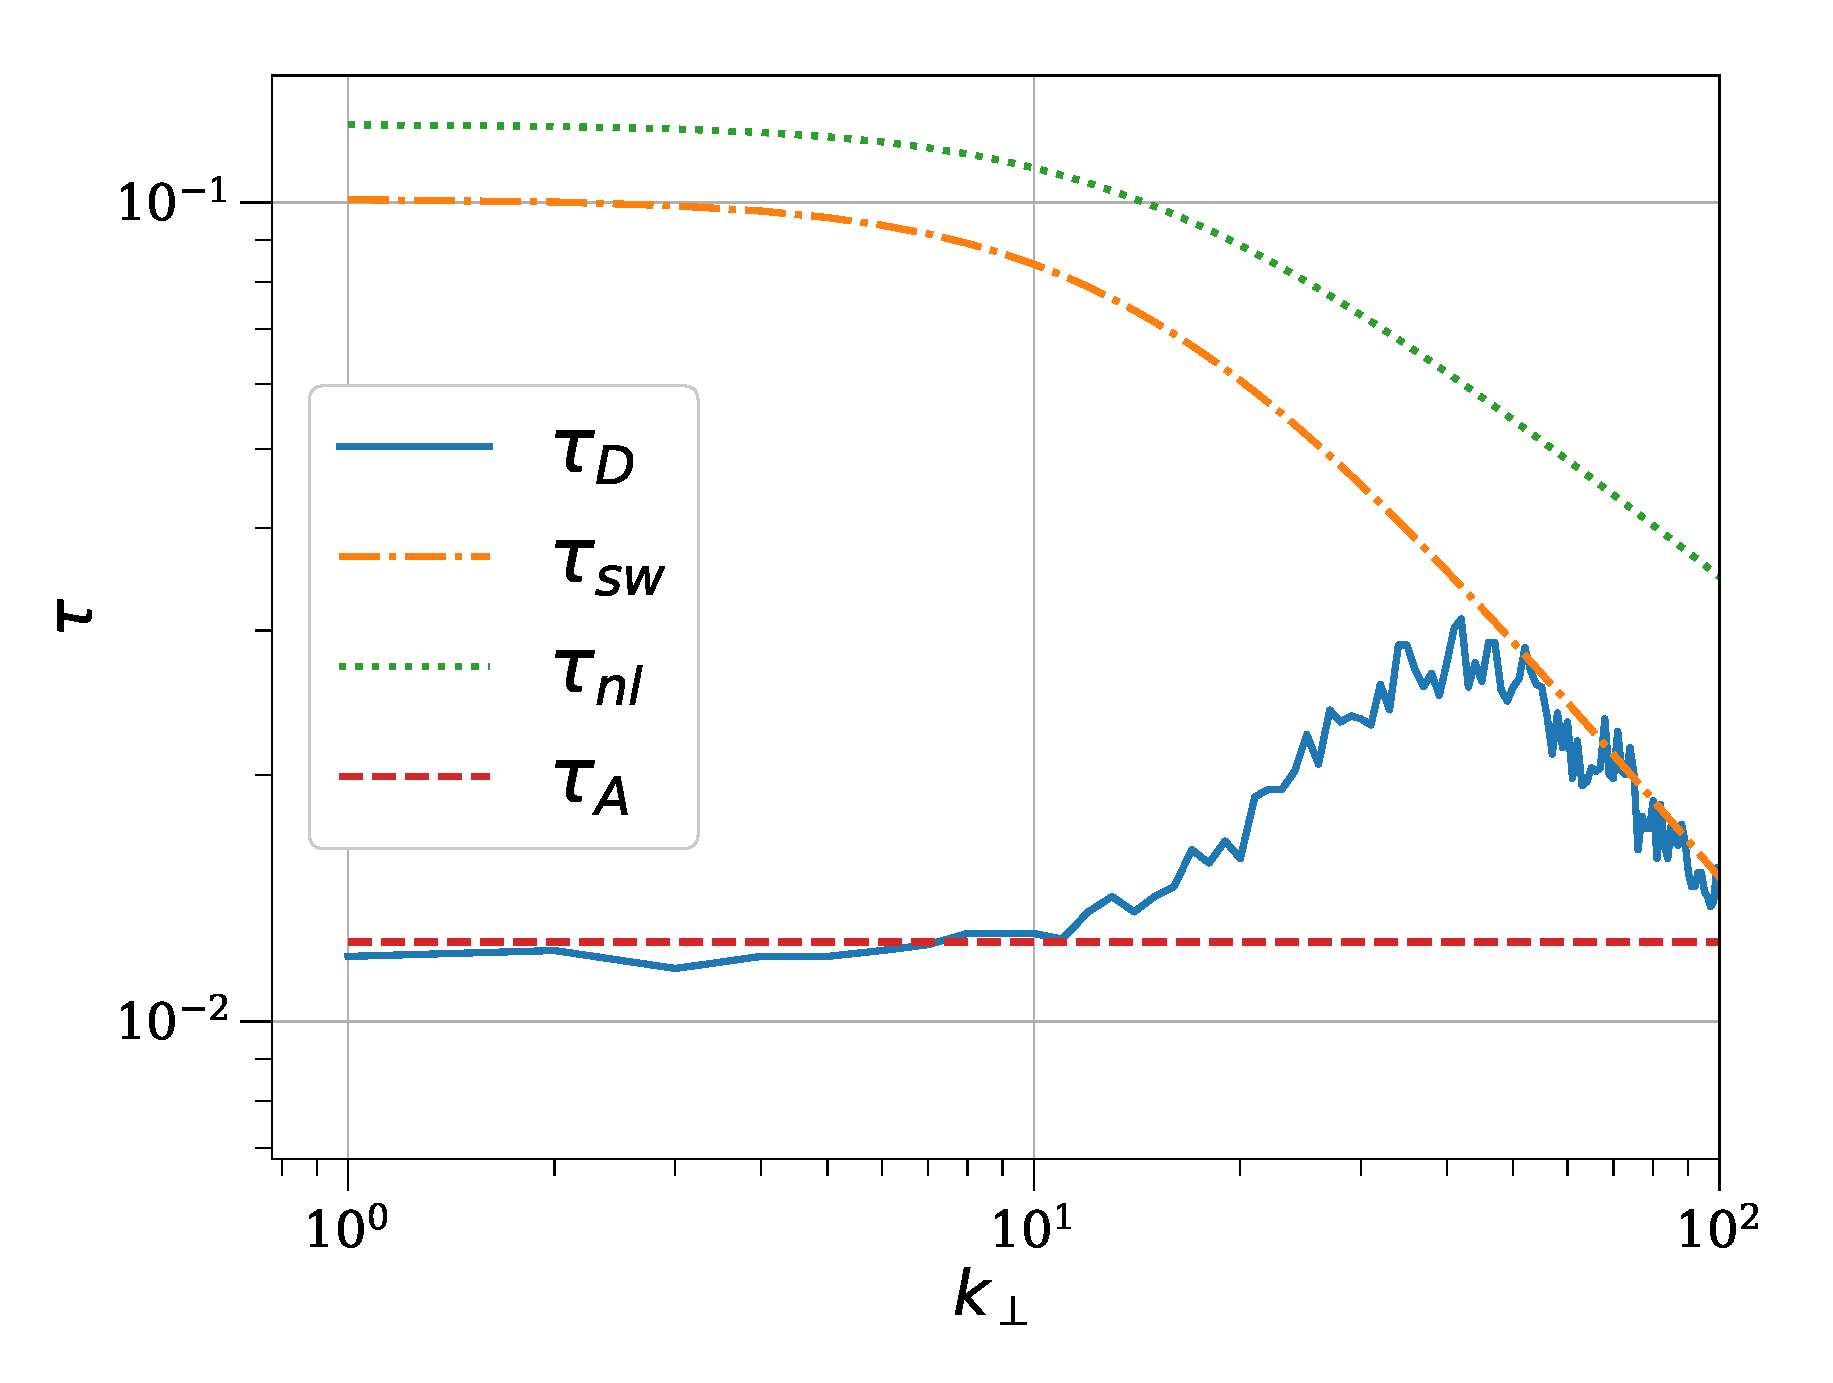
\includegraphics[width=0.9\columnwidth]{CrossHelicity/fig5_B8_Hc03_zpz_kpara_15.eps}}
    \caption{Decorrelation times $\tau_D$ for the $\vec{z}^+$ field in simulations with $\sigma_c = 0.3$ and (a) $B_0=0.25$, (b) $1$, (c) $4$, and (d) $8$, for $k_\parallel = 15$ and as a function of $k_\perp$. The theoretical prediction for the sweeping time $\tau_{sw}$, the non-linear time $\tau_{nl}$, and the Alfv\'en time $\tau_A$ are indicated as references.}
  \label{fig5:tD_vs_B0}
\end{figure*}

\begin{figure*}
  \centering
  \subfigure[$\vec{z}^+$, $B_0=0.25$, $\sigma_c=0.3$, $k_\perp=15$]{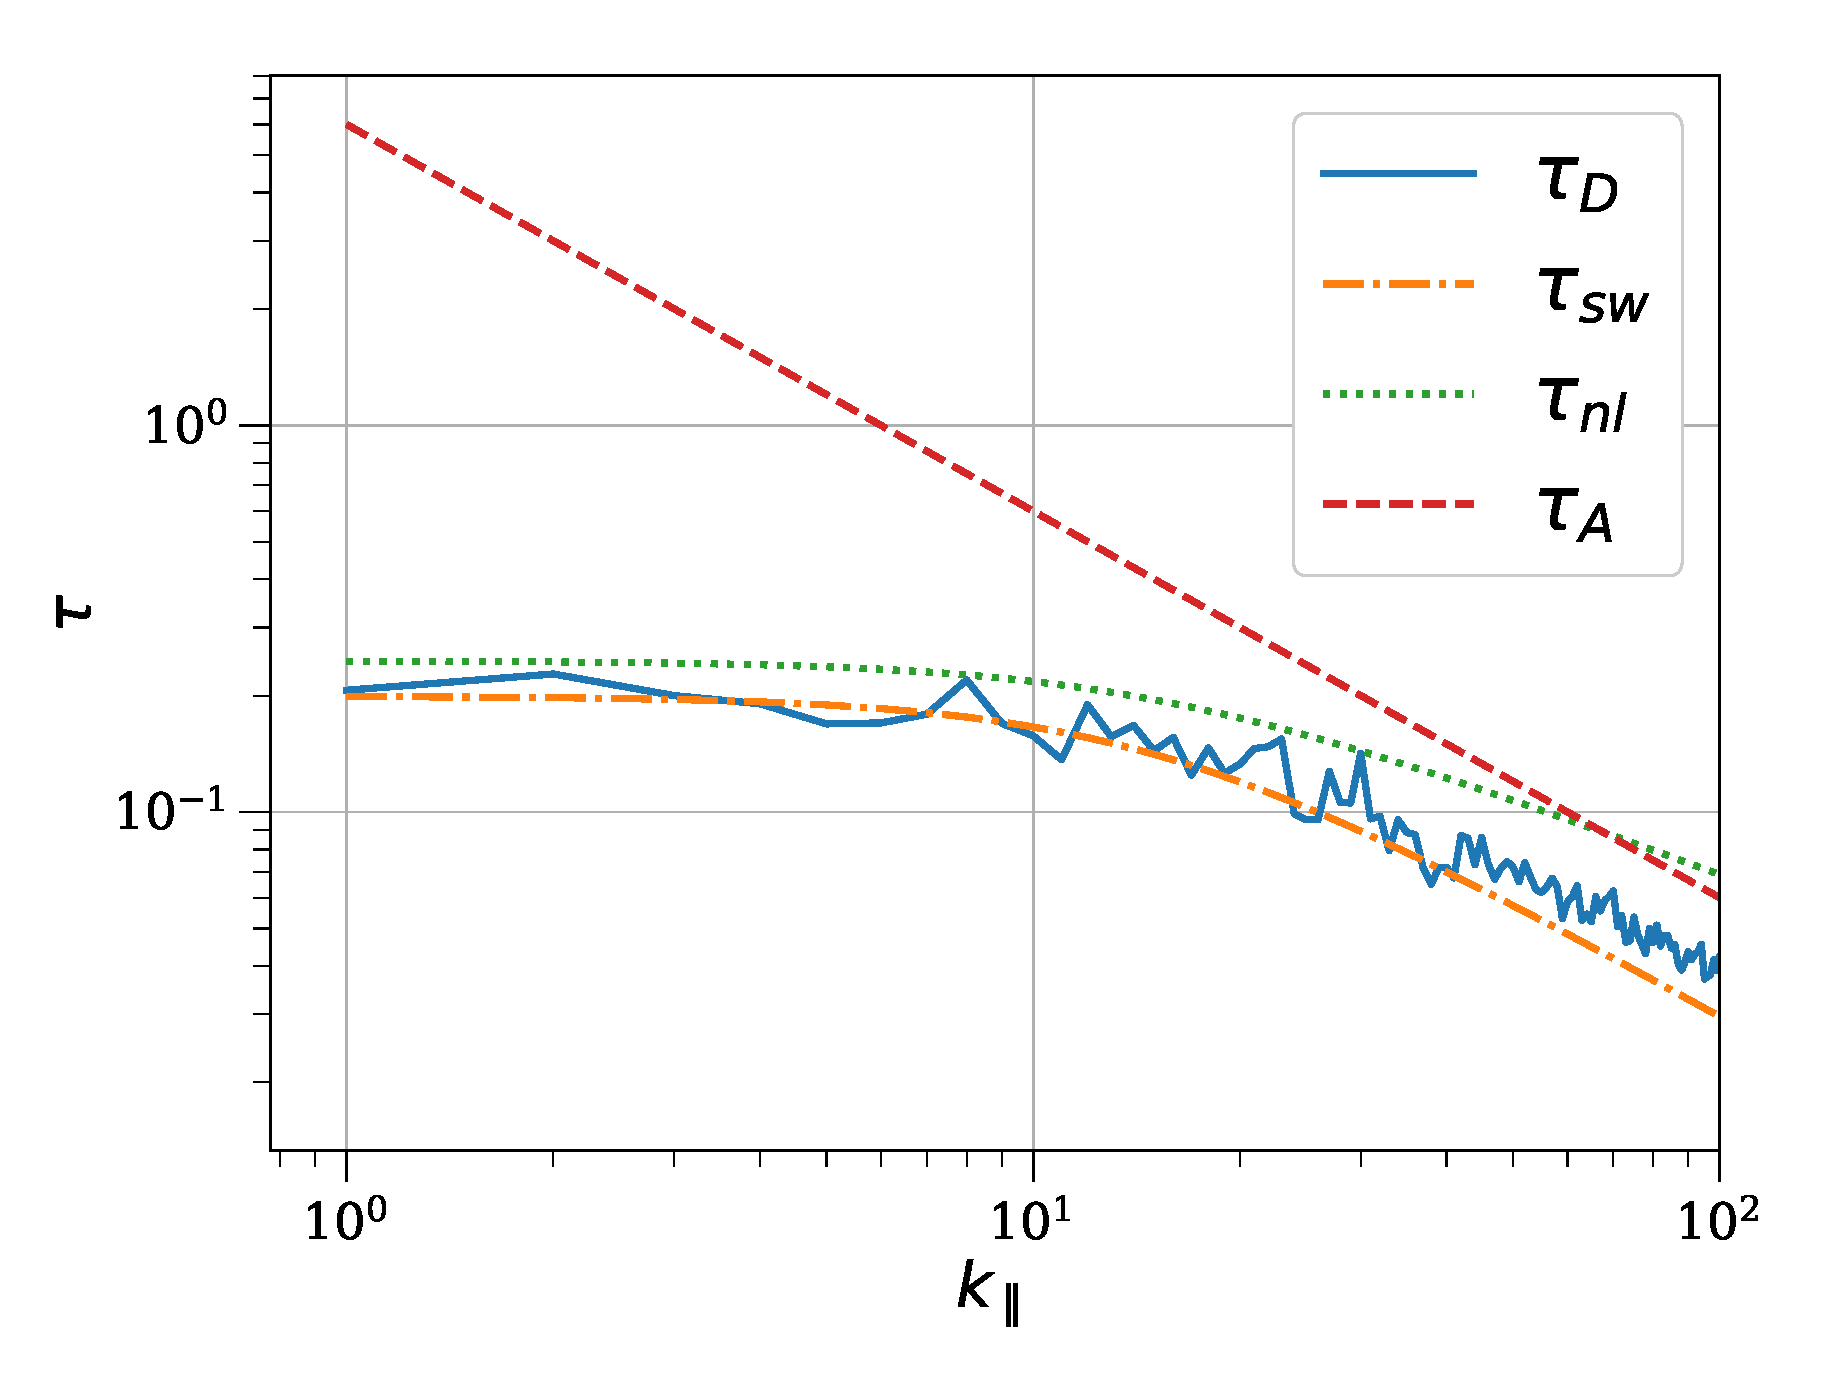
\includegraphics[width=0.9\columnwidth]{CrossHelicity/fig5_B025_Hc03_zpz_kperp_15.eps}}
  \subfigure[$\vec{z}^+$, $B_0=1$, $\sigma_c=0.3$, $k_\perp=15$]{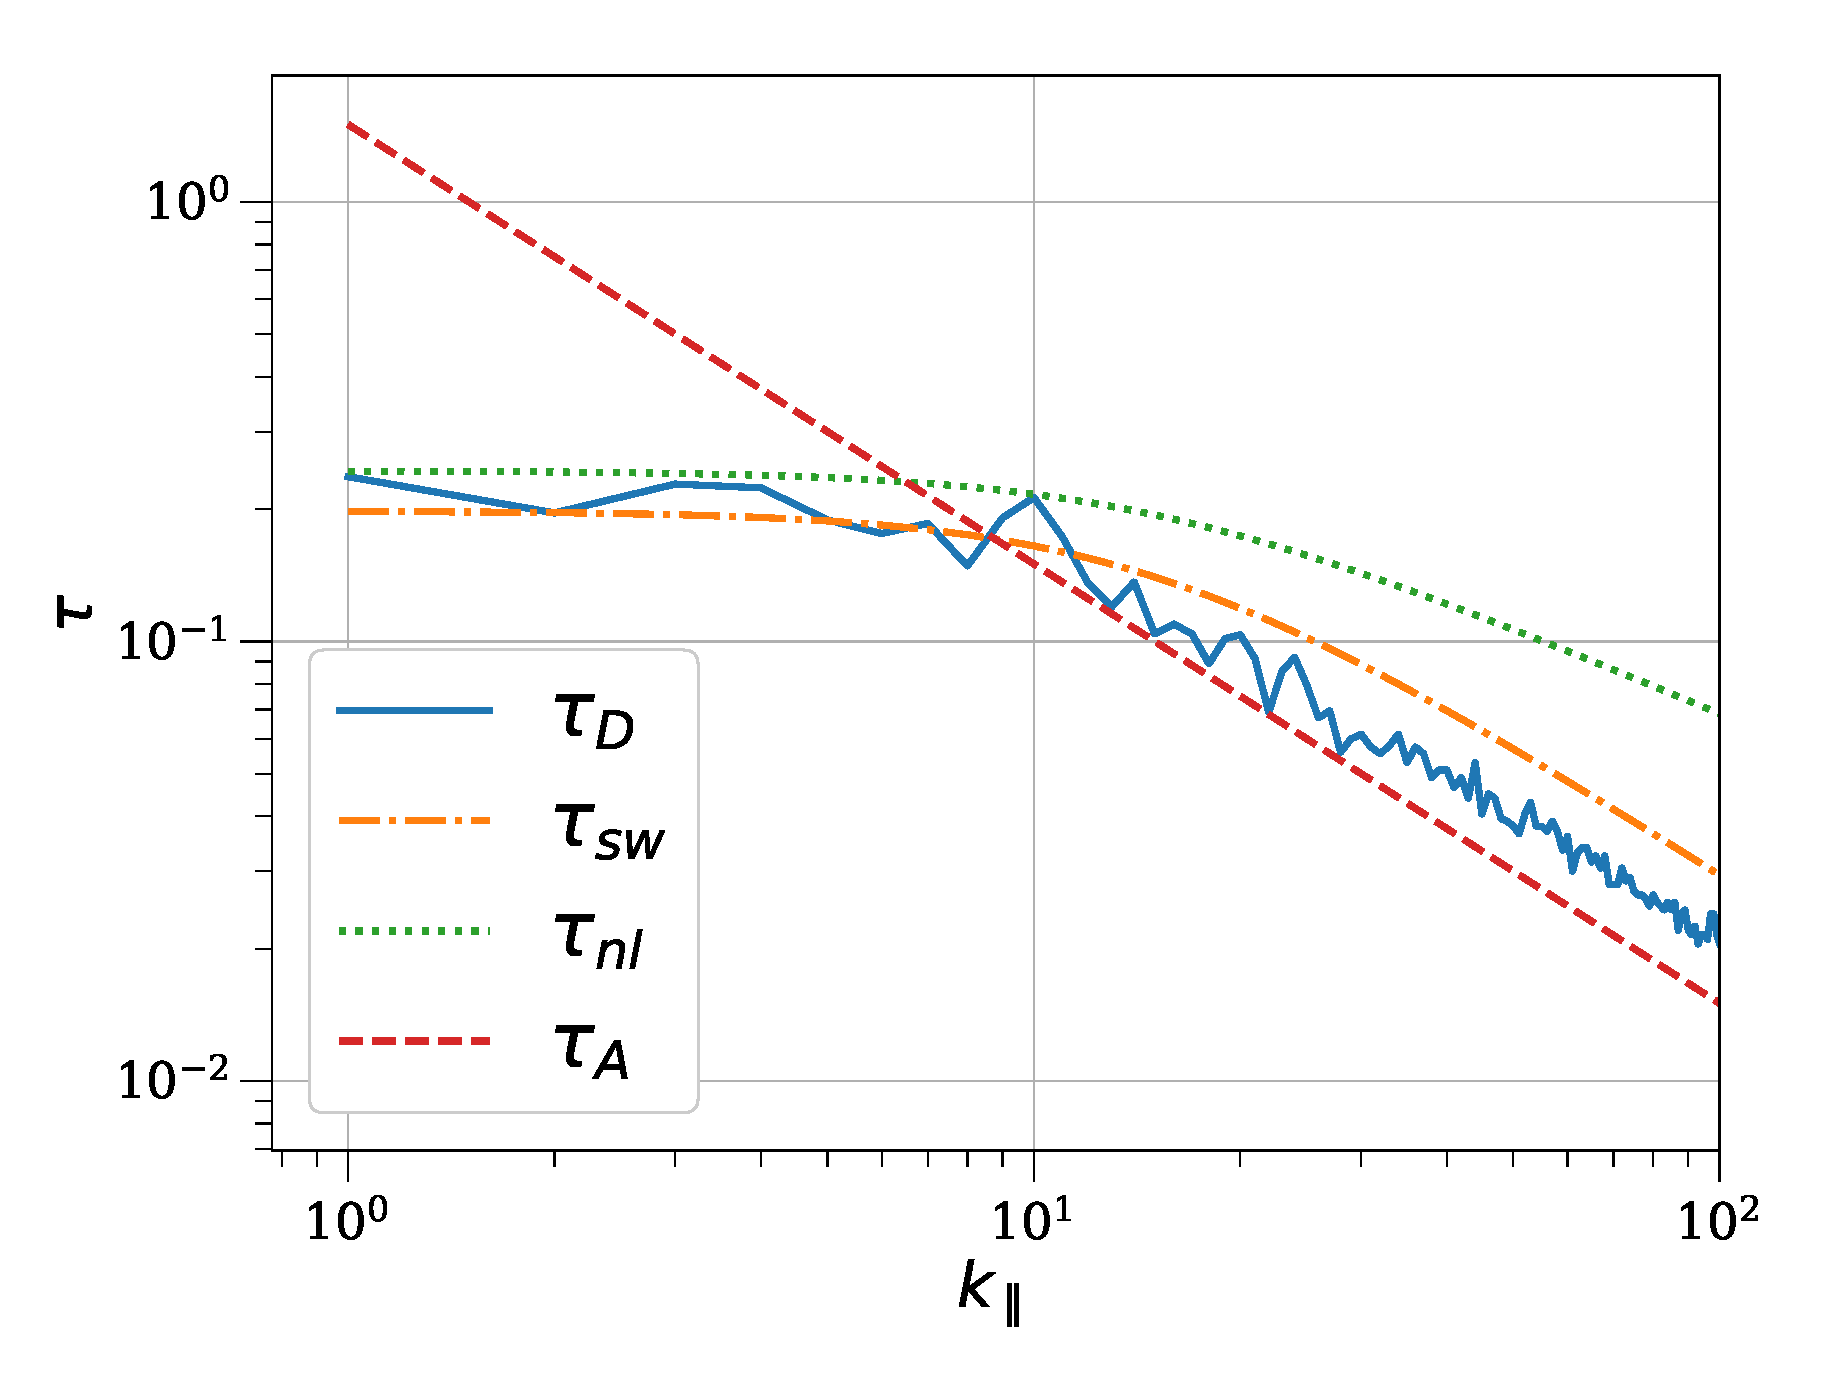
\includegraphics[width=0.9\columnwidth]{CrossHelicity/fig5_B1_Hc03_zpz_kperp_15.eps}}
  \subfigure[$\vec{z}^+$, $B_0=4$, $\sigma_c=0.3$, $k_\perp=15$]{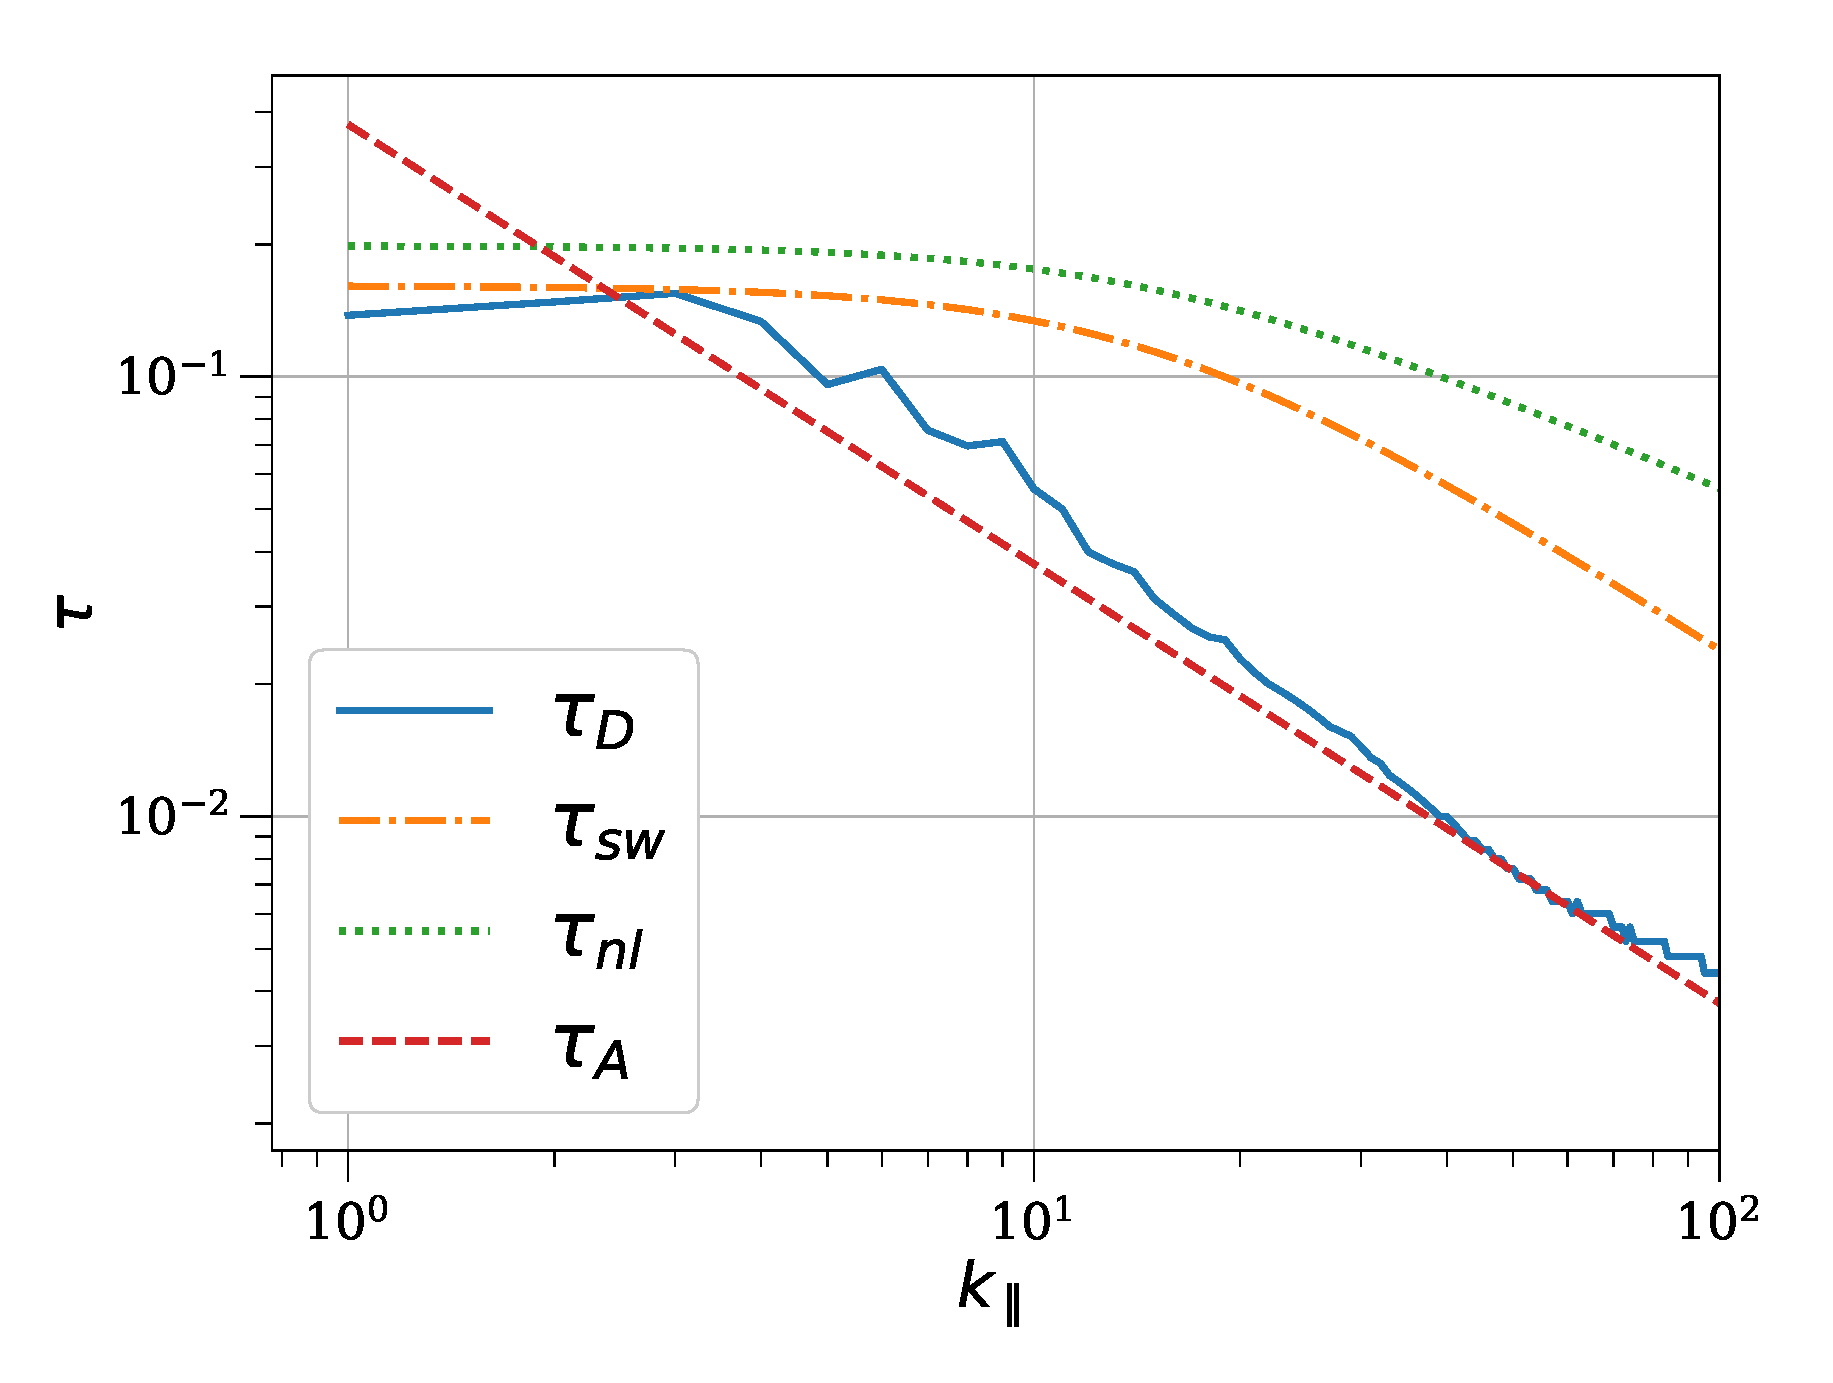
\includegraphics[width=0.9\columnwidth]{CrossHelicity/fig5_B4_Hc03_zpz_kperp_15.eps}}
  \subfigure[$\vec{z}^+$, $B_0=8$, $\sigma_c=0.3$, $k_\perp=15$]{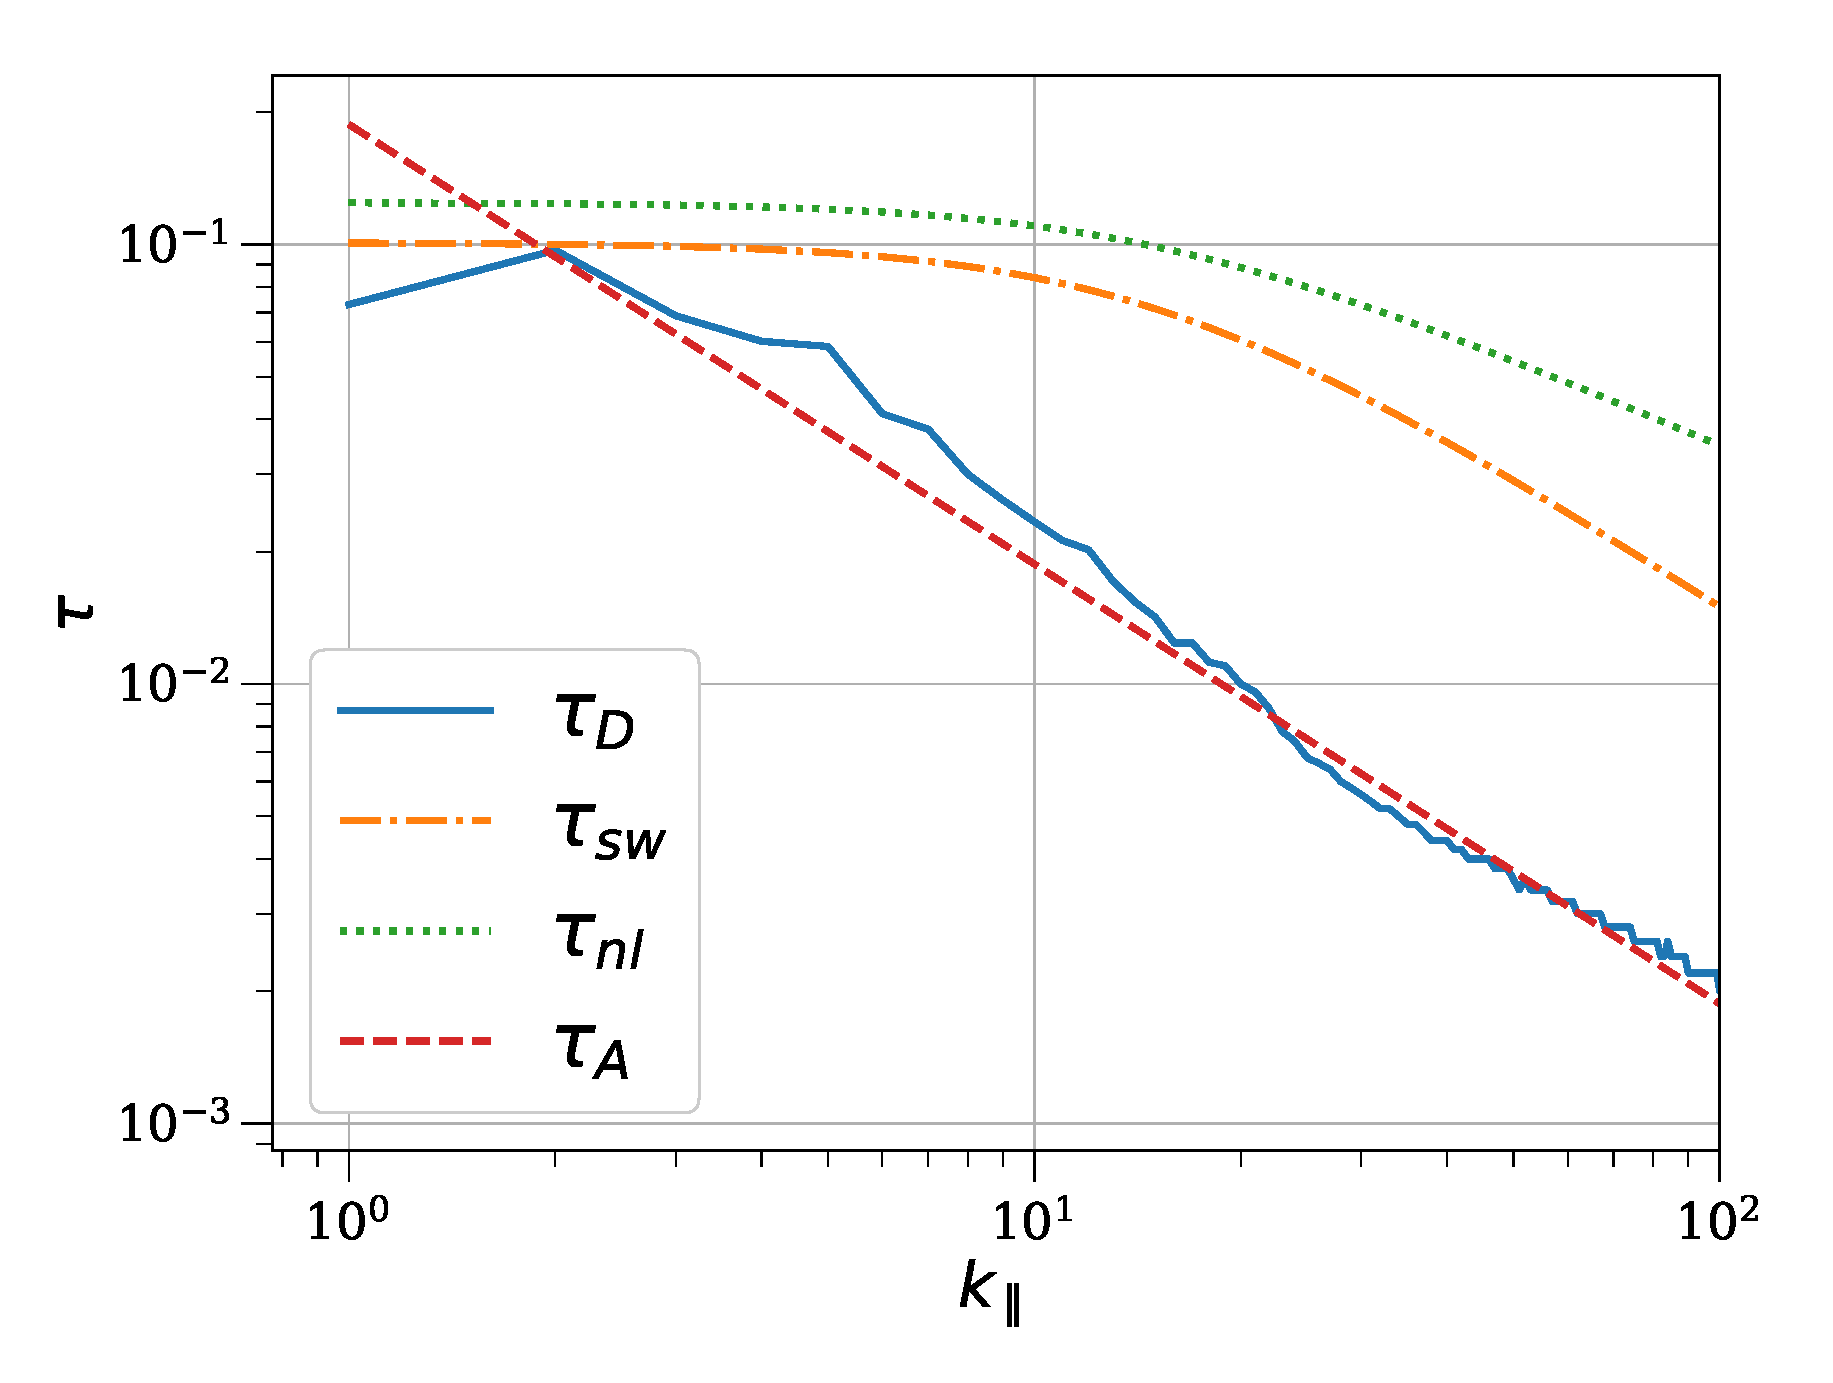
\includegraphics[width=0.9\columnwidth]{CrossHelicity/fig5_B8_Hc03_zpz_kperp_15.eps}}
    \caption{Decorrelation times $\tau_D$ for the $\vec{z}^+$ field in simulations with $\sigma_c = 0.3$ and (a) $B_0=0.25$, (b) $1$, (c) $4$, and (d) $8$, for $k_\perp=15$ and as a function of $k_\parallel$. The theoretical prediction for the sweeping time $\tau_{sw}$, the non-linear time $\tau_{nl}$, and the Alfv\'en time $\tau_A$ are indicated as references.}
  \label{fig5:tD_vs_B0_2}
\end{figure*}

\begin{figure}
  \centering
  \subfigure[$\sigma_c = 0$]{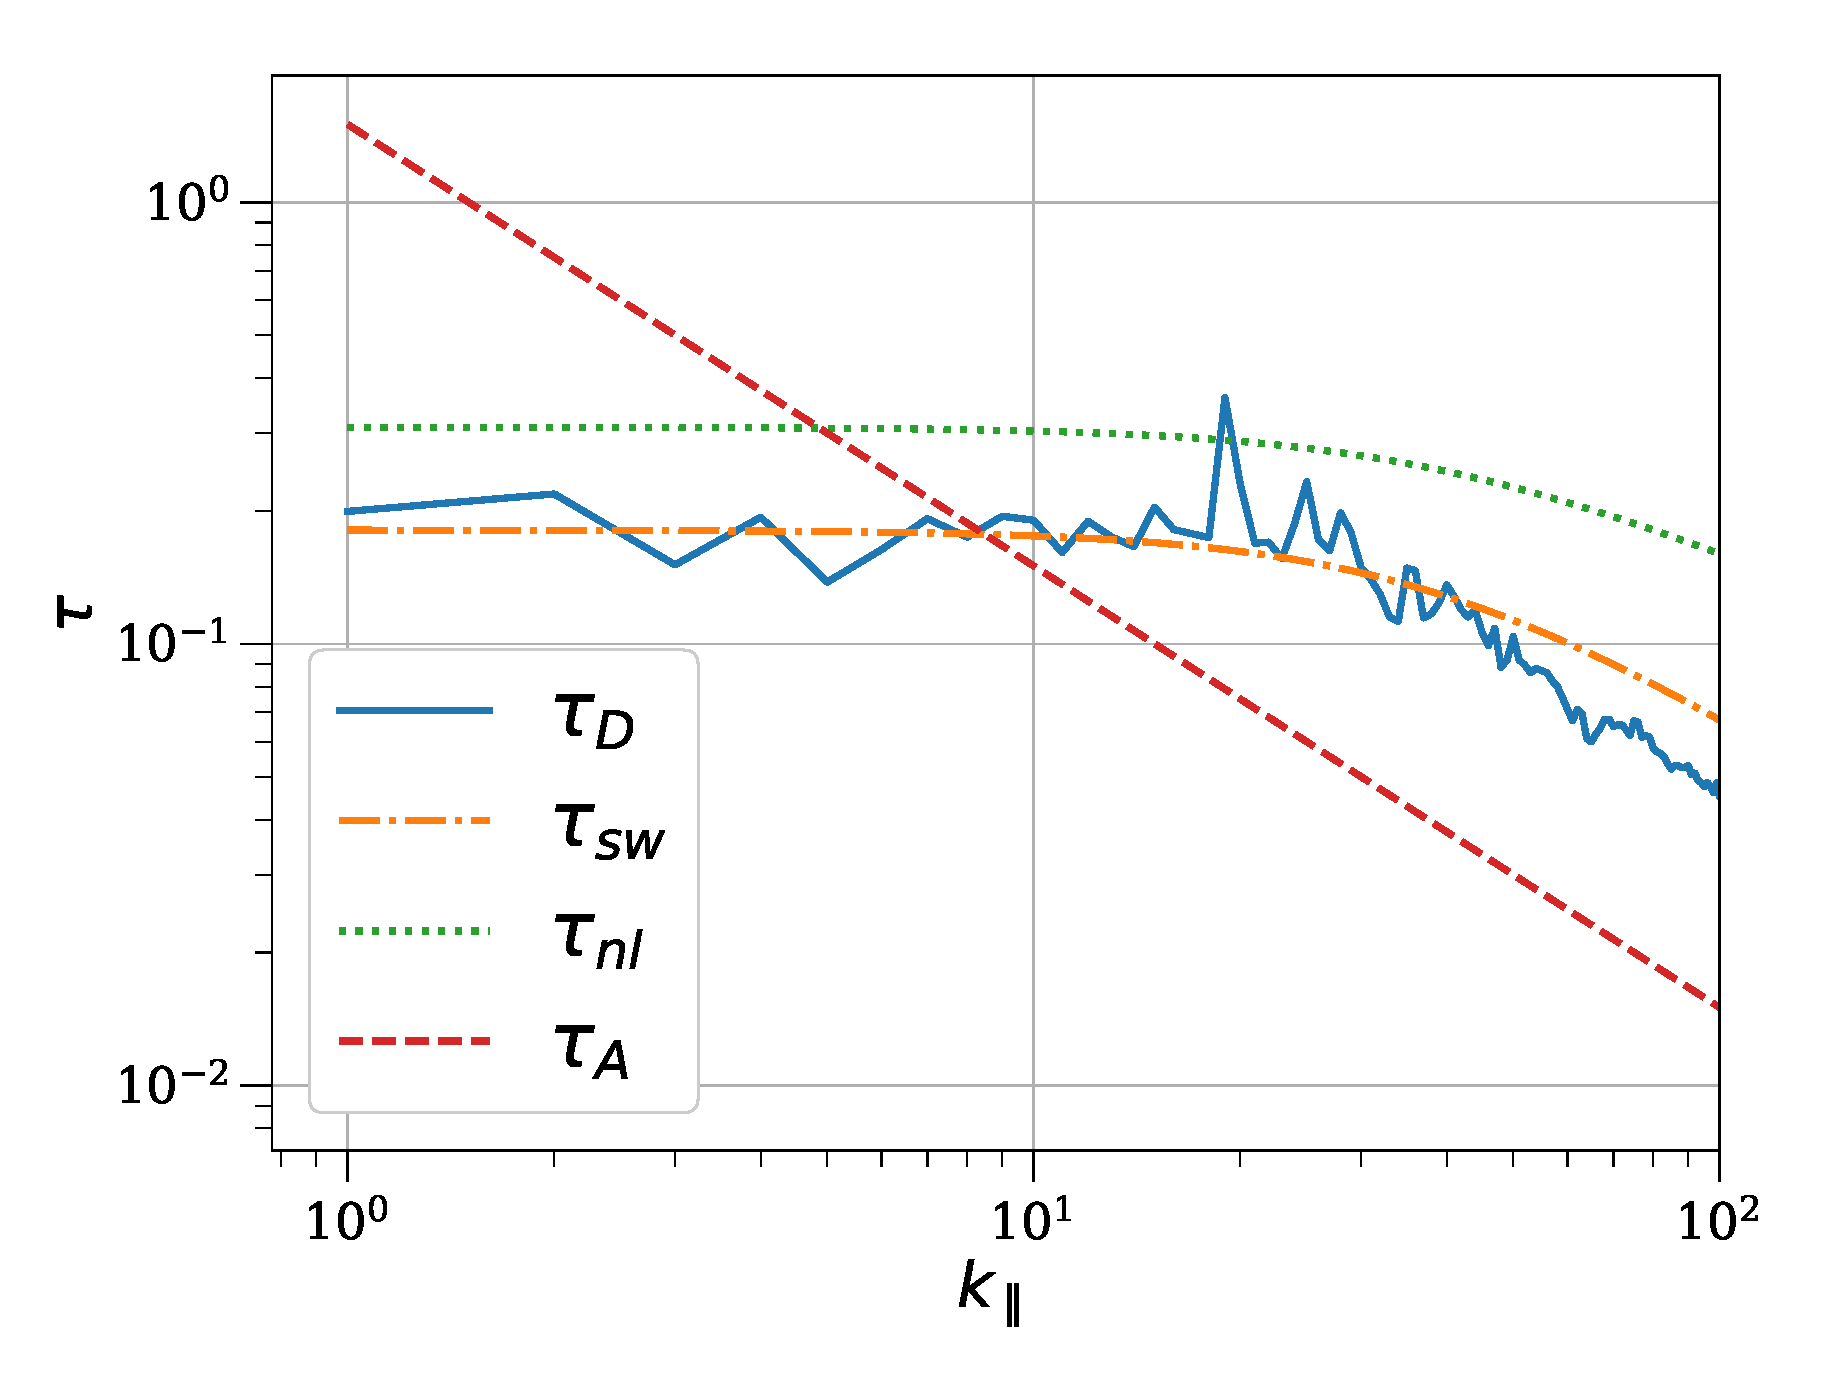
\includegraphics[width=0.95\columnwidth]{CrossHelicity/fig5_B1_Hc00_zpz_kperp_40.eps}}
  \subfigure[$\sigma_c = 0.3$]{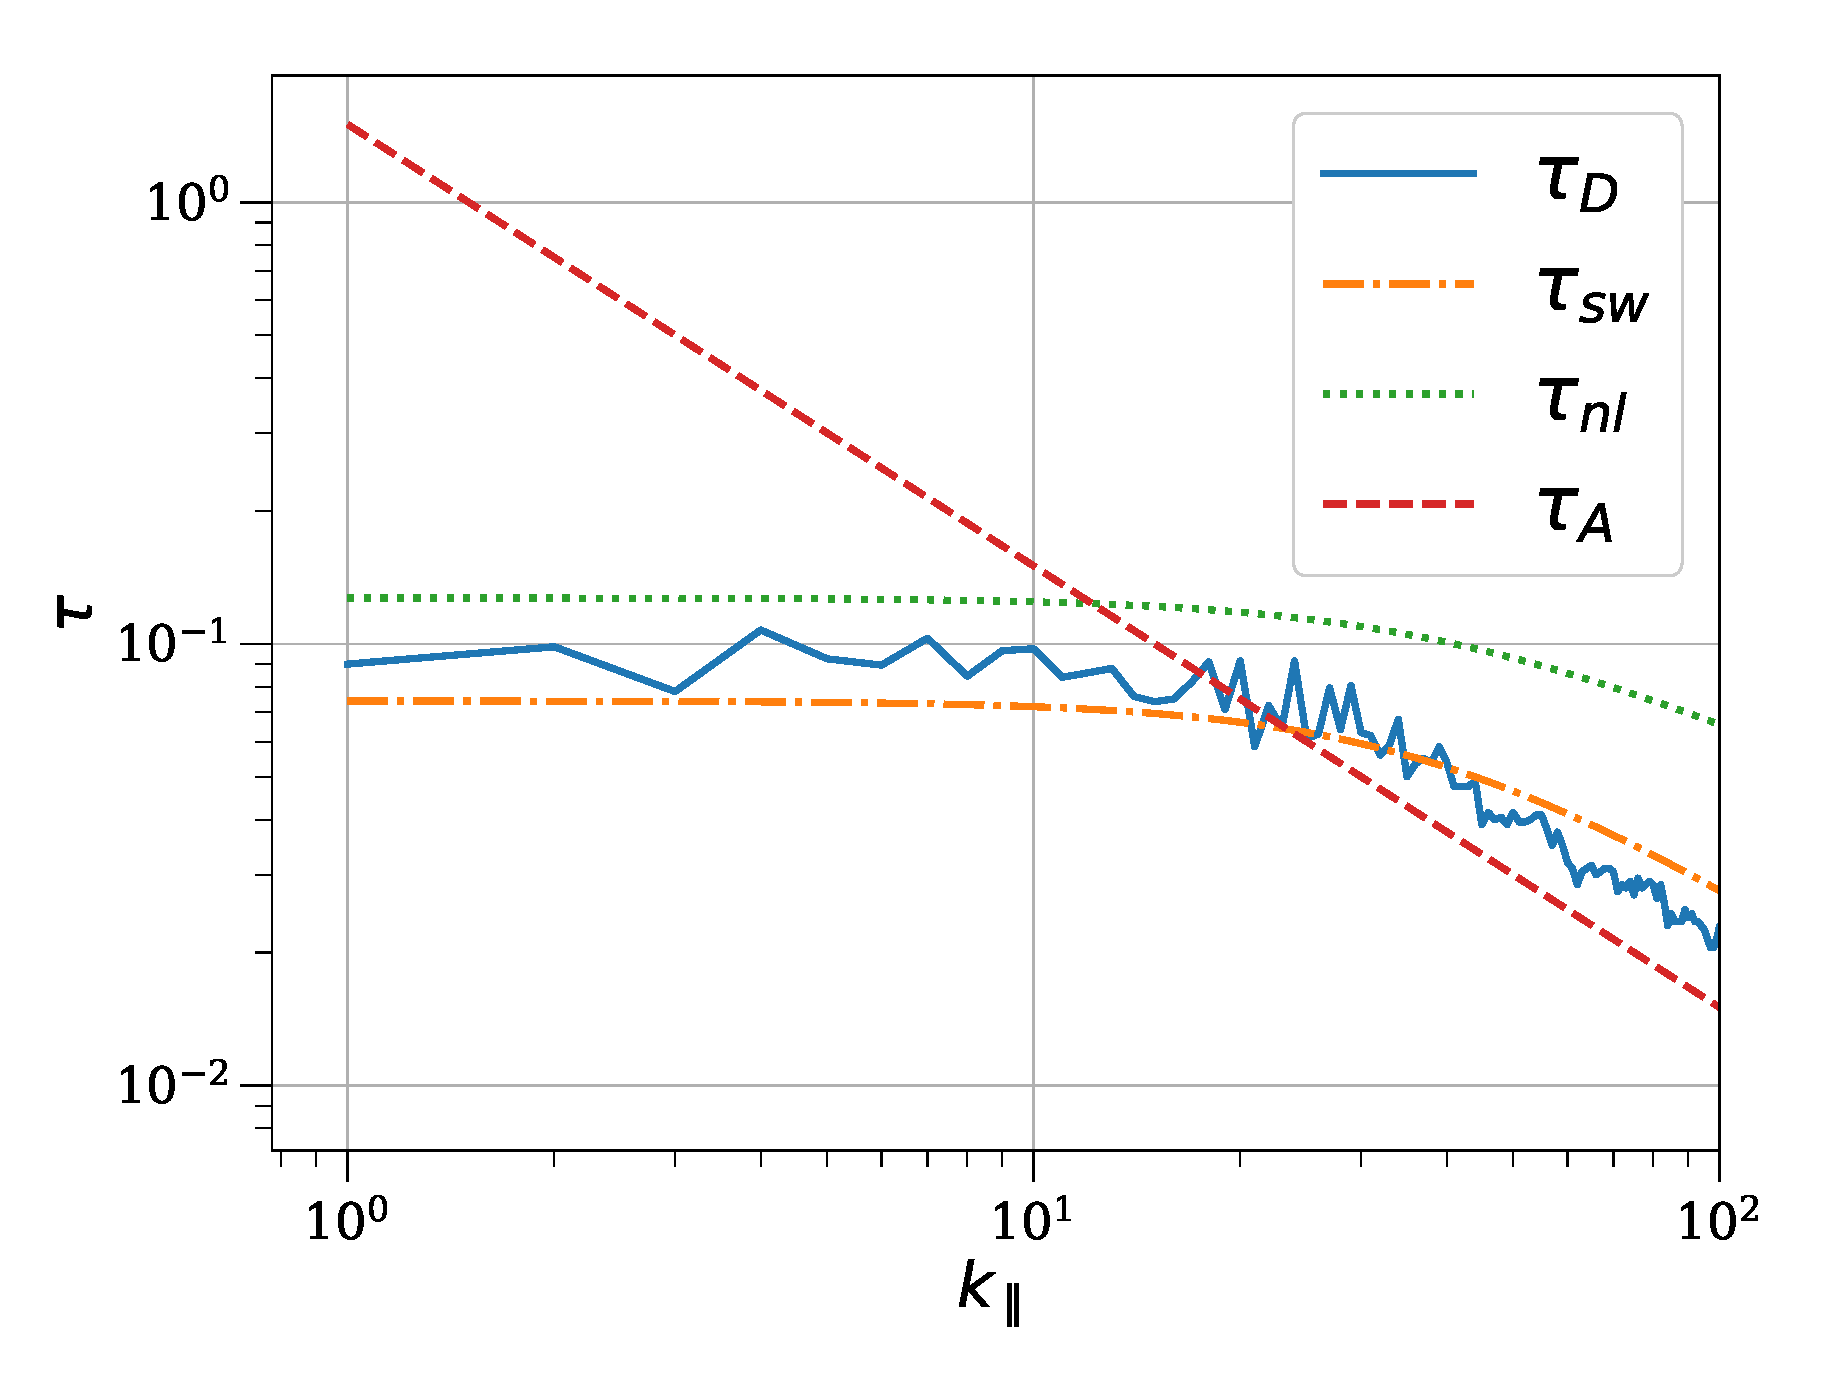
\includegraphics[width=0.95\columnwidth]{CrossHelicity/fig5_B1_Hc03_zpz_kperp_40.eps}}
  \subfigure[$\sigma_c = 0.9$]{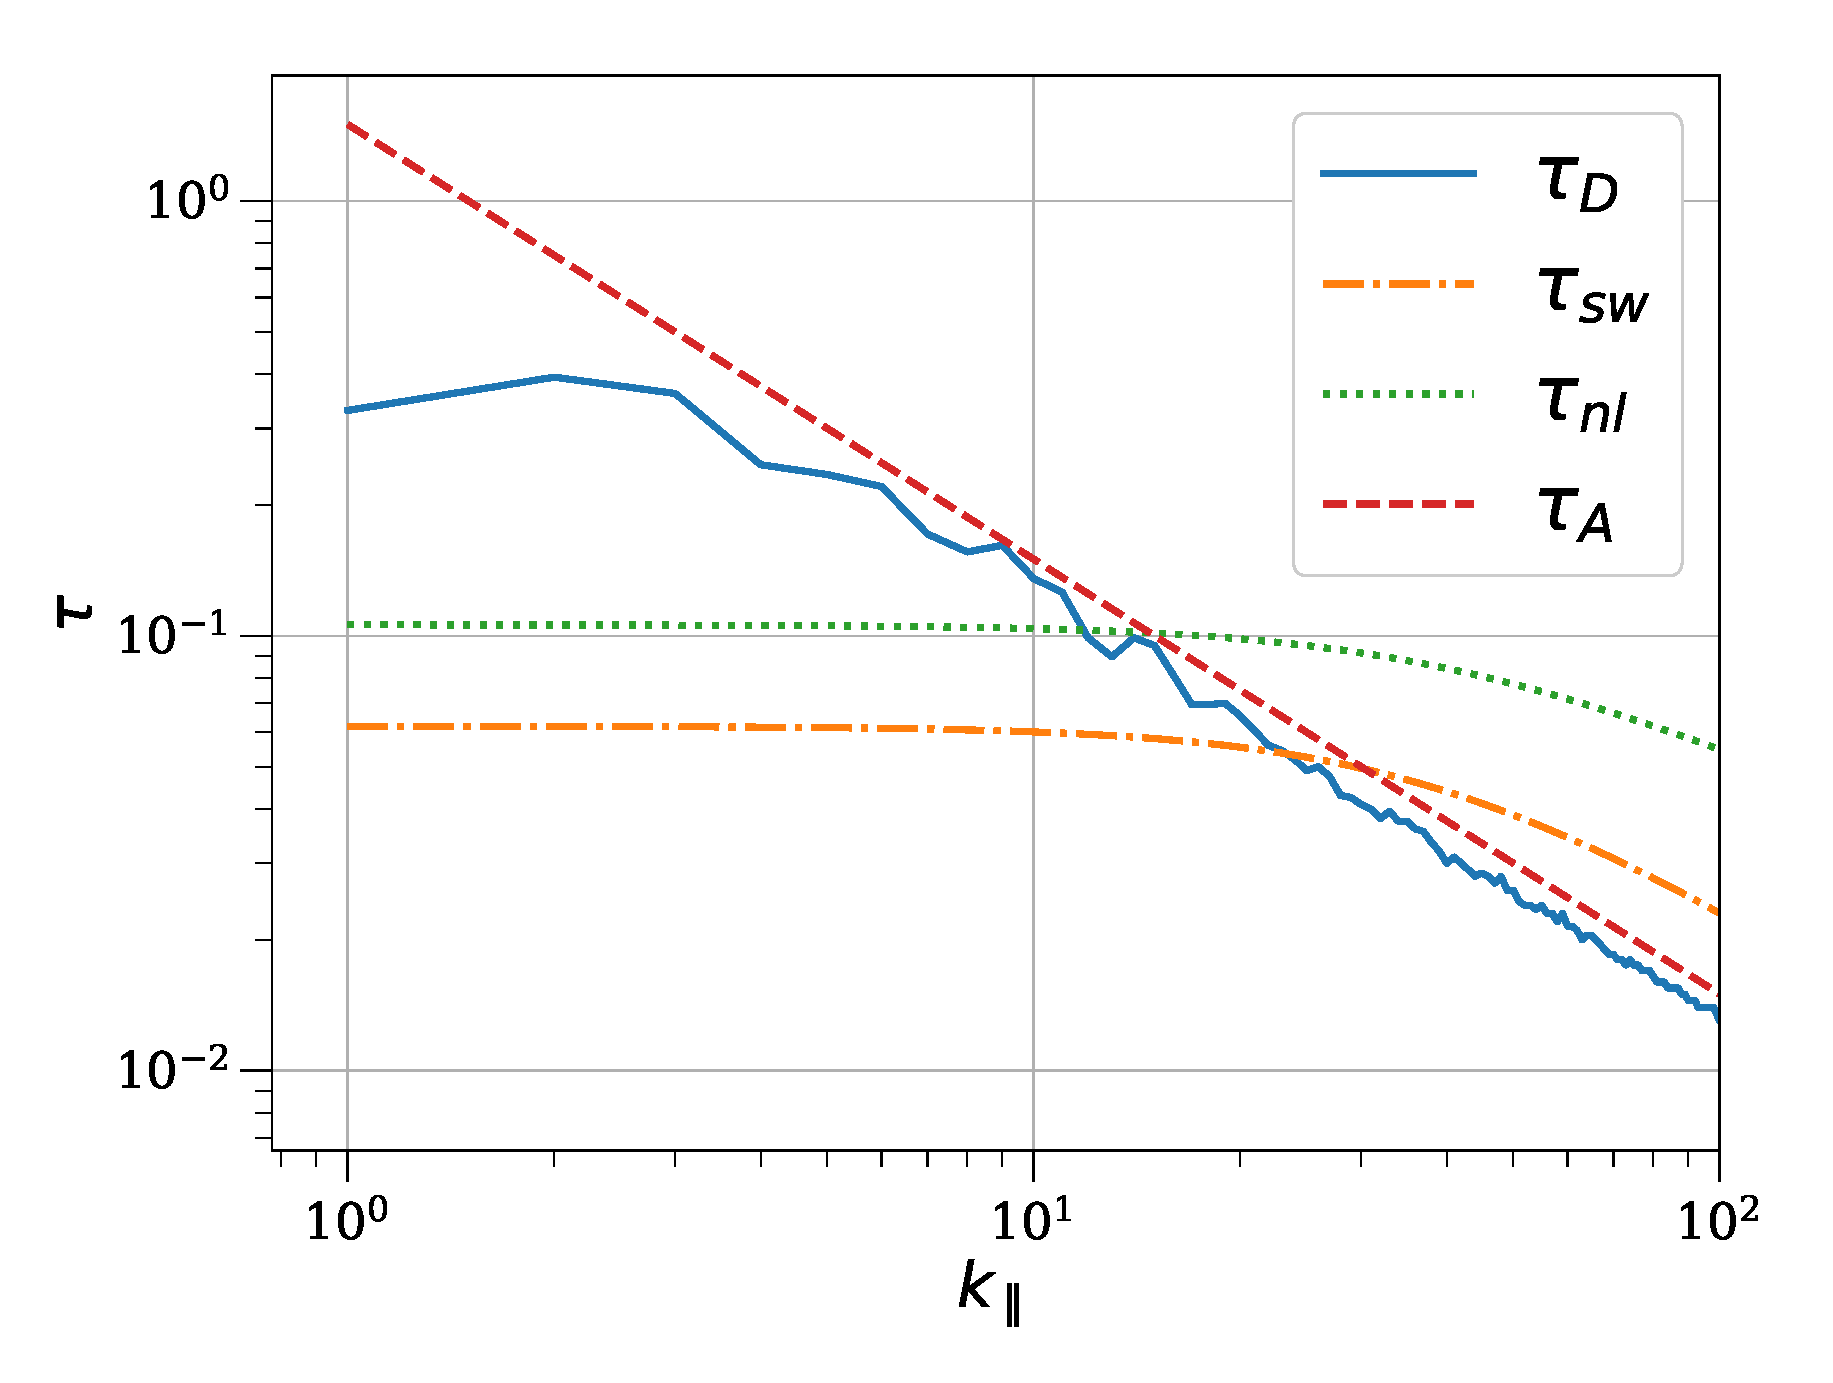
\includegraphics[width=0.95\columnwidth]{CrossHelicity/fig5_B1_Hc09_zpz_kperp_40.eps}}
    \caption{Decorrelation times $\tau_D$ for the runs with $B_0=1$, for $k_\perp=40$ and as a function of $k_\parallel$. The panels correspond to (a) $\sigma_c = 0$, (b) $\sigma_c = 0.3$, and (c) $\sigma_c = 0.9$. The theoretical prediction for the sweeping time $\tau_{sw}$, the non-linear time $\tau_{nl}$, and the Alfv\'en time $\tau_A$ are indicated as references.}
  \label{fig5:tD_vs_Hc}
\end{figure}

A medida que se incrementa el valor de $B_0$, este efecto se vuelve
más evidente. En la \cref{fig3:B1_spectrum_Hc} mostramos el espectro
espacio-temporal para las simulaciones con $B_0=1$. En este caso, la
energía tiende a concentrarse cerca de la relación de dispersión de
las ondas de Alvén para todos los valores de $\sigma_c$; i.e., a
medida que incrementamos el valor de $B_0$, la relevancia del
\sweeping aleatorio decrece, y las ondas de Alfvén se vuelven más
importantes. Para $\sigma_c=0$ observamos ondas propagándose en ambas
direcciones: las fluctuaciones $\vec{z}^+$ se propagan
antiparalelamente al campo guía, y las fluctuaciones $\vec{z}^-$, en
forma paralela a dicho campo. Además, para valores de $k_\parallel$
más grandes que $\approx 20$, la dispersión en la excitación de los
modos se incrementa, y la energíac omienza a poblar el embudo en el
espacio espectral asociado al \sweeping, indicando que el \sweeping
aleatorio juega un rol a escalas verticales suficientemente
pequeñas. En cambio, para $\sigma_c =0.3$ y $0.9$ la energía se
acumula sólo cerca de la relación de dispersión de las ondas, y
recuperamos la contrapropagación de una de las ondas: tanto el campo
$\vec{z}^+$ como el $\vec{z}^-$ se propagan en la misma dirección,
antiparalela al campo guía. Al incrementar aún más $B_0$, este efecto
se reduce (ver el caso con $B_0=8$ en la \cref{fig3:B8_spectrum_Hc}),
resultando en la propagación esperada para cada excitacio, o en muy
poca o ninguna propagación de $\vec{z}^-$ cuando $\sigma_c$ es
suficientemente chico.

¿Cuál es el origen de las fructuaciones $\vec{z}^-$ observadas que se
propagan con el mismo sentido que las fluctuaciones $\vec{z}^+$?
Basado en los resultados de Hollweg \cite{hollweg_1990_wkb}, y en la
\cref{eq:MHD_zpzm}), deben ser causadas por reflexiones en
inhomogeneidades de gran escala del campo magnético medio (notar que
no hay un flujo modio de fondo en nuestras simulaciones, ni
fluctuaciones de densidad).  A pesar de que nuestro campo guía de
fondo $B_0$ es uniforme (i.e., constante tanto en el espacio como en
el tiempo), el campo magnético total incluye una componente fluctuante
lentamente variable (por ejemplo, las fluctuaciones a gran escala,
tales como los modos con $k=1$, que evolucionan en una escala temporal
más lenta que las ondas rápidas y las fluctuaciones de pequeñas
escalas).  Como resultado, el flujo tiene una velocidad de Alvén
efectiva que depende de las coordenadas espaciales. Podemos entonces
escribir para las dos fluctuaciones de Els\"asser la ecuación ideal
linealizada \ref{eq:MHD_zpzm}, con densidad constante y $\vec{U}=0$
(sin flujo medio de fondo), como
\begin{equation}
\partial_t \vec{z}^\pm = \pm \vec{V}_\textrm{A} \cdot \nabla \vec{z}^\pm 
    \mp \vec{z}^\mp \cdot \frac{\nabla \vec{B}'}{\sqrt{4\pi \rho}} ,
\end{equation}
donde $\vec{V}_\textrm{A}$ puede ahora ser incluido en las
fluctuaciones de gran escala del campo magnético, y $\vec{B}'$, como
antes, es el campo magnético total en unidades gaussianas. Si la
helicidad cruzada normalizada es cercana a $1$, es decir, si
$|\vec{z}^+| \gg |\vec{z}^-|$, tenemos que para $\vec{z}^+$
\begin{equation}
\partial_t \vec{z}^+  \approx \vec{V}_\textrm{A} \cdot \nabla \vec{z}^+ ,
\end{equation}
y utilizando $\vec{z}^\pm = \vec{z}_0^\pm e^{i(\vec{k}\cdot
  \vec{x}+\omega^\pm t)}$ recuperamos la relación de dispersión usual
para ondas propagándose antiparalelamente al campo medio $\omega^+ =
+\vec{V}_\textrm{A} \cdot \vec{k}$ (donde ahora $\vec{V}_\textrm{A}$
puede fluctuar lentamente en tiempo y espacio). No obstante, para
$\vec{z}^-$ obtenemos
\begin{equation}
\partial_t \vec{z}^- \approx - \vec{V}_\textrm{A} \cdot \nabla \vec{z}^- + \vec{z}^+ 
    \cdot \frac{\nabla \vec{B}'}{\sqrt{4\pi \rho}} .
\label{eq:zmlinear}
\end{equation}
Esta ecaución indica que la propagación de las perturbaciones
$\vec{z}^-$ (que son más pequeñas en amplitud que $\vec{z}^+$) pueden
ser afectadas fuertemente por el campo $\vec{z}^+$ y por las
variaciones espaciales del campo magnético de gran escala.

De la \cref{eq:zmlinear}, también podemos extraer ciertas condiciones
fenomenológicas para que suceda el comportamiento observado en las
\cref{fig3:B0_spectrum_Hc, fig3:B025_spectrum_Hc, fig3:B1_spectrum_Hc,
  fig3:B8_spectrum_Hc} (y, particularmente, para la contrapropagación
de ondas). Utilizando nuevamente $\vec{z}^\pm = \vec{z}_0^\pm
e^{i(\vec{k}\cdot \vec{x}+\omega^\pm t)}$, y asumiendo $\vec{B}' =
\vec{B}_0' + \vec{b}_0'$ donde $\vec{b}_0' =
\vec{\tilde{b}}_0'e^{i\vec{K} \cdot \vec{x}}$ es el campo magnético de
gran escala lentamente variable, con número de onda $K \ll k$, la
\cref{eq:zmlinear} se reduce a
\begin{equation}
\left( \omega^- +\vec{V}_\textrm{A} \cdot \vec{k} \right) 
    \vec{z}_0^- e^{i \omega^- t} = 
    \frac{\left(\vec{K} \cdot \vec{z}_0^+\right) \vec{b}_0'}{\sqrt{4\pi \rho}} 
    e^{i \omega^+ t} .
\end{equation}
Tomando el producto escalar con $\vec{z}_0^-$, definiendo las
densidades energéticas de Els\"asser $e^\pm = |\vec{z}_0^\pm|^2/4$, y
definiendo las fluctuaciones en la velocidad de Alfvén (asociadas a
las fluctuaciones de gran escala del campo magnético) como
$\vec{v}_\textrm{A} = \vec{b}_0'/\sqrt{4\pi \rho}$, obtenemos
\begin{equation}
\left( \omega^- + \vec{V}_\textrm{A} \cdot \vec{k} \right)
    e^{i \omega^- t} = 
    \frac{\left(\vec{K} \cdot \vec{z}_0^+\right)
    \left(\vec{v}_\textrm{A} \cdot \vec{z}_0^-\right)}
    {4e^-} 
    e^{i \omega^+ t} .
\end{equation}
Esta ecuación admite como soluciones
\begin{eqnarray}
    \omega^- &=& \omega^+ =
    + \vec{V}_\textrm{A} \cdot \vec{k}, 
    \label{eq:cond1} \\
    2 \vec{V}_\textrm{A} \cdot \vec{k} &=& 
    \left(\vec{K} \cdot \vec{z}_0^+\right)
    \left(\vec{v}_\textrm{A} \cdot \vec{z}_0^-\right) /
    (4e^-), \label{eq:cond2}
\end{eqnarray}
que corresponde a ambas ondas viajando en la misma dirección mientras
la segunda condición, dada por la \cref{eq:cond2}, pueda ser
cumplida. A partir de análisis dimensional, esta condición requiere
que
\begin{equation}
    2 \frac{V_\textrm{A}}{v_\textrm{A}} \frac{k}{K}
    \sim \sqrt{\frac{e^+}{e^-}},
\end{equation}
que (como $V_\textrm{A}\gtrsim v_\textrm{A}$ y $k\gg K$) no puede ser
satisfecha cuando $\sigma_c \approx 0$ (como se observa en las
\cref{fig3:B0_spectrum_Hc, fig3:B025_spectrum_Hc, fig3:B1_spectrum_Hc,
  fig3:B8_spectrum_Hc}, o cuando el campo guía se vuelve demasiado
fuerte para un valor dijo de $\sigma_c$ (como también fue observado en
los espectros espacio-temporales). Así, este último argumento
cualitativo indica (en acuerdo con las simulaciones) que las
fluctuaciones $\vec{z}^-$ pueden propagarse con la misma velocidad de
fase y dirección que las fluctuaciones $\vec{z}^+$, siempre que
$\sigma_c \neq 0$ y $B_0$ no sea demasiado fuerte para un valor fijado
de la helicidad cruzada normalizada.

En otras palabras, si $|\vec{z}^+|$ a grandes escalas en comparable
con $|\vec{V}_\textrm{A}|$ y $\sigma_c \approx 1$, podemos ver que las
fluctuaciones $\vec{z}^-$ se prapagan en la misma dirección que las
fluctuaciones $\vec{z}^+$ como resultado de reflexiones en
inhomogeneidades del campo magnético de gran escala.  Un
comportamiento similar puede resultar, por ejemplo, a partir de
fluctuaciones en la densidad de masa cuando el fluido es compresible,
como es en caso de algunas regiones del viendo solar y en el medio
interplanetario \cite{zhou_1989_nonWKBevolution}, y este argmumento no
imposibilita a otros efectos, tales como interacciones fuertes no
lineales, de resultar en reflexiones y contrapropagaciones de las
excitaciones. Es más, cuando la intensidad del campo magnético de
fondo se aumenta aún más, los argumentos utilizados dejan de ser
válidos, y la relevancia de las reflexiones se reduce. Esto es
compatible con el comportamiento observado en la
\cref{fig3:B8_spectrum_Hc} para la simulación con $B_0=8$, la cual
muestra una potencia similar en ambos tipos de fluctuaciones cuando
$\sigma_c=0$, menos potencia en las fluctuaciones $\vec{z}^-$ cuando
$\sigma_c=0.3$ (y propagándose en dirección opuesta al campo
$\vec{z}^+$), y una cantidad no apreciable de potencia para las
fluctuaciones $\vec{z}^-$ (en comparación con $\vec{z}^+$) en el caso
con $\sigma_c=0.9$.

\subsection{Tiempos de descorrelación}

A partir de las discusiones en la sección
\ref{sec_Wfspectrum_and_Gamma}, otra forma de identificar la escala
temporal dominante para modos individuales es estudiar el tiempo de
descorrelación $\tau_D$, i.e., el tiempo que le toma a cada modo de
Fourier con vector de onda $\vec{k}$ estar descorrelacionado de su
historia previa, ya sea por interacciones no lineales con
\textit{eddies} (si $\tau_D \sim \tau_{nl}$), por {\color{red}
  cross-over of waves} (si $\tau_D \sim \tau_A$), o por \sweeping del
flujo de gran escala (cuando $\tau_D \sim \tau_{sw}$). Nuevamente,
como $\tau_D$ depende del vector de onda $\vec{k}$, en lo que sigue
mostraremos los resultados para valores fijos de $k_\parallel$ o
$k_\perp$, y en función del número de onda restante. En todos los
casos, el tiempo de descorrelación $\tau_D$ es obtenido a partir de
datos numéricos computando la función de correlación
$\Gamma(k_{\perp},k_{\parallel},\tau)$, y buscando los valores del
{\color{red} time lag} $\tau$ para los cuales la función de
correlación decae a un valor $1/e$ de su valor para $\tau=0$, es
decir, el tiempo característico para el decaimiento de la función de
correlación \cite{lugones_2016_spatiotemporal}.

La \cref{fig5:z+_vs_z-} muestra los diferentes tiempos de
descorrelación para un valor fijo de $k_{\parallel}=10$ y en función
de $k_{\perp}$, para la simulación con $B_0=1$ y
$\sigma_c=0.3$. También se indican como referencia las predicciones
teóricas para los diferentes tiempos de descorrelación. Como el tiempo
de Alfvén es independiente de $k_{\perp}$, se ve con un valor
constante en dicha figura.El tiempo de descorrelación $\tau_D$
obtenido de los datos numéricos se encuentra muy cercano al tiempo de
Alfvén para valores pequeños de $k_{\perp}$ (hasta $k_\perp \approx
10$), pero luego se desvía y se acerca al tiempo de \sweeping para
valores grandes de $k_{\perp}$ (i.e, para pequeñas escalas
perpendiculares). Esto se ve más claro para las fluctuaciones
$\vec{z}^-$ que para las fluctuaciones $\vec{z}^+$, para las cuales el
tiempo de descorrelación $\tau_D$ para $k_\perp > 10$ se encuentra
entre los escaleos de $\tau_{sw}$ y de $\tau_{nl}$.

La \cref{fig5:tD_vs_B0} muestra el tiempo de descorrelación $\tau_D$
del campo $\vec{z}^+$ para los casos con $\sigma_c = 0.3$, con campos
guía de $B_0=0.25$, $1$, $4$, y $8$, y para el caso $k_\parallel = 15$
en función de $k_\perp$.  Nuevamente, para balores bajos de $B_0$,
$\tau_D$ está mayoritariamente dominado por el \sweeping, o bien para
todos los valores de $k_\perp$ para el caso con $B_0=0.25$, o bien por
debajo de $k_\perp \approx 20$ para $B_0=1$. Sin embargo, para valores
más altos de $B_0$ (o para pequeños valores de $k_\perp$ cuando
$B_0=1$) los efectos Alfvénicos se vuelven dominantes, con $\tau_D$
tomando valores cercanos al $\tau_{A}$. En general, la escala temporal
más rápida a todos los valores parece ser la escala dominante. Estos
resultados son consistentes con los obtenidos previamente en
\cite{lugones_2016_spatiotemporal} para el caso de turbulencia MHD
fuerte incompresible con helicidad cruzada nula, aunque la presencia
de helicidad cruzada baja en el flujo parece favorecer la transición
hacia un flujo más dominado por las ondas de Alfvén, como también
vimos en los espectros espacio-temporales en la sección
\ref{sec:wk}. Esto puede ser asociado con el hecho de que bajo ciertas
condiciones, el tiempo no lineal de la fluctuación de Els\"asser
dominantes se vuelve muy grande, y la escala temporal de
descorrelación es entonces determinada por las llamadas ``especies
minoritarias'', como se reportó anteriormente en los cálculos de
clausura de Grappin \textit{et al.} \cite{grappin_1983_dependence}.

Este comportamiento puede ser también visto cuando la variable fijada
es $k_\perp$, y $\tau_D$ es estudiada en función de $k_\parallel$ (ver
la \cref{fig5:tD_vs_B0_2}). Para las simulaciones con $\sigma_c=0.3$ y
con $B_0$ incrementándose, vemos que $\tau_D$ varía con $k_\parallel$
como $\tau_{sw}$ cuando $B_0$ es pequeño o moderado y cuando
$k_\parallel$ es pequeño, y varía como $\tau_A$ cuando $B_0$ o
$k_\parallel$ son suficientemente grandes. En otras palabras, los
modos con vectores de onda suficientemente alineados con el campo guía
son dominados por el tiempo de Alfvén. Y nuevamente, la escala
temporal más rápida en esta figura es la que domina la dinámica.

No obstante, como mencionamos anteriormente, este panorama cambia
cuando $\sigma_c$ es suficientemente grande. Esto puede verse en la
figura \cref{fig5:tD_vs_Hc}, donde se grafica el tiempo de
descorrelación $\tau_D$ para las simulaciones con $B_0=1$, para
$k_\perp=40$ fijo, y en función de $k_\parallel$ para $\sigma_c = 0$,
$0.3$ y $0.9$. Mientras que para valores pequeños de $\sigma_c$ se
observa el mismo comportamiento que lo anterior, para valores grandes
de $\sigma_c$ el tiempo de Alfvén se vuelve dominante, aun cuando es
más lento que las otras escalas temporales, como se ve en las
simulaciones con $\sigma_c=0.9$ y valores pequeños de $k_\parallel$.

Así, mientras que para pequeños valores de $\sigma_c$ el análisis del
tiempo de descorrelación confirma la tendencia observada en nuestro
estudio previo \cite{lugones_2016_spatiotemporal}, en el que el tiempo
de \sweeping domina la descorrelación excepto para los casos con
valores medios y largos de $B_0$, donde el tiempo Alfvénico es
dominante para valores pequeños de $k_{\perp}$ o valores grandes de
$k_{\parallel}$ (ver también los estudios de turbulencia MHD débil, o
de la transición de turbulencia MHD débil a fuerte en las referencias
\cite{meyrand_weak_2015, lugones_2016_spatiotemporal,
  meyrand_direct_2016}), incrementando la helicidad cruzada del flujo
tiene consecuencias muy interesantes.  La aparición del tiempo de
Alfvén como el dominante se vuelve más claro para valores altos de
$\sigma_c$, aún cuando no es la escala temporal más rápida, y es
consistente con la imagen en la que la mayoría de las fluctuaciones
tienen una única dirección de propagación.  Sin embargo, como se
evidencia en el análisis espacio-temporal del espectro energético en
cada uno de los campos de Els\"asser en función de $\vec{k}$ y
$\omega$, las inhomogeneidades de las escalas grandes del campo
magnético pueden inducir reflexiones, y pueden {\color{red} prender}
interacciones no lineales dominadas por el {\color{red} Alfv\'en
  cross-over time} entre las ondas para modos con vectores de onda
suficientemente alineados con el campo guía, o por el \sweeping o el
tiempo no lineal para otros modos.

%%%%%%%%%%%%%%%%%%%%%%%%%%%%%%%%%%%%%%%%5
\section{Conclusiones}\label{sec_Conclusions}

Analizamos el comportamiento espacio-temporal de las fluctuaciones MHD
considerando sus polarizaciones en términos de las variables de
Els\"asser, utilizando simulaciones numéricas directas
tridimensionales de turbulencia MHD incompresible. Consideramos casos
con valores bajos, intermedios y altos de campo magnético medio de
fondo, y con helicidad cruzada nula, pequeña y alta. Las funciones de
correlación como función de los vectores de onda (descompuestos en las
direcciones perpendicular y paralela del campo magnético medio) y del
tiempo de retraso fue directamente computada para todas las diferentes
simulaciones consideradas, así como también los espectros
espacio-temporales. A partir de las funciones de correlación,
computamos el tiempo de descorrelación para cada modo de Fourier, y lo
comparamos con las diferentes predicciones teóricas para las escalas
temporales relevantes en el sistema: el tiempo no lineal local, el
\sweeping aleatorio y el tiempo Alfvénico. Se observó que los tiempos
de descorrelación son dominados por los efectos de \sweeping para
valores bajos del campo magnético medio y de la helicidad cruzada,
mientras que para valores grandes del campo magnético medio o de
helicidad cruzada, los tiempos de descorrelación están controlados por
los efectos Alfvénicos aún cuando el tiempo de Alfvén no sea el más
rápido, una nueva característica cuando lo comparamos con estudios
previos del comportamiento espacio-temporal de turbulencia MHD fuerte
con helicidad cruzada nula. En principio, este comportamiento puede
ser interpretado como una transición hacia un refimen con
no-linealidades más débiles a medida que se incrementa la helicidad
cruzada, como suele ser discutido teóricamente y como aparentemente
indican nuestras simulaciones numéricas.

Sin embargo, debe notarse que los espectros espacio-temporales indican
que aún en este regimen, las interacciones no lineales son
relevantes. El otro resultado principal obtenido de nuestro análisis
es el haber encontrado un regimen en el que se generan fluctuaciones
$\vec{z}^-$ y $\vec{z}^+$, polarizaciones opuestas, y se propagan en
la misma dirección debido a la reflexión de ondas, causada por
inhomogeneidades del campo magnético de gran escala. Esto es más
evidente en los espectros espacio-temporales de los campos de
Els\"asser para valores intermedios del campo magnético de fondo (es
decir, cuando la componente uniforme y constante del campo magnético
de gran escala no es demasiado fuerte). Un análisis fenomenológico
basado en ideas previas en Zhou and Matthaeus \cite{zhou1990remarks}
confirma las conclusiones de \cite{hollweg_1990_wkb}, que indican que
las fluctuaciones Alfvénicas con polarizaciones opuestas pueden
efectivamente propagarse en la misma dirección y aún con la misma
velocidad.  Si el campo magnético de fondo se vuelve demasiado fuerte
(o si la helicidad cruzada se acerca a cero), este efecto no se
observa más. Así, el análisis espacio-temporal de los flujos
turbulentos provee evidencia directa de un fenómeno predicho
anteriormente con la teoría WKB, y puede jugar un rol relevando
modificando la propagación de ondas y las interacciones no lineales en
el medio interplanetario.

Los resultados analizados en este trabajo muestran en detalle que, al
menos en el regimen de turbulencia fuerte, la representación de ondas
no es suficientemente completa para describir el sistema de MHD
incompresible. En este sistema aparece una amplia banda de
fluctuaciones provenientes de efectos locales y no locales
(\sweeping), que generan dispersión y efectos no lineales. Es
importante recordar, por supuesto, que gran parte del presente estudio
se ha concentrado en el estudio del tiempo de decorrelación euleriano,
descompuesto en un tiempo de decorrelación dependiente de la escala de
los modos de Fourier individuales. Esta descorrelación generalmente se
interpreta como una competencia entre la descorrelación por \sweeping
por fluctuaciones a gran escala y la decorrelación que se origina en
la propagación de ondas. Sin embargo, ninguno de estos efectos es en
principio responsable de la transferencia espectral que da lugar a la
cascada de turbulencias. De hecho, el efecto principal de la
propagación de Alfvén, desde la perspectiva de la cascada energética
en turbulenta fuerte, no es causar transferencia espectral sino
suprimirla \cite{shebalin_1983_anisotropy}. La comprensión de la
cascada en sí misma requiere examinar la fuerza de las no
linealidades. En este caso, el tiempo característico apropiado se
convierte en el tiempo no lineal, cuyo aislamiento requiere el
análisis de escalas de tiempo en el marco lagrangiano
\cite{kraichnan_1964_kolmogorov} (teera en cuenta que sólo en algunos
casos particulares en nuestro análisis, el tiempo no lineal se
identificó positivamente como un candidato para el tiempo de
descorrelación). Sin embargo, hemos demostrado que fenómenos
físicamente relevantes como la reflexión y la `` propagación anómala
'' de fluctuaciones reflejadas pueden producir efectos observables en
la energía del flujo, y estos fenómenos se han reconocido en una
variedad de configuraciones de los diferentes parámetros de control
del sistema, con posibles aplicaciones.

Por ejemplo, efectos interesantes asociados con la reflexión se suman
a la complejidad de la dinámica, incluso en el caso más simple de MHD
incompresible considerado aquí. Esto tiene implicaciones importantes
para aplicaciones como el calentamiento coronal, la aceleración del
viento solar y la energización de partículas en el espacio
interplanetario \cite{velli_1993_propagation, matthaeus_1999_coronal}.
Como otro ejemplo, las fluctuaciones observadas en el viento solar,
que tienden a alinear o antialinear el campo magnético y el campo de
velocidad (es decir, con diferentes polarizaciones Alfvénicas), no
siempre se pueden interpretar trivialmente como viajando
``downstream'' o ``upstream'' respecto del campo magnético medio.
Extensiones de este estudio a MHD compresible
\cite{andres_2017_interplay}, considerando la dependencia con la
helicidad cruzada en el flujo y su interacción con los efectos
compresibles, así como un estudio que considera otras helicidades como
la helicidad cinética $H_v$, la helicidad magnética $H_b$ y la
helicidad híbrida para Hall-MHD, sería un seguimiento interesante del
presente estudio y un primer paso hacia una comprensión más profunda
del papel de los efectos no lineales en la propagación de ondas en la
turbulencia en plasma.

